\section{Measurement of Dijet Mass Spectrum}

In this section we explain how we measure the 
dijet mass spectrum in data, compare it with
the Monte Carlo predictions for QCD, and fit it
to a simple parameterization to test the smoothness 
of the data.

\subsection{Data Sample}

Our collision dataset was 
\begin{verbatim}

  ===Calo, PF Jet===
  
  (136033-141949)  /JetMETTau/Run2010A-Apr21ReReco-v1/AOD
  (141950-145761)  /JetMET/Run2010A-Apr21ReReco-v1/AOD
  (145762-149442)  /Jet/Run2010B-Apr21ReReco-v1/AOD
  (160404-163869)  /Jet/Run2011A-May10ReReco-v1/AOD
  (165088-165970)  /Jet/Run2011A-PromptReco-v4/AOD

  ===Wide Jet===

  (160404-163869)  /HT/Run2011A-May10ReReco-v1/AOD
  (165088-167784)  /HT/Run2011A-PromptReco-v4/AOD

\end{verbatim}
The reconstruction software (CMSSW\_4\_2\_1\_patch1) is used for /JetMETTau/Run2010A-Apr21ReReco-v1/AOD, /JetMET/Run2010A-Apr21ReReco-v1/AOD and /Jet/Run2010B-Apr21ReReco-v1/AOD.
The reconstruction software (CMSSW\_4\_2\_3) is used for /Jet/Run2011A-May10ReReco-v1/AOD and /HT/Run2011A-May10ReReco-v1/AOD.
The reconstruction software (CMSSW\_4\_2\_3\_patch1), (CMSSW\_4\_2\_3\_patch2), (CMSSW\_4\_2\_3\_patch3), (CMSSW\_4\_2\_3\_patch5) are used for /Jet/Run2011A-PromptReco-v4/AOD and /HT/Run2011A-PromptReco-v4/AOD.
We run over this dataset at the Fermilab LPC and CERN.

The good run and luminosity section (LS) selection is based on the official CMS JSON files:
\begin{verbatim}

(136033-149442)
/afs/cern.ch/cms/CAF/CMSCOMM/COMM_DQM/certification/Collisions10
/7TeV/Reprocessing/Cert_136033-149442_7TeV_Apr21ReReco_Collisions10_JSON.txt
(160404-163869)
/afs/cern.ch/cms/CAF/CMSCOMM/COMM_DQM/certification/Collisions11
/7TeV/Reprocessing/Cert_160404-163869_7TeV_May10ReReco_Collisions11_JSON.txt
(163870-167784)
/afs/cern.ch/cms/CAF/CMSCOMM/COMM_DQM/certification/Collisions11
/7TeV/Prompt/Cert_160404-167784_7TeV_PromptReco_Collisions11_JSON.txt

\end{verbatim}
The integrated luminosity of the selected sample for
WideJets, all 2011 data from the unprescaled HT trigger~\cite{CMS_AN_2011/242}, 
is estimated to be $1.01\,fb^{-1}$ with a systematic uncertainty of 6\%. The integrated luminosity of the
CaloJet and PFjet samples, both 2010 and 2011 data from the unprescaled single jet trigger, is estimated to be $1.01\,fb^{-1}$.

We require that each event has a good primary vertex with $z$ value
within 24 cms of the center of the detector and a number of degrees of
freedom of at least 4. Finally, we only keep jets with corrected $p_T>30$ GeV.
This preselection job writes out ROOT trees from the skimmed AOD dataset
on cmslpc.fnal.gov.

\subsection{MC Samples}

\subsubsection{QCD}
For the comparison between data and simulation, we use the QCD Pythia
MC where the phase space is divided into 20 exclusive bins, based on
the transverse momentum of the hard scattered parton ($\hat{p}_T$).
The MC samples used are:
\begin{verbatim}
/QCD_Pt-XXtoYY_TuneZ2_7TeV_pythia6/Summer11-PU_S3_START42_V11-v2/AODSIM
/QCD_Pt-XX_TuneZ2_7TeV_pythia6/Summer11-PU_S3_START42_V11-v2/AODSIM
\end{verbatim}
where XX and YY stand for the $\hat{p}_T$ boundaries. For the final
comparison with the data, the MC samples are weighted according to the
cross-section and the number of events that were used.

\subsubsection{Resonances}
For resonance shapes we use the PYTHIA MC for excited quarks (Qstar)
and Randall Sundrum Gravitons (RSGraviton) as discussed in the next
section.  The samples used were
\begin{verbatim}
/ResonanceToJJ_M-XX_TuneD6T_7TeV_pythia6/Summer11-PU_S4_START42_V11-v1/AODSIM
\end{verbatim}
where RESONANCE is either "Qstar" or "RSGraviton", XX is 500, 700, 1200, 2000 or
3500 for those masses in GeV.

\subsection{Software}
The analysis was done using the 
$CMSSW\_4\_2\_5$ release and the software is available in the CMS CVS through the following
tags:
\begin{verbatim}
V00-02         Analysis/Statistics                              
V00-04-01      KKousour/QCDAnalysis 
\end{verbatim}

\subsection{Jet Reconstruction}


Jets are reconstructed using the anti-$k_T$ algorithm~\cite{1126-6708-2008-04-063} with cone size 
$R=\sqrt{(\Delta\eta)^2 + (\Delta\phi)^2}=0.7$.  This analysis uses three types of jets:
calorimeter jets, particle flow jets and wide jets. Calorimeter jets use calorimeter energy deposits as
input to the jet reconstruction algorithm.  Particle flow~\cite{PFT-09-001-PAS} attempts to reconstruct all stable particles in an 
event by combining information from all subdetectors. Particle flow categorizes all particles 
into the following five types: muons, electrons, photons, charged and neutral hadrons. Particle
flow jets use reconstructed particles as the set of inputs to the jet reconstruction algorithm.
The reconstructed jet energy, $E$, is defined as the scalar sum of the energies of the inputs 
to the jet and the jet momentum, $\vec{p}$, is the corresponding vector sum of the momenta of
the inputs. The jet transverse momentum, $p_T$, is the component
of $\vec{p}$ in the transverse plane.
The $E$ and $\vec{p}$ of a reconstructed jet are then corrected for the
response of the reconstructed jet to a generated jet, using Monte Carlo 
simulation~\cite{PAS_JME_10-011}.  
Generated jets come
from applying the same jet algorithm to the Lorentz vectors of stable generated particles before detector simulation.
The corrections are chosen so that, on average, the $p_T$ of a
corrected jet is equal to the $p_T$ of the corresponding generated jet. This 
includes a correction for pile-up of multiple pp interactions in the event.
We combine particle flow jets with $p_T>10$ GeV within $\Delta R<1.1$ to obtain wide jets as 
shown in Fig.~\ref{Wide_definition}.  The wide jet algorithm we use is described in more 
detail elsewhere~\cite{CMS_AN_2011/242}.
This analysis uses particle flow wide jets for the search and particle flow jets and calojets as a check,
and all figures show wide jets unless otherwise noted.


\begin{figure}[!ht]
  \begin{center}
    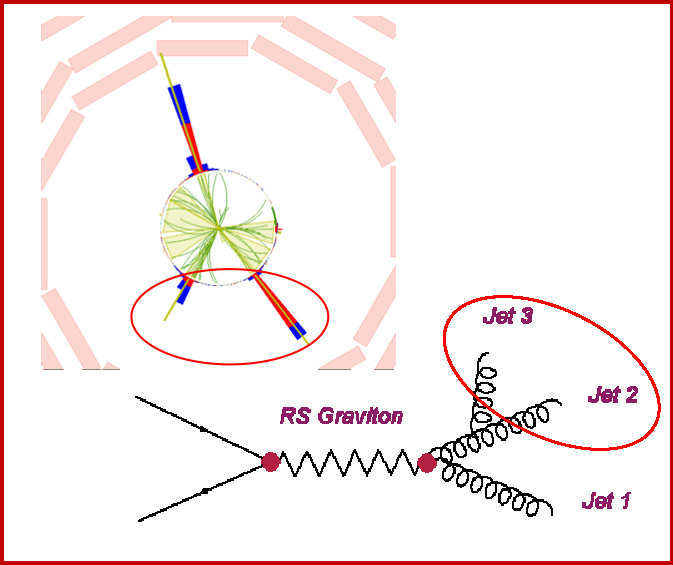
\includegraphics[width=0.45\textwidth]{Figures/fat_definition.pdf}
    \caption{ Wide jets are made by combining PF jets }
    \label{Wide_definition}
  \end{center}
\end{figure}



The corrections used for the MC were the CMS standard relative
(L2) and absolute(L3) jet corrections for $\eta$ and $p_T$ variation
of the jet response using tag "Summer11". 
The corrections used for the data, as recommended by JetMET, were the (L2) and absolute(L3) jet 
corrections for $\eta$ and $p_T$ variation from "special 3\_11\_1\_hclpatch1 MC" and the L1FastJet(PF,wide), L1Offset(Calo)
correction for pile-up.

%A residual data-driven relative (L2) correction derived from dijet
%balance, using the same sample, is applied to the data to correct for
%differences between data and MC: the method and correction is
%described for a smaller sample~\cite{PAS_JME_10-003, CMS_AN_2010/139}.

The dijet system is composed of the two jets with the highest $p_T$ in
an event (leading jets), and the dijet mass is given by $m=\sqrt{(E_1
+ E_2)^2 - (\vec{p}_1 + \vec{p}_2)^2}$.

We run our configuration file on AOD dataset to produce a single
``Processed'' ROOT tree. In this step we select the Anti-KT 0.7 jets
and apply the jet corrections.  We select events that have passed 
high level trigger paths listed in the table. ~\ref{table:HLTdescriptions_Jet} and perform a
jet $p_T$ preselection of $p_T>40$ GeV (corrected) for Calo and PF jets.  From the
processed trees we perform the final analysis.

\begin{table}[th]
  \centering
  \normalsize
  \begin{tabular}{|c|c||c|c|}
    \hline
    Trigger Path     & L1 seeds          & Trigger Path    & L1 seeds        \\
    \hline 
    \hline
    L1\_SingleJet16  &  none             & HLT\_Jet80\_v1  & L1\_SingleJet52 \\
    \hline
    L1\_SingleJet36  &  none             & HLT\_Jet80\_v2  & L1\_SingleJet52 \\
    \hline
    L1\_SingleJet52  &  none             & HLT\_Jet80\_v3  & L1\_SingleJet52 \\
    \hline
    L1\_SingleJet68  &  none             & HLT\_Jet80\_v4  & L1\_SingleJet52 \\
    \hline
    L1\_SingleJet92  &  none             & HLT\_Jet80\_v5  & L1\_SingleJet52 \\
    \hline
    L1\_SingleJet6U  &  none             & HLT\_Jet80\_v6  & L1\_SingleJet52 \\
    \hline
    L1\_SingleJet20U &  none             & HLT\_Jet110\_v1  & L1\_SingleJet68 \\
    \hline
    L1\_SingleJet30U &  none             & HLT\_Jet110\_v2  & L1\_SingleJet68 \\
    \hline
    L1\_SingleJet40U &  none             & HLT\_Jet110\_v3  & L1\_SingleJet68 \\
    \hline
    L1\_SingleJet60U &  none             & HLT\_Jet110\_v4 & L1\_SingleJet68 \\
    \hline
    HLT\_Jet15U      &  L1\_SingleJet6U  & HLT\_Jet110\_v5 & L1\_SingleJet68 \\
    \hline
    HLT\_Jet15U\_v3  &  L1\_SingleJet6U  & HLT\_Jet110\_v6 & L1\_SingleJet68 \\
    \hline
    HLT\_Jet30U      &  L1\_SingleJet20U & HLT\_Jet150\_v1 & L1\_SingleJet92 \\
    \hline
    HLT\_Jet30U\_v3  &  L1\_SingleJet20U & HLT\_Jet150\_v2 & L1\_SingleJet92 \\
    \hline
    HLT\_Jet50U      &  L1\_SingleJet30U & HLT\_Jet150\_v3 & L1\_SingleJet92 \\
    \hline
    HLT\_Jet15U      &  L1\_SingleJet6U  & HLT\_Jet150\_v4 & L1\_SingleJet92 \\
    \hline
    HLT\_Jet15U\_v3  &  L1\_SingleJet6U  & HLT\_Jet150\_v5 & L1\_SingleJet92 \\
    \hline
    HLT\_Jet30U      &  L1\_SingleJet20U & HLT\_Jet150\_v6 & L1\_SingleJet92 \\
    \hline
    HLT\_Jet30U\_v3  &  L1\_SingleJet20U & HLT\_Jet190\_v1 & L1\_SingleJet92 \\
    \hline
    HLT\_Jet50U      &  L1\_SingleJet30U & HLT\_Jet190\_v2 & L1\_SingleJet92 \\
    \hline
    HLT\_Jet50U\_v3  &  L1\_SingleJet30U & HLT\_Jet190\_v3 & L1\_SingleJet92 \\
    \hline
    HLT\_Jet70U      &  L1\_SingleJet30U & HLT\_Jet190\_v4 & L1\_SingleJet92 \\
    \hline
    HLT\_Jet70U\_v2  &  L1\_SingleJet40U & HLT\_Jet190\_v5 & L1\_SingleJet92 \\
    \hline
    HLT\_Jet70U\_v3  &  L1\_SingleJet40U & HLT\_Jet190\_v6 & L1\_SingleJet92 \\
    \hline
    HLT\_Jet100U     &  L1\_SingleJet30U & HLT\_Jet240\_v1 & L1\_SingleJet92 \\
    \hline
    HLT\_Jet100U\_v2 &  L1\_SingleJet60U & HLT\_Jet240\_v2 & L1\_SingleJet92 \\
    \hline
    HLT\_Jet100U\_v3 &  L1\_SingleJet60U & HLT\_Jet240\_v3 & L1\_SingleJet92 \\
    \hline
    HLT\_Jet140U\_v1 &  L1\_SingleJet60U & HLT\_Jet240\_v4 & L1\_SingleJet92 \\
    \hline
    HLT\_Jet140U\_v3 &  L1\_SingleJet60U & HLT\_Jet240\_v5 & L1\_SingleJet92 \\
    \hline
    HLT\_Jet180U\_v3 &  L1\_SingleJet60U & HLT\_Jet240\_v6 & L1\_SingleJet92 \\
    \hline
    HLT\_Jet30\_v1   &  L1\_SingleJet16  & HLT\_Jet300\_v1 & L1\_SingleJet92 \\
    \hline
    HLT\_Jet30\_v2   &  L1\_SingleJet16  & HLT\_Jet300\_v2 & L1\_SingleJet92 \\
    \hline
    HLT\_Jet30\_v3   &  L1\_SingleJet16  & HLT\_Jet300\_v3 & L1\_SingleJet92 \\
    \hline
    HLT\_Jet30\_v4   &  L1\_SingleJet16  & HLT\_Jet300\_v4 & L1\_SingleJet92 \\
    \hline
    HLT\_Jet30\_v5   &  L1\_SingleJet16  & HLT\_Jet300\_v5 & L1\_SingleJet92 \\
    \hline
    HLT\_Jet30\_v6   &  L1\_SingleJet16  & HLT\_Jet370\_v1 & L1\_SingleJet92 \\
    \hline
    HLT\_Jet60\_v1   &  L1\_SingleJet36  & HLT\_Jet370\_v2 & L1\_SingleJet92 \\
    \hline
    HLT\_Jet60\_v2   &  L1\_SingleJet36  & HLT\_Jet370\_v3 & L1\_SingleJet92 \\
    \hline
    HLT\_Jet60\_v3   &  L1\_SingleJet36  & HLT\_Jet370\_v4 & L1\_SingleJet92 \\
    \hline
    HLT\_Jet60\_v4   &  L1\_SingleJet36  & HLT\_Jet370\_v5 & L1\_SingleJet92 \\
    \hline
    HLT\_Jet60\_v5   &  L1\_SingleJet36  & HLT\_Jet370\_v6 & L1\_SingleJet92 \\
    \hline
    HLT\_Jet60\_v6   &  L1\_SingleJet36  & HLT\_Jet800\_v1 & L1\_SingleJet92 \\
    \hline

  \end{tabular}
  \caption{L1 and High Level Jet Triggers}
  \label{table:HLTdescriptions_Jet}
\end{table}

\begin{table}[th]
  \centering
  \normalsize
  \begin{tabular}{|c|c||c|c|}
    \hline
    Trigger Path     & L1 seeds          & Trigger Path    & L1 seeds        \\
    \hline 
    \hline
    L1\_HTT50        & none              & HLT\_HT300\_v2  & L1\_HTT100      \\
    \hline
    L1\_HTT75        & none              & HLT\_HT300\_v3  & L1\_HTT100      \\
    \hline
    L1\_HTT100       & none              & HLT\_HT300\_v4  & L1\_HTT100      \\
    \hline
    HLT\_HT100U      & L1\_HTT50         & HLT\_HT300\_v5  & L1\_HTT100      \\
    \hline
    HLT\_HT100U\_v3  & L1\_HTT50         & HLT\_HT300\_v6  & L1\_HTT100      \\
    \hline
    HLT\_HT120U      & L1\_HTT50         & HLT\_HT300\_v7  & L1\_HTT100      \\
    \hline
    HLT\_HT130U\_v3  & L1\_HTT50         & HLT\_HT300\_v8  & L1\_HTT100      \\
    \hline
    HLT\_HT140U      & L1\_HTT50         & HLT\_HT350\_v2  & L1\_HTT100      \\
    \hline
    HLT\_HT150U\_v3  & L1\_HTT50         & HLT\_HT350\_v3  & L1\_HTT100      \\
    \hline
    HLT\_HT160U\_v1  & L1\_HTT50         & HLT\_HT350\_v4  & L1\_HTT100      \\
    \hline
    HLT\_HT160U\_v3  & L1\_HTT50         & HLT\_HT350\_v5  & L1\_HTT100      \\
    \hline
    HLT\_HT200U\_v1  & L1\_HTT50         & HLT\_HT350\_v6  & L1\_HTT100      \\
    \hline
    HLT\_HT200U\_v3  & L1\_HTT50         & HLT\_HT350\_v7  & L1\_HTT100      \\
    \hline
    HLT\_HT150\_v2   & L1\_HTT50         & HLT\_HT360\_v2  & L1\_HTT100      \\
    \hline
    HLT\_HT150\_v3   & L1\_HTT50         & HLT\_HT400\_v3  & L1\_HTT100      \\
    \hline
    HLT\_HT150\_v4   & L1\_HTT50         & HLT\_HT400\_v4  & L1\_HTT100      \\
    \hline
    HLT\_HT150\_v5   & L1\_HTT50         & HLT\_HT400\_v5  & L1\_HTT100      \\
    \hline
    HLT\_HT150\_v6   & L1\_HTT50         & HLT\_HT400\_v6  & L1\_HTT100      \\
    \hline
    HLT\_HT150\_v7   & L1\_HTT50         & HLT\_HT400\_v7  & L1\_HTT100      \\
    \hline
    HLT\_HT160\_v2   & L1\_HTT50         & HLT\_HT450\_v3  & L1\_HTT100      \\
    \hline
    HLT\_HT200\_v2   & L1\_HTT75         & HLT\_HT450\_v4  & L1\_HTT100      \\
    \hline
    HLT\_HT200\_v3   & L1\_HTT75         & HLT\_HT450\_v5  & L1\_HTT100      \\
    \hline
    HLT\_HT200\_v4   & L1\_HTT75         & HLT\_HT450\_v6  & L1\_HTT100      \\
    \hline
    HLT\_HT200\_v5   & L1\_HTT75         & HLT\_HT450\_v7  & L1\_HTT100      \\
    \hline
    HLT\_HT200\_v6   & L1\_HTT75         & HLT\_HT500\_v3  & L1\_HTT100      \\
    \hline
    HLT\_HT200\_v7   & L1\_HTT75         & HLT\_HT500\_v4  & L1\_HTT100      \\
    \hline
    HLT\_HT240\_v2   & L1\_HTT100        & HLT\_HT500\_v5  & L1\_HTT100      \\
    \hline
    HLT\_HT250\_v2   & L1\_HTT100        & HLT\_HT500\_v6  & L1\_HTT100      \\
    \hline
    HLT\_HT250\_v3   & L1\_HTT100        & HLT\_HT500\_v7  & L1\_HTT100      \\
    \hline
    HLT\_HT250\_v4   & L1\_HTT100        & HLT\_HT550\_v4  & L1\_HTT100      \\
    \hline
    HLT\_HT250\_v5   & L1\_HTT100        & HLT\_HT550\_v5  & L1\_HTT100      \\
    \hline
    HLT\_HT250\_v6   & L1\_HTT100        & HLT\_HT550\_v6  & L1\_HTT100      \\
    \hline
    HLT\_HT250\_v7   & L1\_HTT100        & HLT\_HT550\_v7  & L1\_HTT100      \\
    \hline
    HLT\_HT260\_v2   & L1\_HTT100        & HLT\_HT2000\_v1 & L1\_HTT100      \\
    \hline

  \end{tabular}
  \caption{L1 and High Level HT Triggers}
  \label{table:HLTdescriptions_HT}
\end{table}

Finally, we require both the leading jets to satisfy the $\eta$ cuts
$|\eta|<2.5$ and $|\Delta\eta|<1.3$. This selection serves several
purposes:
\begin{itemize}
\item It suppresses QCD contribution significantly more than dijet resonances.
\item It defines a fiducial region for our measurement predominantly in the
Barrel.
\item It provide a faster trigger turn-on curve for the jet trigger which uses
$E_T$, allowing us to start the analysis at lower mass.
\end{itemize}
These $\eta$ cuts, the same as in a recently submitted ATLAS
search~\cite{ATLAS_Search}, maximize the search sensitivity for
isotropic decays of dijet resonances in the presence of QCD
background~\cite{refExoticaMultijetsTalk}.

In addition, we require that both leading Calo jets satisfy the ``loose jet
ID'' criterion defined below:
\begin{itemize}
\item jet electromagnetic fraction (EMF) $> 0.01$ if jet $|\eta|<2.6$
\item number of rechits carrying $90\%$ of the jet energy (n90hits) $> 1$
\item fraction of energy contributed by the hottest HPD (fHPD) $< 0.98$
\end{itemize}

We used PF leading jets passing ``tight jet ID'' criterion defined below:

\begin{itemize}
\item Neutral Hadron Fraction $< 0.90$
\item Neutral Electromagnetic Fraction $< 0.90$
\item Number of Constituents $> 1$
\item Charged Hadron Fraction $> 0$ if jet  $|\eta|<2.4$,
\item Charged Electromagnetic Fraction $<0.99$ if jet  $|\eta|<2.4$,
\item Charged Hardron Multiplicity $> 0$ if jet  $|\eta|<2.4$,
\end{itemize}

These cuts are used to make a ROOT file containing histograms of dijet
mass and other quantities (histograms\_data\_HT\_1p010fbm1.root) which is saved,
along with the processed root tree (ProcessedTree\_Combined\_HT.root) on
cmslpc.fnal.gov at

\begin{verbatim}
/pnfs/cms/WAX/11/store/user/lpcjj/DijetMass/2011Jul01_1p010fbm1/
\end{verbatim} 

For the MC events, no trigger requirements are applied because the
dijet mass cut is shown to be 100\% efficient in Fig.~\ref{Trigger},
but the rest of the event and jet selection criteria are identical.
\subsection{Dijet Mass Spectrum}

\subsubsection{Trigger}

We always use the unprescaled jet trigger for this analysis. The
threshold was raised one time for Jet trigger, two times for HT trigger 
during the 2011 run, but the highest threshold used for the unprescaled
trigger was 300 GeV for Jet trigger and 550GeV for HT trigger.  We therefore
find the fully efficient cut in dijet mass for the 300 GeV Jet trigger and,
550 GeV HT trigger and that is fully efficient for all lower threshold triggers
as well. We begin our analysis at that fully efficient dijet mass value.

The trigger efficiency for the HLT path HLT\_HT550\_v4, HLT\_HT550\_v5,
HLT\_HT550\_v6, HLT\_HT550\_v7 measured from a sample acquired with
a prescaled trigger with a lower $p_T$ threshold (HLT\_HT500\_v4,
HLT\_HT500\_v5, HLT\_HT500\_v6, HLT\_HT500\_v7), was greater than
99.5\% for dijet mass above 838 GeV for wide jets, 788 GeV for PF jets
and 740 GeV for calo jets as shown in Fig.~\ref{Trigger}. We start
the dijet mass spectrum from 838 GeV for wide jets, 788 GeV for PF jets,
740 GeV for calo jets which are the first low edges of the predefined mass
bins above the 99.5\% efficient point for wide, PF and calo jets, making the
first dijet mass bin $838<m<890$ GeV, $788<m<838$ GeV, $740<m<788$ GeV,.
This dijet mass bin has a measured trigger efficiency of $99.91\pm0.01$\%
over the entire bin for wide jets, $99.87\pm0.01$\% for PF jets and
$99.98\pm0.01$\% for calo jets.

\begin{figure}[!ht]
  \begin{center}
    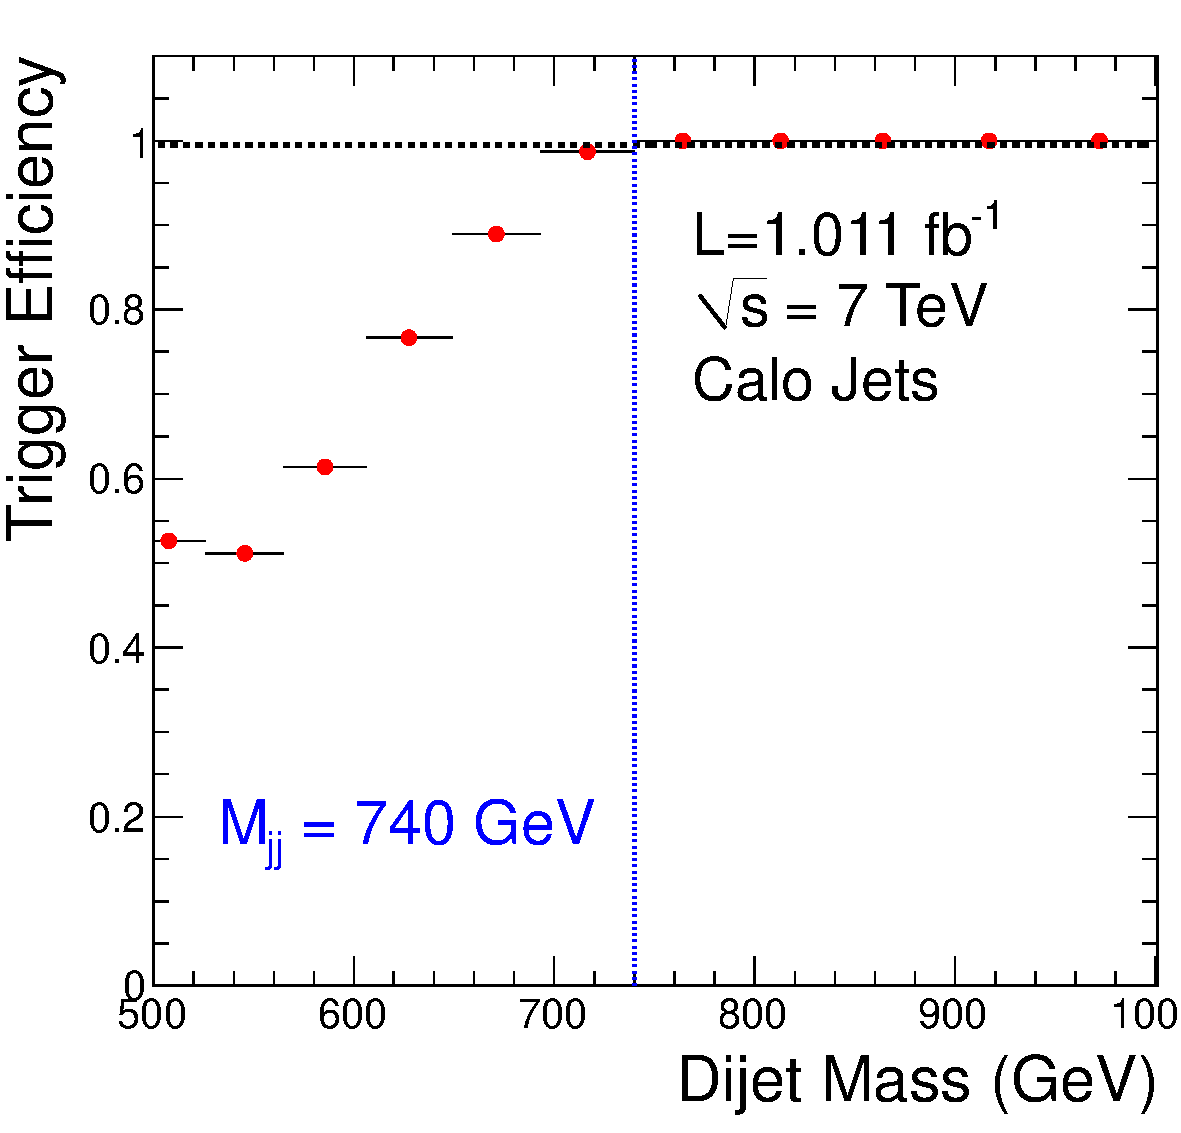
\includegraphics[width=0.45\textwidth]{Figures/trigger_efficiency_1.pdf}
    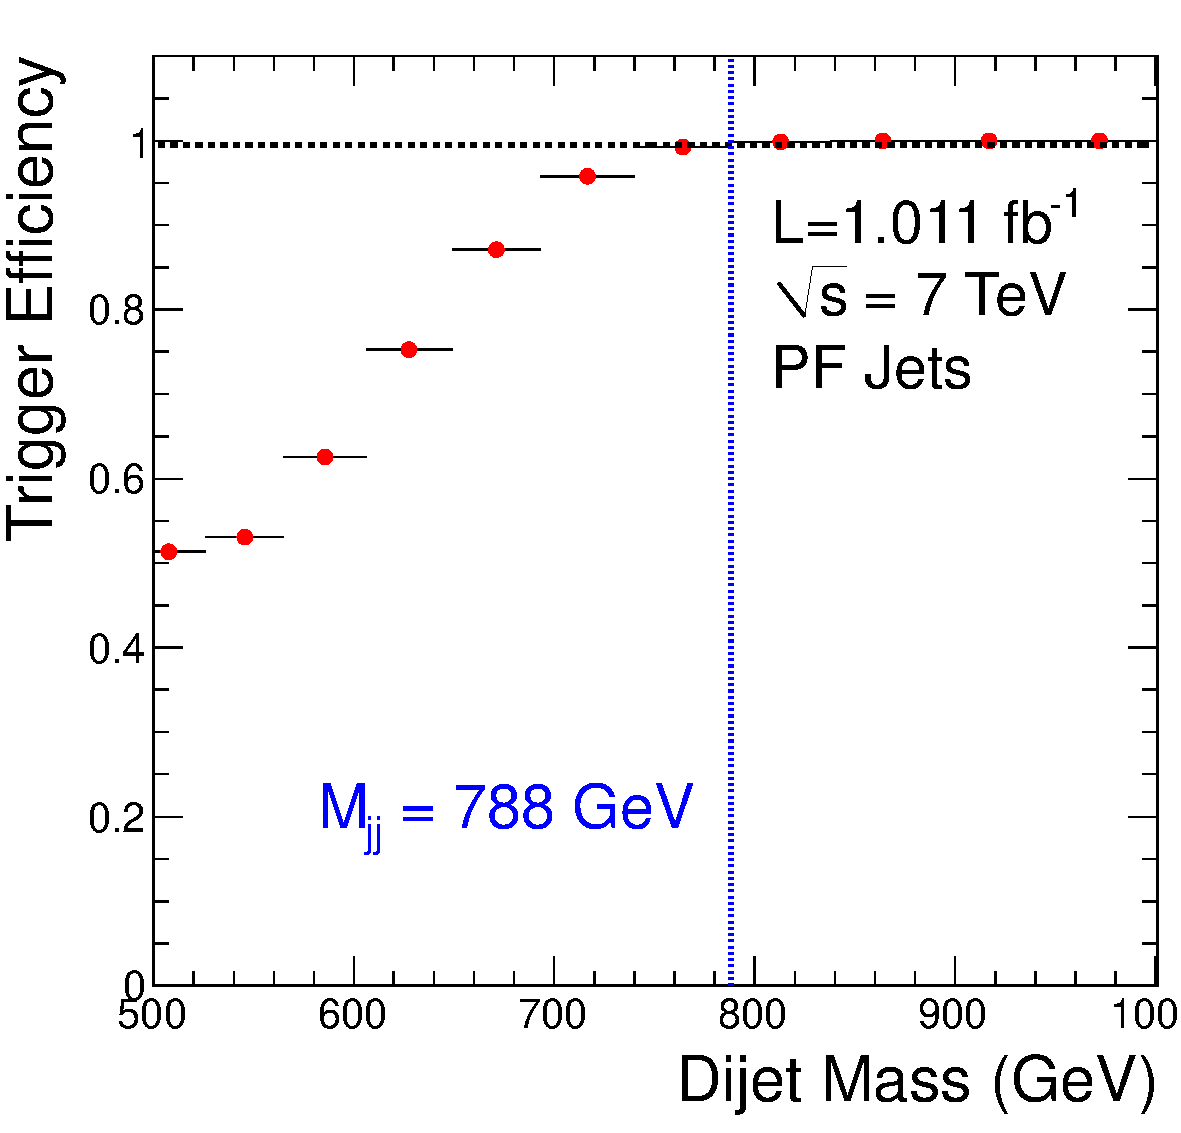
\includegraphics[width=0.45\textwidth]{Figures/trigger_efficiency_2.pdf}
    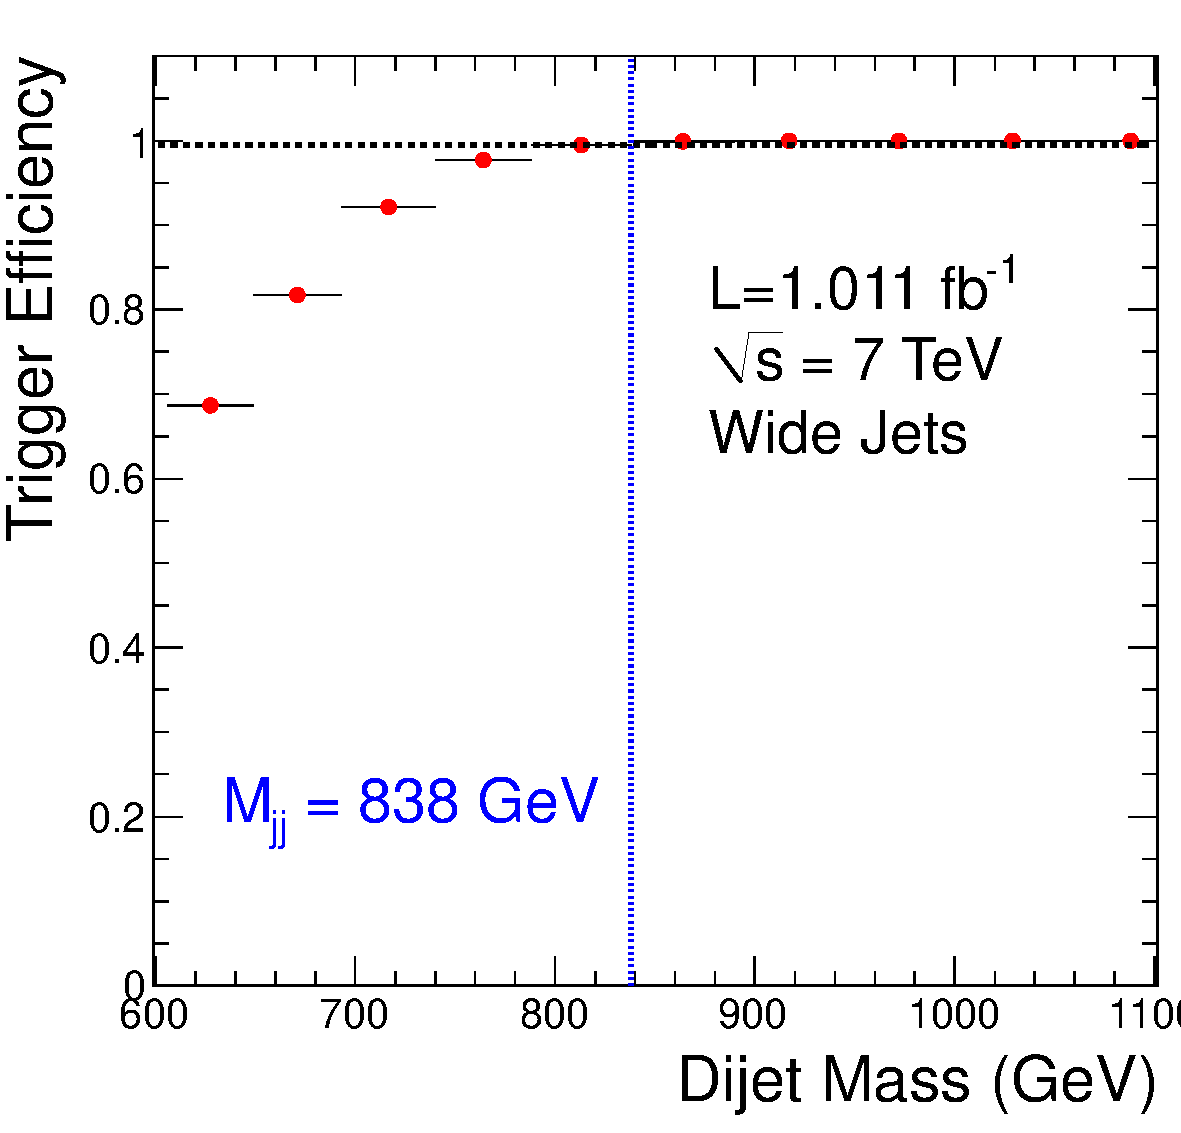
\includegraphics[width=0.45\textwidth]{Figures/trigger_efficiency_3.pdf}
    \caption{ HLT\_HT550 trigger efficiency as a function of dijet mass for 
    $|\eta|<2.5$ and $|\Delta\eta|<1.3$ is measured from the data for Calo jets (top left)
      and PF jets (top right) and efficiency of HT500 trigger for wide Jets (bottom).}
    \label{Trigger}
  \end{center}
\end{figure}

The number of events vs. dijet mass are shown in Fig.~\ref{MassCut}.
The trigger turn-over of the HLT\_Jet500\_v3, HLT\_Jet500\_v4, HLT\_Jet500\_v5,
HLT\_Jet500\_v6, HLT\_Jet500\_v7 trigger can be seen in the mass spectrum
along with the 99.5\% efficiency point at a mass of 838 GeV.

\begin{figure}[!ht]
  \begin{center}
    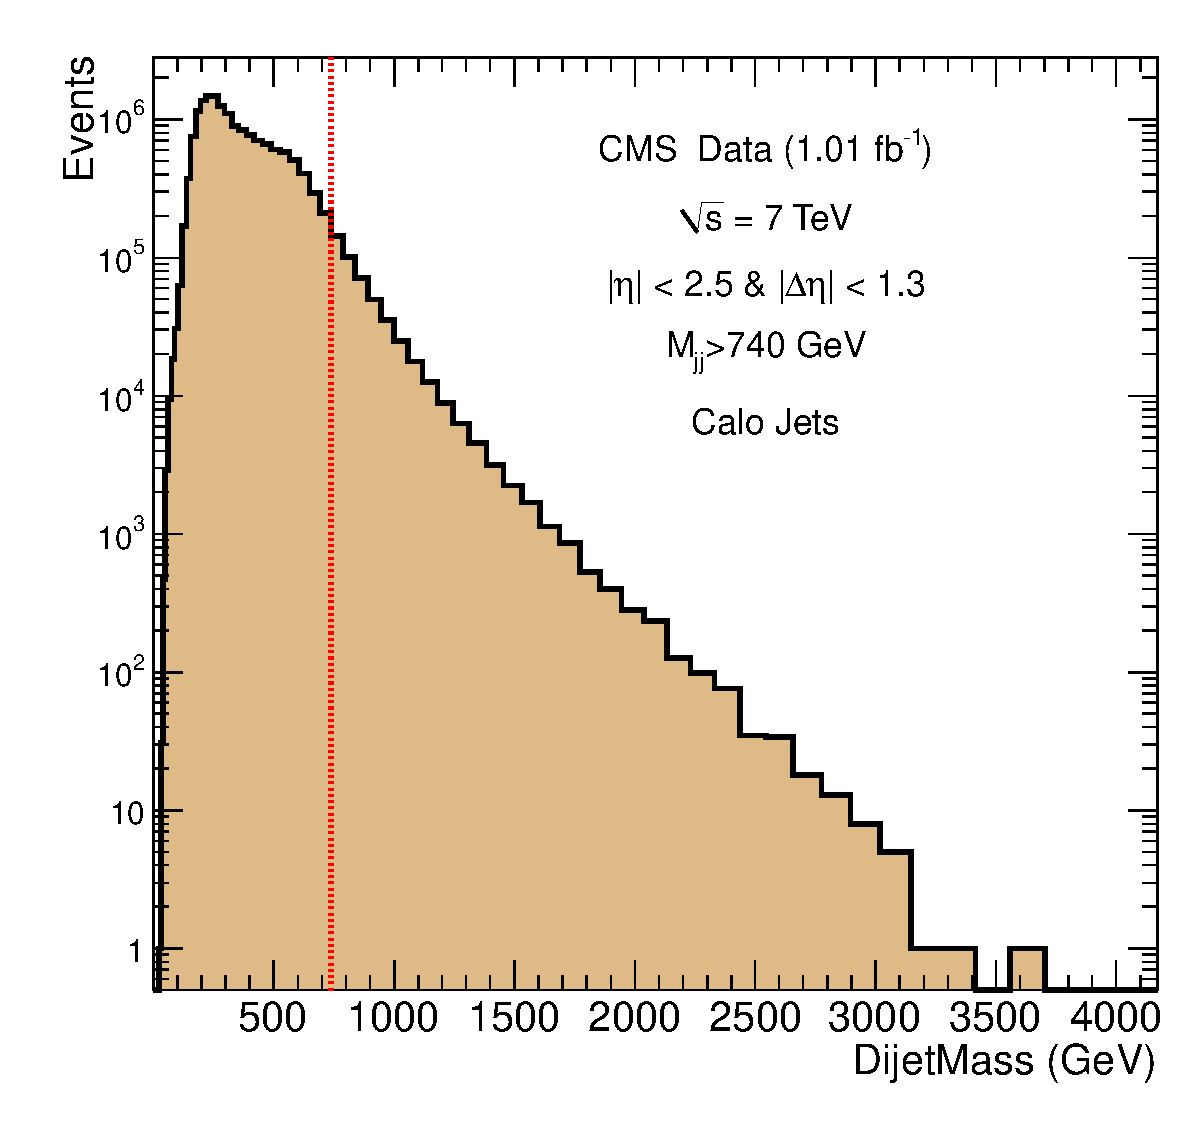
\includegraphics[width=0.45\textwidth]{Figures/c_TurnOver_calo.pdf}
    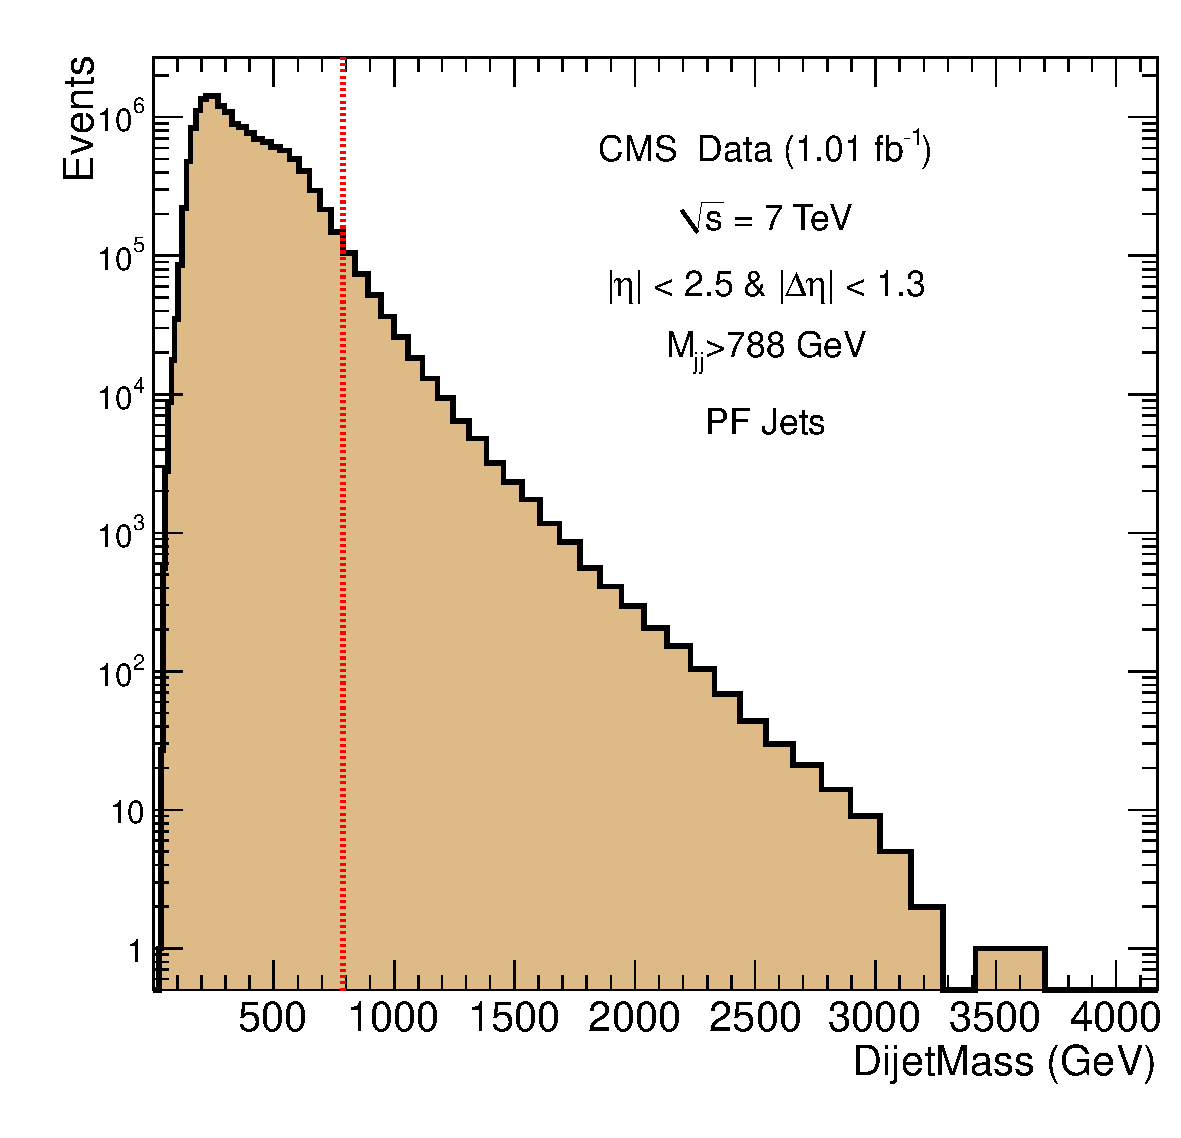
\includegraphics[width=0.45\textwidth]{Figures/c_TurnOver_pf.pdf}
    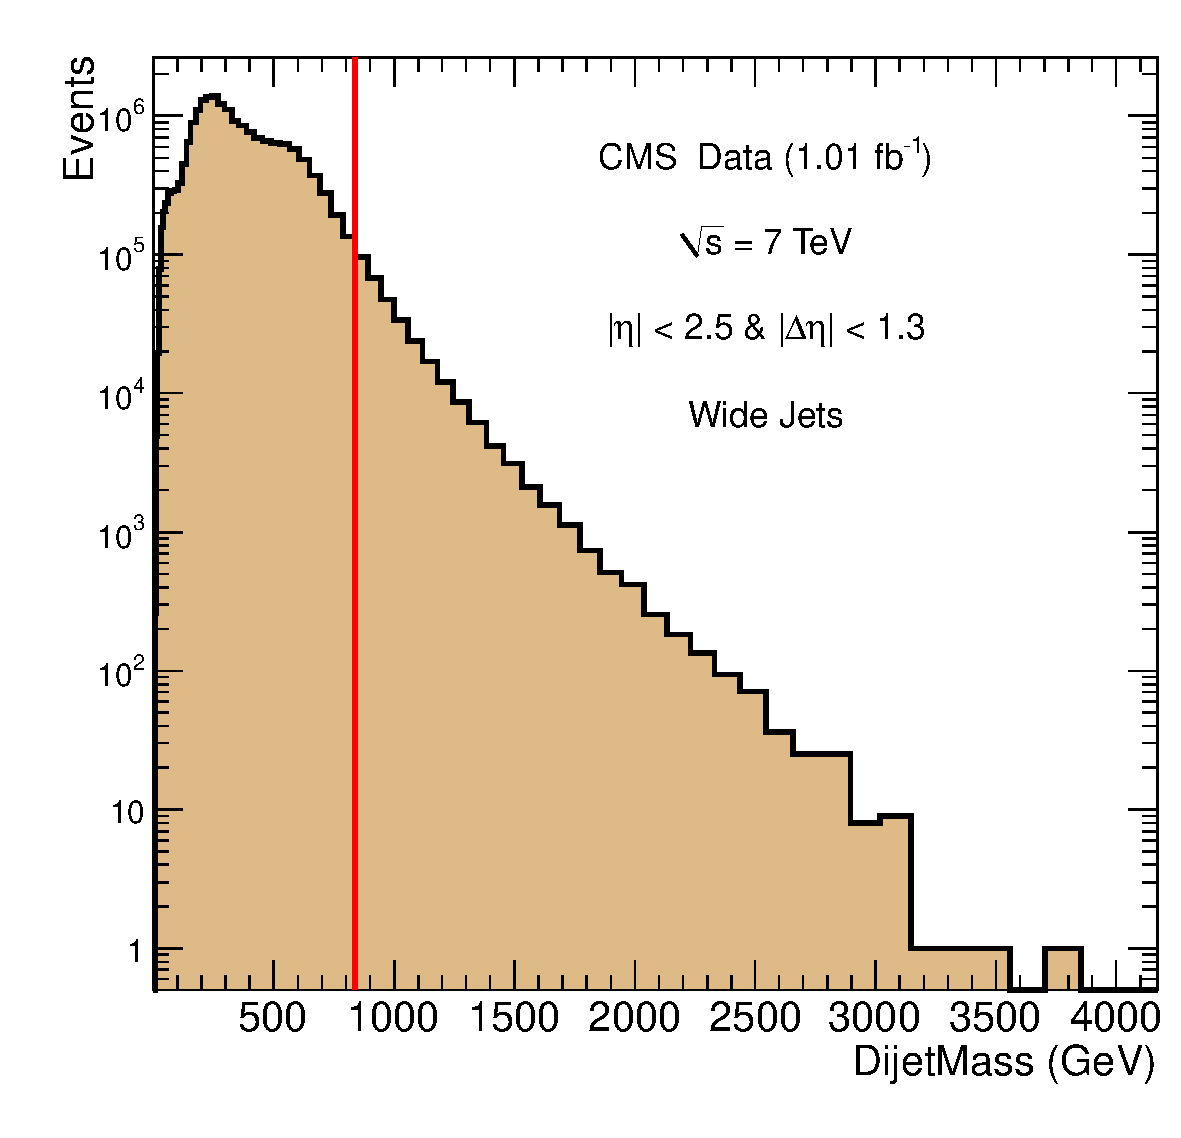
\includegraphics[width=0.45\textwidth]{Figures/c_TurnOver_fat.pdf}
   \caption{ Number of events vs. dijet mass in GeV (histogram)
   requiring all cuts except the final dijet mass cut for trigger
   efficiency at $m=838$ GeV (vertical line). - Calo Jet(top left), PF Jet(top right), Wide Jet(bottom) }.
    \label{MassCut}
  \end{center}
\end{figure}
\clearpage
\subsubsection{Dijet Data Quality}

The number of events in the analysis after the basic cuts are shown for
each cut in table~\ref{table:cuts}
\begin{table}[th]
  \centering
  \normalsize
  \begin{tabular}{|l|r|}
    \hline
    \hline
    Events after vertex cut                              &  7656553\\
    Events after dijet $\eta$ cuts: $|\Delta\eta|<1.3$ and $|\eta|<2.5$ & 2503501\\
    Events after dijet mass cut: $m>838$ GeV             & 320103\\
    Events after jet id cut                              & 319282\\
    \hline
    Events after vertex cut                              &  8196047\\
    Events after dijet $\eta$ cuts: $|\Delta\eta|<1.3$ and $|\eta|<2.5$ & 2074521\\
    Events after dijet mass cut: $m>838$ GeV & 348053\\
    Events after jet id cut                              & 346573\\
    \hline
    Events after vertex cut                              &  8196047\\
    Events after dijet $\eta$ cuts: $|\Delta\eta|<1.3$ and $|\eta|<2.5$ & 2070995\\
    Events after dijet mass cut: $m>838$ GeV & 476366\\
    Events after jet id cut                              & 474872\\
    \hline
  \end{tabular}
  \caption{Cuts and Events for Wide Jet (top), PF Jet (middle), Calo Jet (Bottom)}
  \label{table:cuts}
\end{table}

The fraction of events rejected by jet ID criteria is very small,
because the requirement that the two leading jets have a dijet mass
$m>838$ GeV, $|\eta|<2.5$ and $|\Delta\eta|<1.3$ enhances the jet
purity.  699 events are rejected by calo jet ID and 322 events by PF
Jet ID.

%We have scanned all events rejected by Jet ID that have a
%dijet mass of greater than 2.149 TeV, and they are all HPD noise that
%also has high $MET$, except for one event with scalar sum $\Sigma E_T$
%of 416 TeV uniformly distributed across the HCAL.

%One event rejected by jet ID (run 139407 event 1102912914) has a jet with EMF of 0.009, but otherwise appears to be a good event with
%a dijet mass of $0.5$ TeV.
%One event rejected by Jet ID was in Event 156365648 in Run 135149, noise in a single RBX giving 
%two neighboring jets with EMF of 0 an event MET/$\Sigma E_T$=0.95. 
%A second event rejected by Jet ID was Event 217914565 in Run 135528, noise in  a single HPD,
%again giving two neighboring jets with EMF of 0 and fHPD of 1 and an event MET/$\Sigma E_T$=0.87.
%A third event rejected by Jet ID was Event 103871079 in Run 135175, in which the leading jet
%failed the EMF cut with $EMF=0.005$, but the event looks like it might be a real dijet event:
%jet 1 $p_T=74$ GeV, jet 2 $p_T=35$ GeV, $M_{JJ}=156.4$ GeV, tracks pointing at both jets, 
%$\Delta\phi=2.7$, and a marginal but passable MET/$\Sigma E_T$=0.24.  

After all cuts, we present some basic distributions indicating jet and
event quality in Fig.~\ref{jet_id_calo}, ~\ref{basic_event_calo} and
~\ref{jet_kinematics_calo}.

In Fig.~\ref{jet_id_calo} we show the distributions of the variables of
loose jet ID after all other cuts.  Jet EMF, the fraction of jet
energy in the ECAL, does not have a peak near either zero or one which
would indicate a problem from the HCAL or ECAL. Loose jet ID requires
jet EMF$ > 0.01$ and we find that the cut rejects no real jets in
dijet events as discussed above. Jet fHPD, the fraction of jet energy
in the hottest HCAL HPD, does not have a peak near one which would
indicate a problem from HPD noise.  Loose jet ID requires jet fHPD$ <
0.98$.  Jet n90hits, the number of energy ordered HCAL and ECAL
RecHits containing 90\% of the jet energy, does not have a peak near
one which would indicate hot cells in the calorimeter for example from
Ecal spikes.  Loose jet ID requires jet n90hits $> 1$.  Data and MC
have similar shapes and show smoothly varying distributions for jet
EMF, fHPD, and n90hits characteristic of real jets. Note that data has
significantly more pileup than the MC which affects the comparison in
some of the distributions, like n90hits, but do not affect our final analysis
using high pt jets corrected for pileup.
These jet ID
variables give us confidence that the jets in this analysis do not
originate from backgrounds in the calorimeter.

In Fig.~\ref{track_multiplicity} we show the number of good tracks
associated with either of the two leading jets.  Our leading jets
generally have many associated tracks.  Very few of the leading jets,
in both MC and data, have no associated tracks at the calorimeter
face, and there are virtually no leading jets without associated
tracks at the vertex. The track multiplicity distributions do not have
a peak at zero tracks, which would indicate calorimeter backgrounds.
The track multiplicity distribution gives us additional confidence
that the calorimeter jets in this analysis come from pp collisions.
Note that data has
significantly more pileup than the MC which affects the track multiplicity
distribution.

In Fig.~\ref{basic_event_calo} we show some event balance distributions.
The dijet events have low MET/$\Sigma E_T$, the ratio of the magnitude
of the vector and scalar sums of the CaloTowers, indicating that the
event energy is well balanced in the transverse plane.  Large
background from calorimeter noise, beam halo, or cosmic rays will
typically produced large values of MET/$\Sigma E_T$, which we do not
observe in this data.
%The handful of events with MET/$\Sigma E_T>0.45$
%have been scanned, and they all look like good monojet events at dijet
%mass around $0.49-0.64$ TeV, most likely from $W(\mu \nu)$ + jet or
%$Z(\mu\mu, \nu\nu)$ + jet processes.
The two leading jets are predominantly back-to-back in $\phi$ as
expected for dijets, with a tail to small values of $\Delta\phi$ 
produced by radiation and multi-jet events.
Data and MC have similar shapes and show smoothly varying distributions
for MET/$\Sigma E_T$ and $\Delta\phi$ characteristic of dijet events.
Thes distributions give us confidence that we are observing events with
a dijet topology, not unphysical backgrounds.

In Fig.~\ref{jet_kinematics_calo} we show some distributions of basic jet
kinematic variables.  The $p_T$ distribution falls steeply with
increasing $p_T$, and turns over at low $p_T$ due to the dijet mass
cut $m>838$ GeV.  The jet $p_T$ distributions for data and MC are in
good agreement considering uncertainties in the jet energy scale,
and the modelling of the $p_T$
distribution in PYTHIA.  The $\eta$ distribution of the two leading
jets is in reasonable agreement with the shape predicted by the MC,
and there are no regions with significant rate deviations that could
arise due to significant mis-understanding of jet response after all
corrections. The $\Delta\eta$ distribution demonstrates the
characteristic forward peaks from Rutherford-like QCD scattering at
fixed invariant mass, and the very slight deviations in shape between
data and MC are expected from NLO effects on the angular distribution.
The $\phi$ distribution of the two leading jets is flat, with an RMS
of only 2.5\%
%, which corresponds to a CaloJet response which is flat
%as a function of phi to within about 0.4\%. This is reasonable given
%the expected calorimeter response uniformity in $\phi$. 
 The $\eta$ -
$\phi$ distribution of two leading jets is reasonably uniform.
%and does
%not show any indication of hot or dead regions of the calorimeter.
These distributions show that the jets in this data sample have the
kinematics expected for dijets from QCD.

\begin{figure}[!ht]
  \begin{center}
    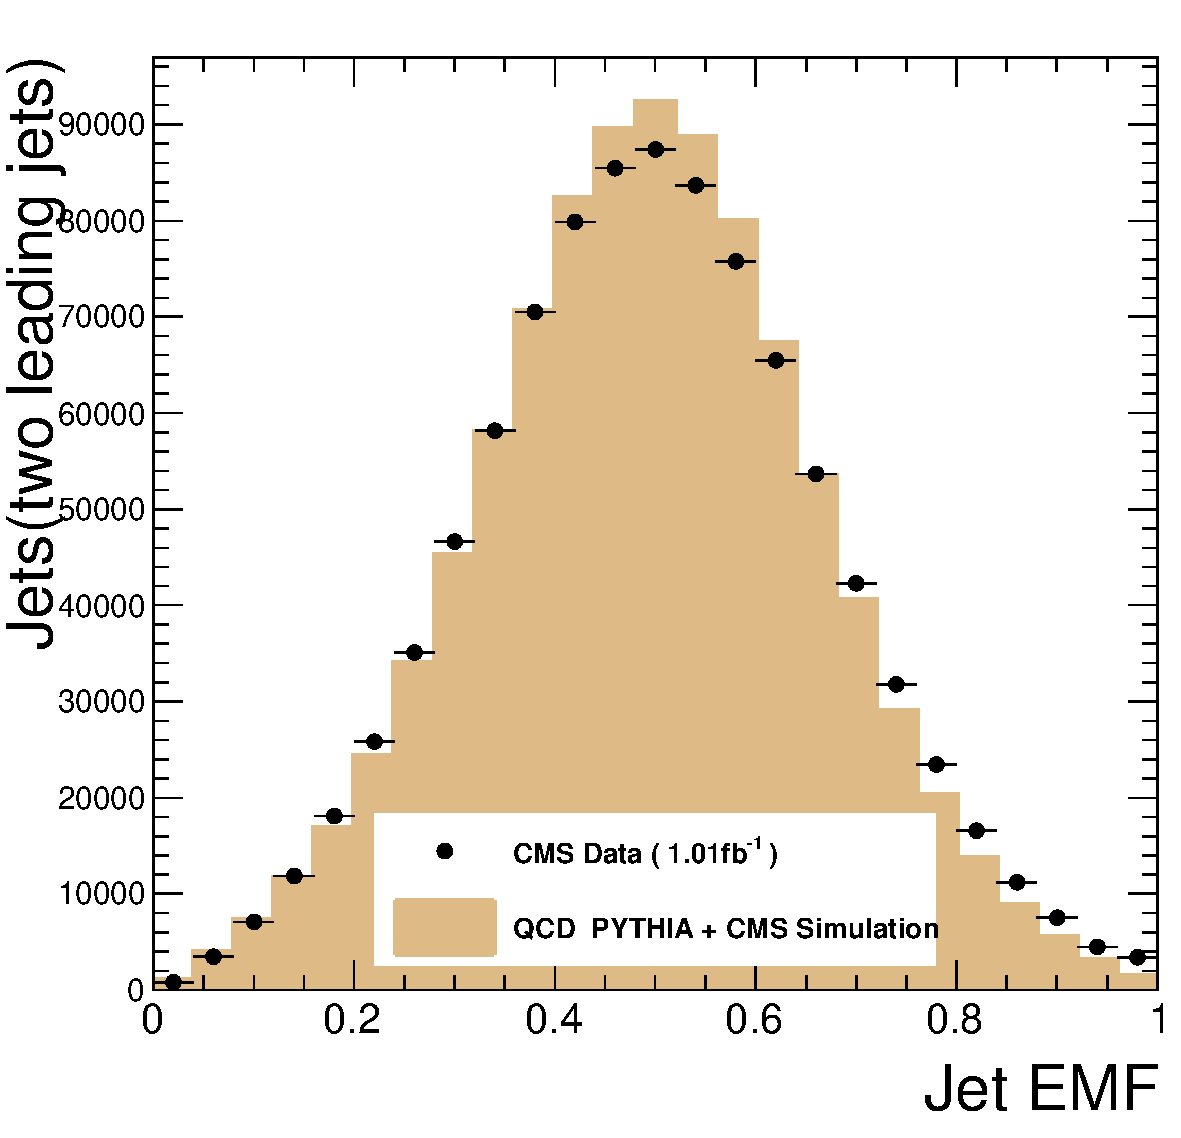
\includegraphics[width=0.45\textwidth]{Figures/c_EMF.pdf}
    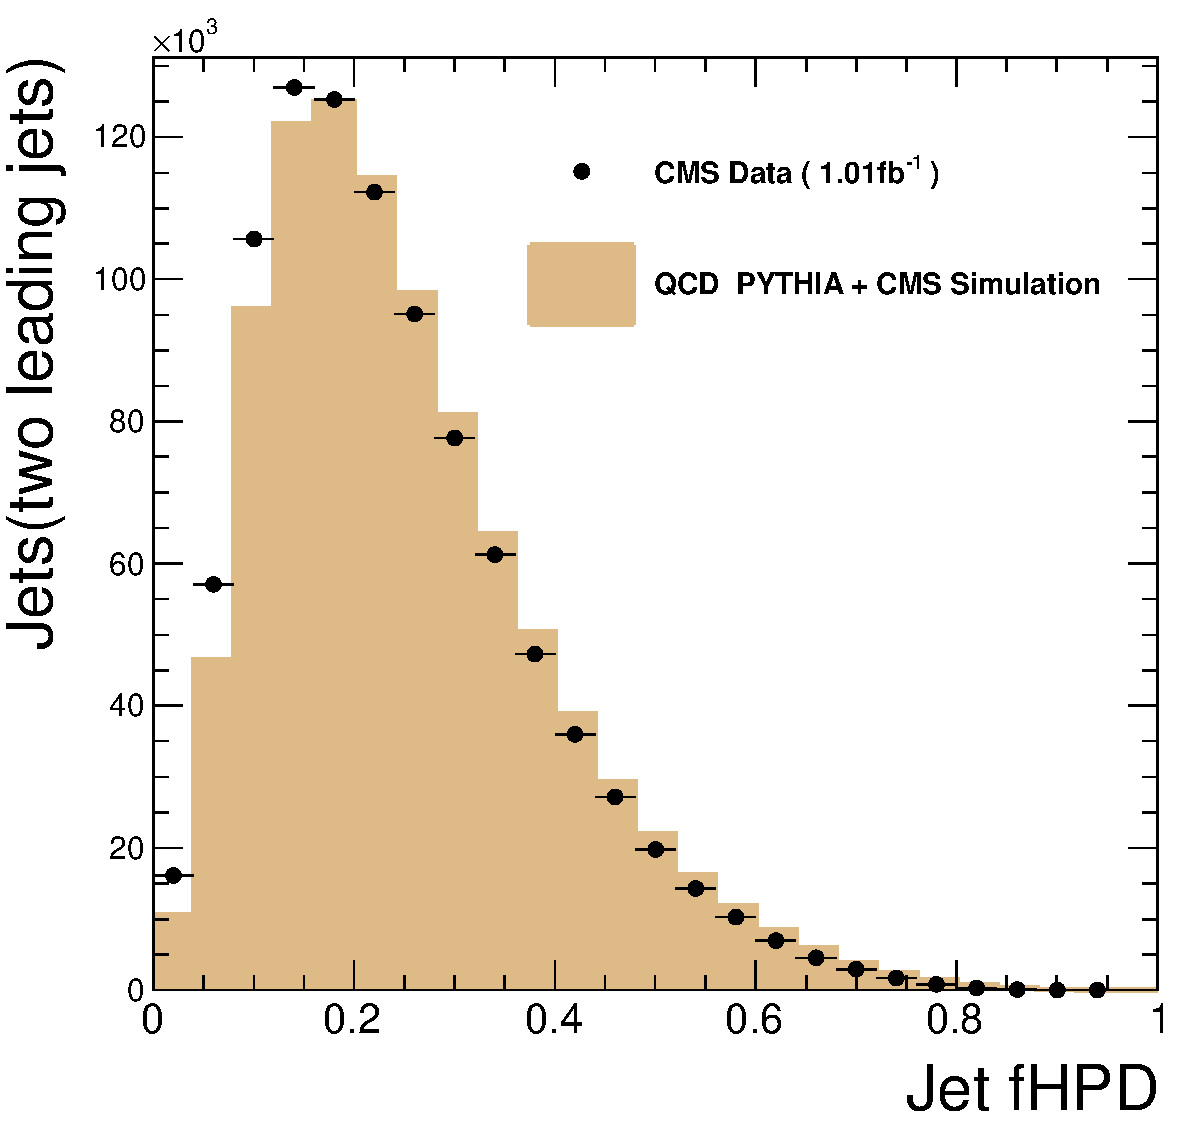
\includegraphics[width=0.45\textwidth]{Figures/c_fHPD.pdf}
    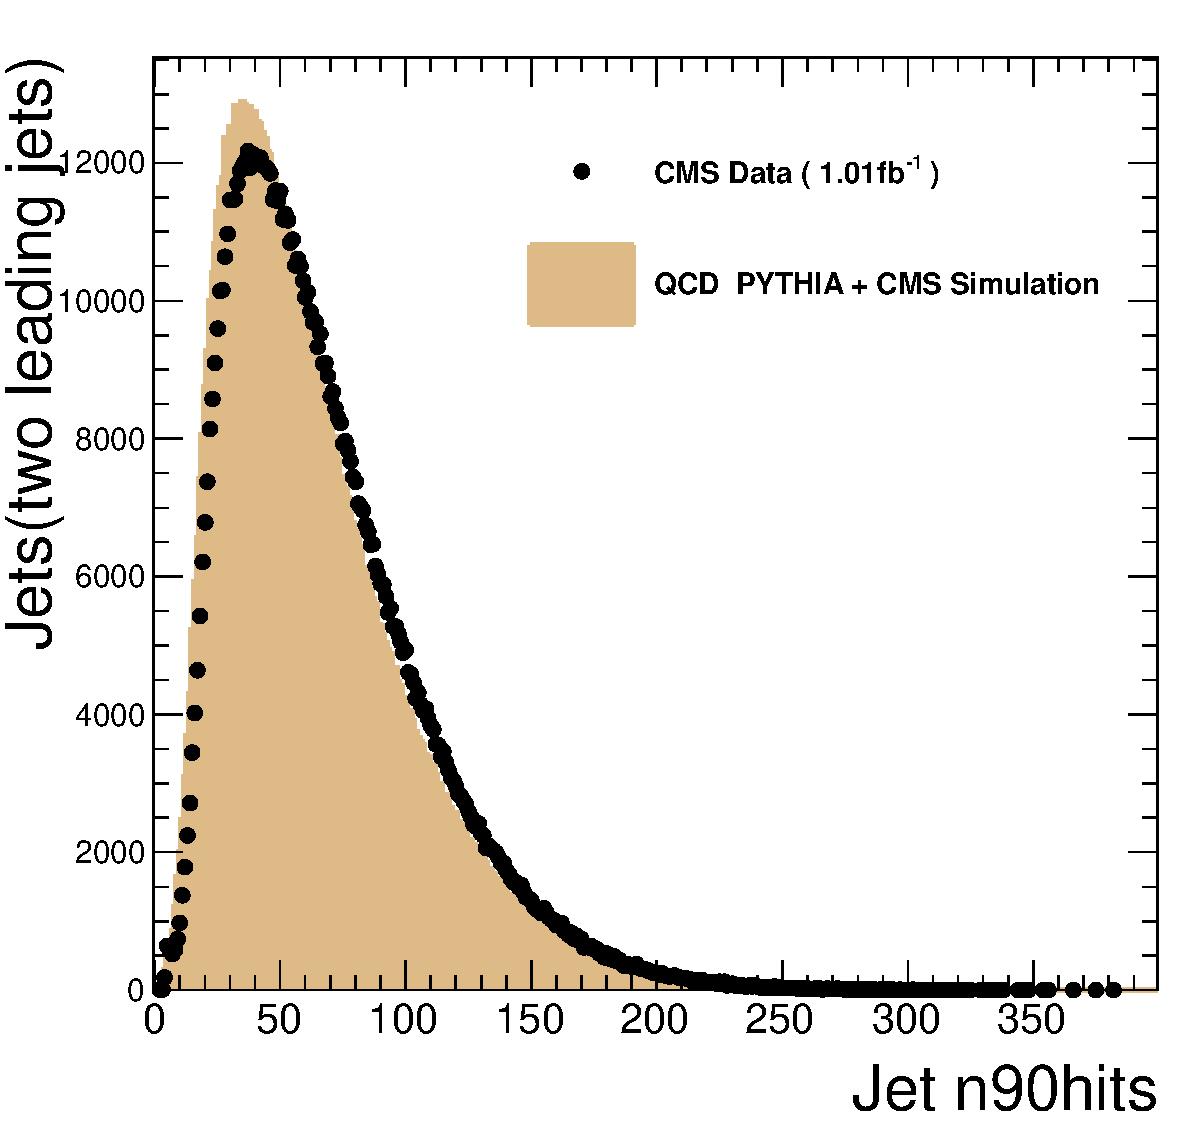
\includegraphics[width=0.45\textwidth]{Figures/c_n90hits.pdf}
    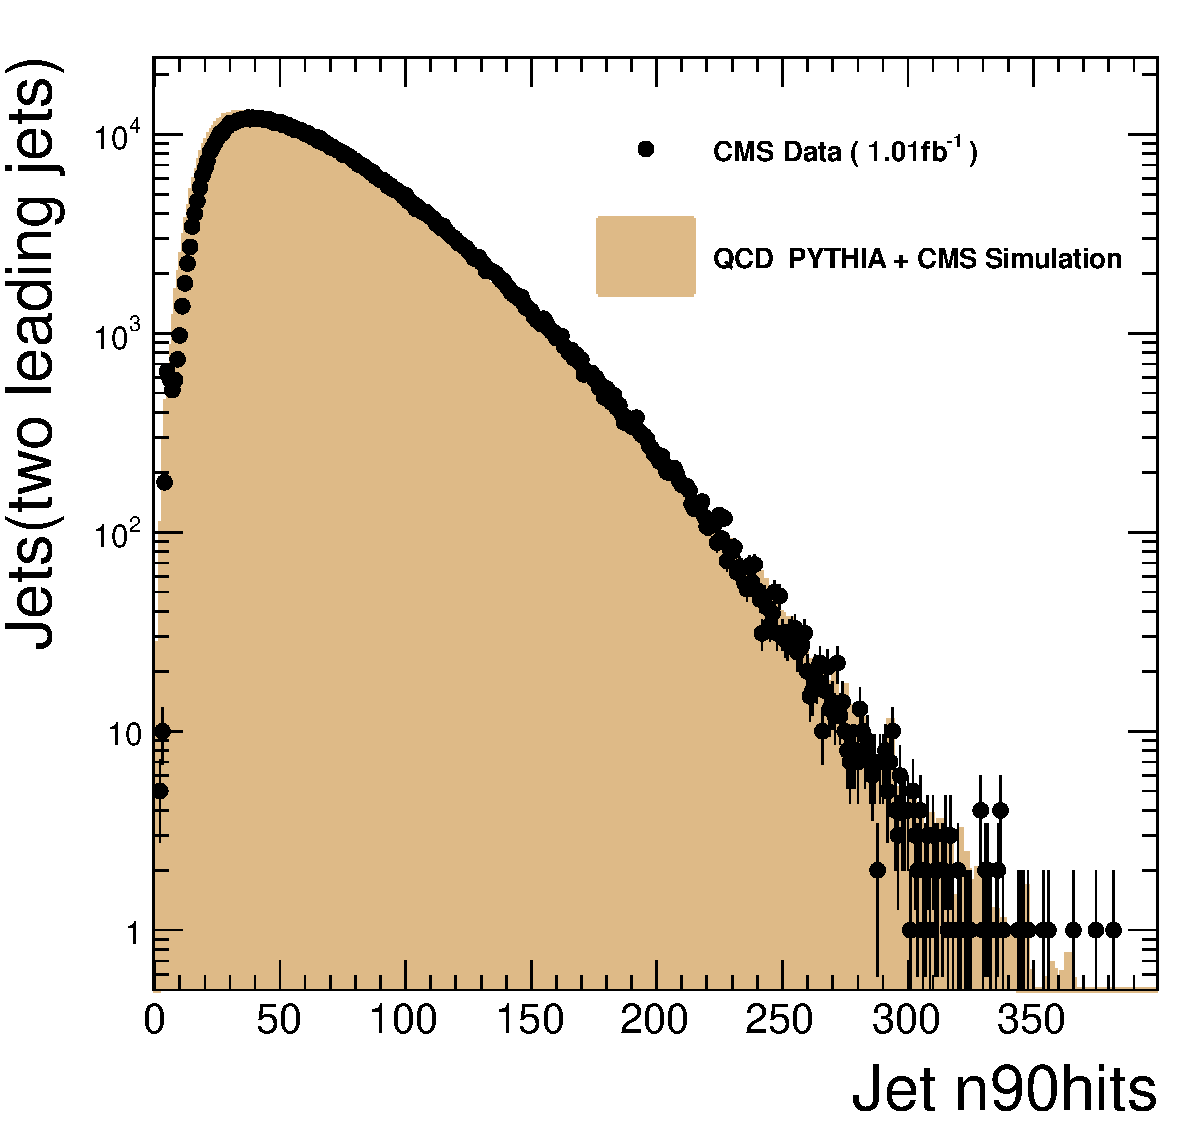
\includegraphics[width=0.45\textwidth]{Figures/c_n90hits_log.pdf}

    \caption{Jet ID Distributions(Calo).  The EM
      energy fraction of the two leading jets (upper left), the fHPD for the two
      leading jets (upper right), the n90hits for the two leading jets
      (lower left) and the same in log scale
      (lower right). }
    \label{jet_id_calo}
  \end{center}
\end{figure}

\begin{figure}[!ht]
  \begin{center}
    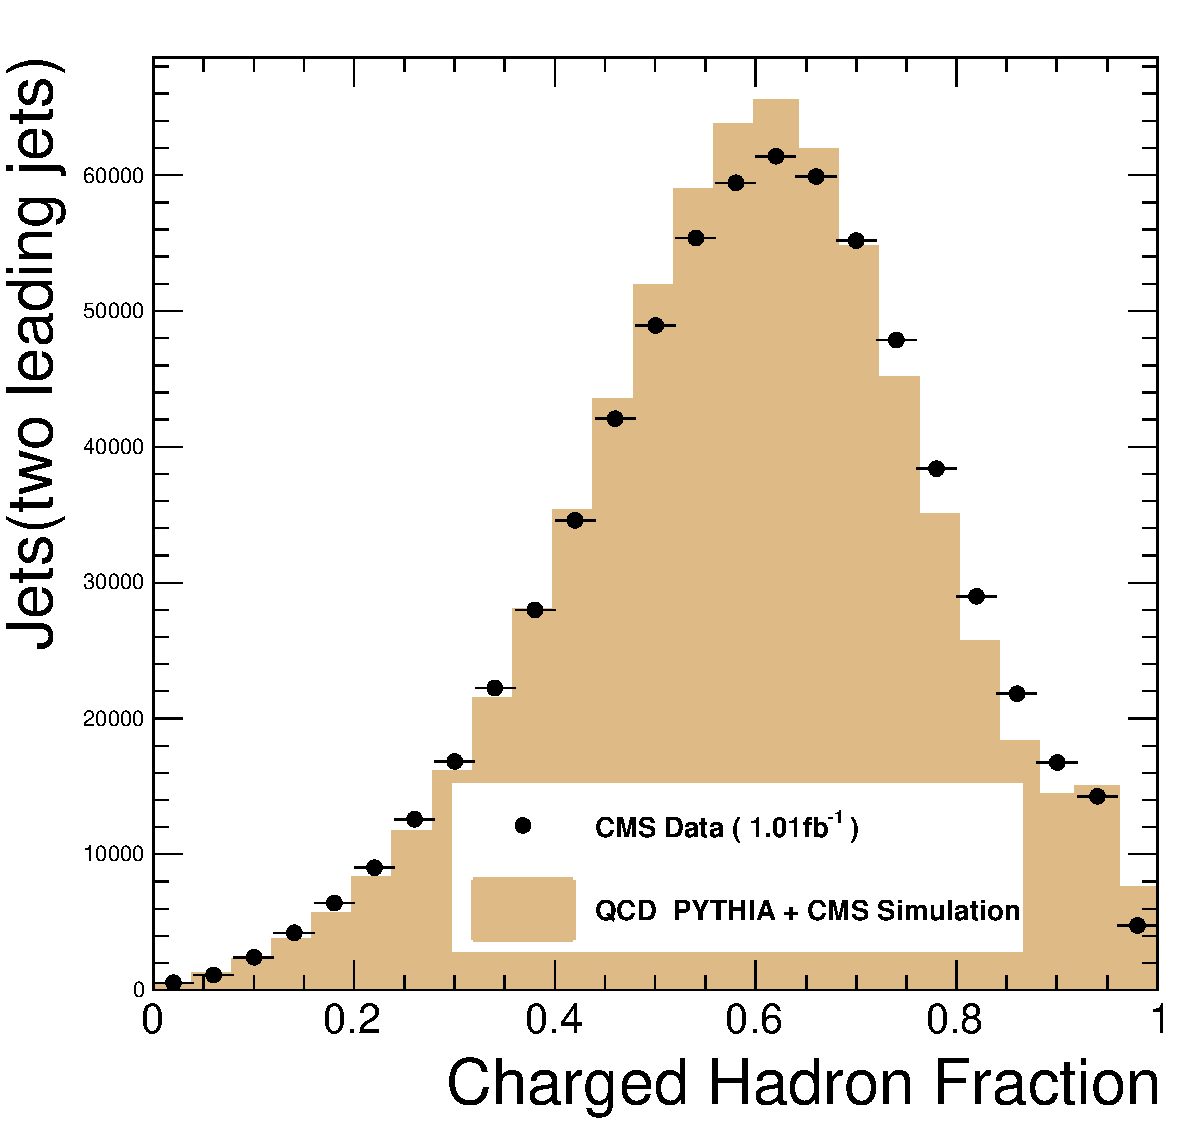
\includegraphics[width=0.45\textwidth]{Figures/c_fCh_pf.pdf}
    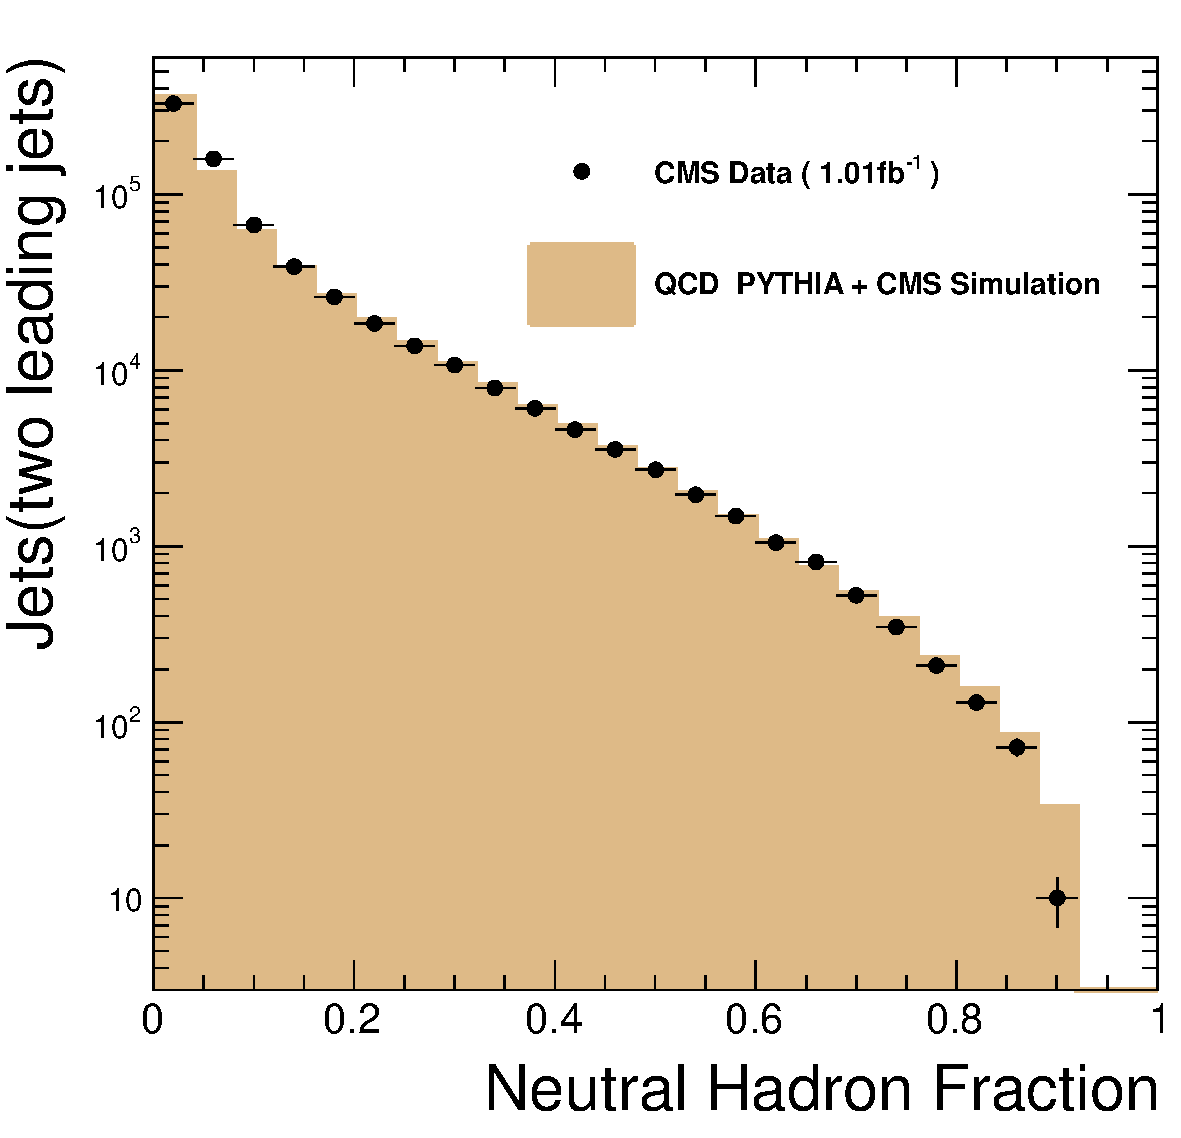
\includegraphics[width=0.45\textwidth]{Figures/c_fNh_pf.pdf}
    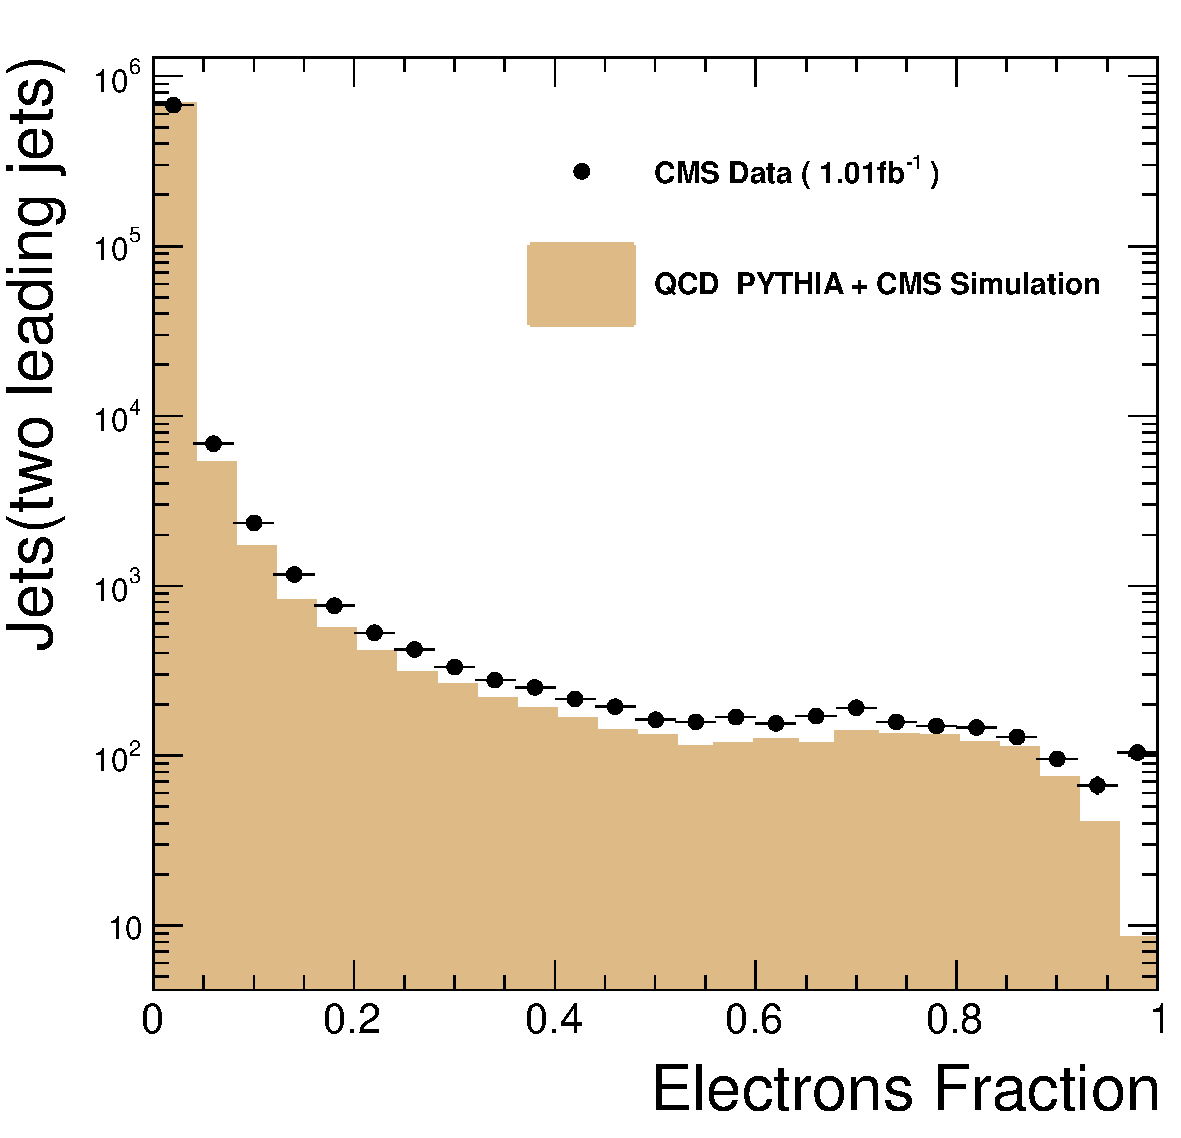
\includegraphics[width=0.45\textwidth]{Figures/c_fEl_pf.pdf}
    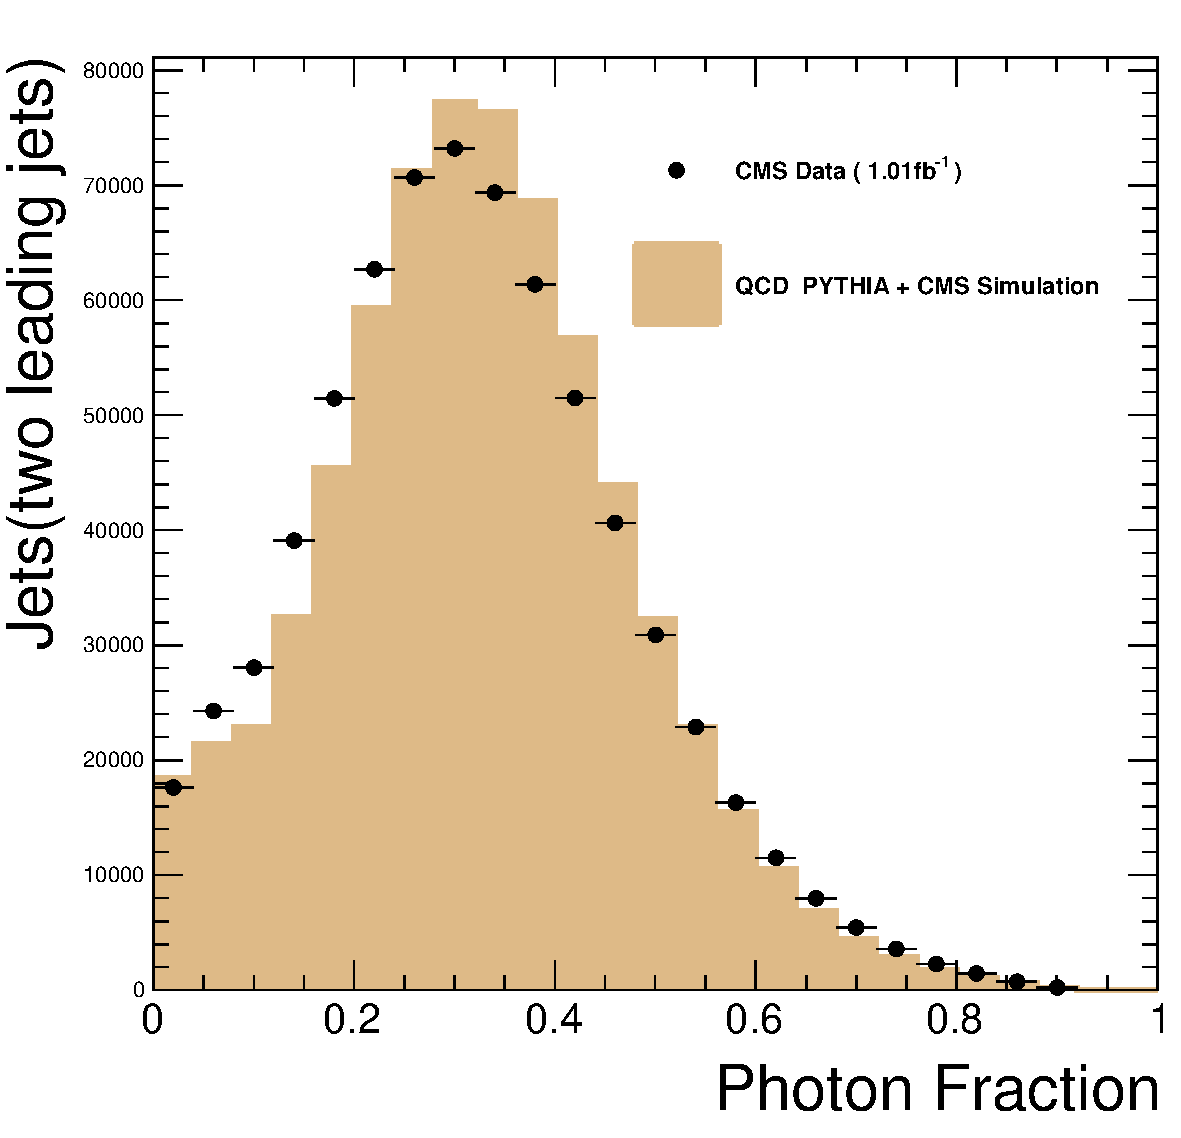
\includegraphics[width=0.45\textwidth]{Figures/c_fPh_pf.pdf}

    \caption{Jet ID Distributions(PF).  The Charged Hadron fraction distribution
      (upper left), the Neutral Hadron Fraction distribution (upper right),
      the electrons fraction distribution in log scale(lower left) and the Photon
      fraction distribution(lower right). }
    \label{jet_id_pf}
  \end{center}
\end{figure}

\begin{figure}[!ht]
  \begin{center}
    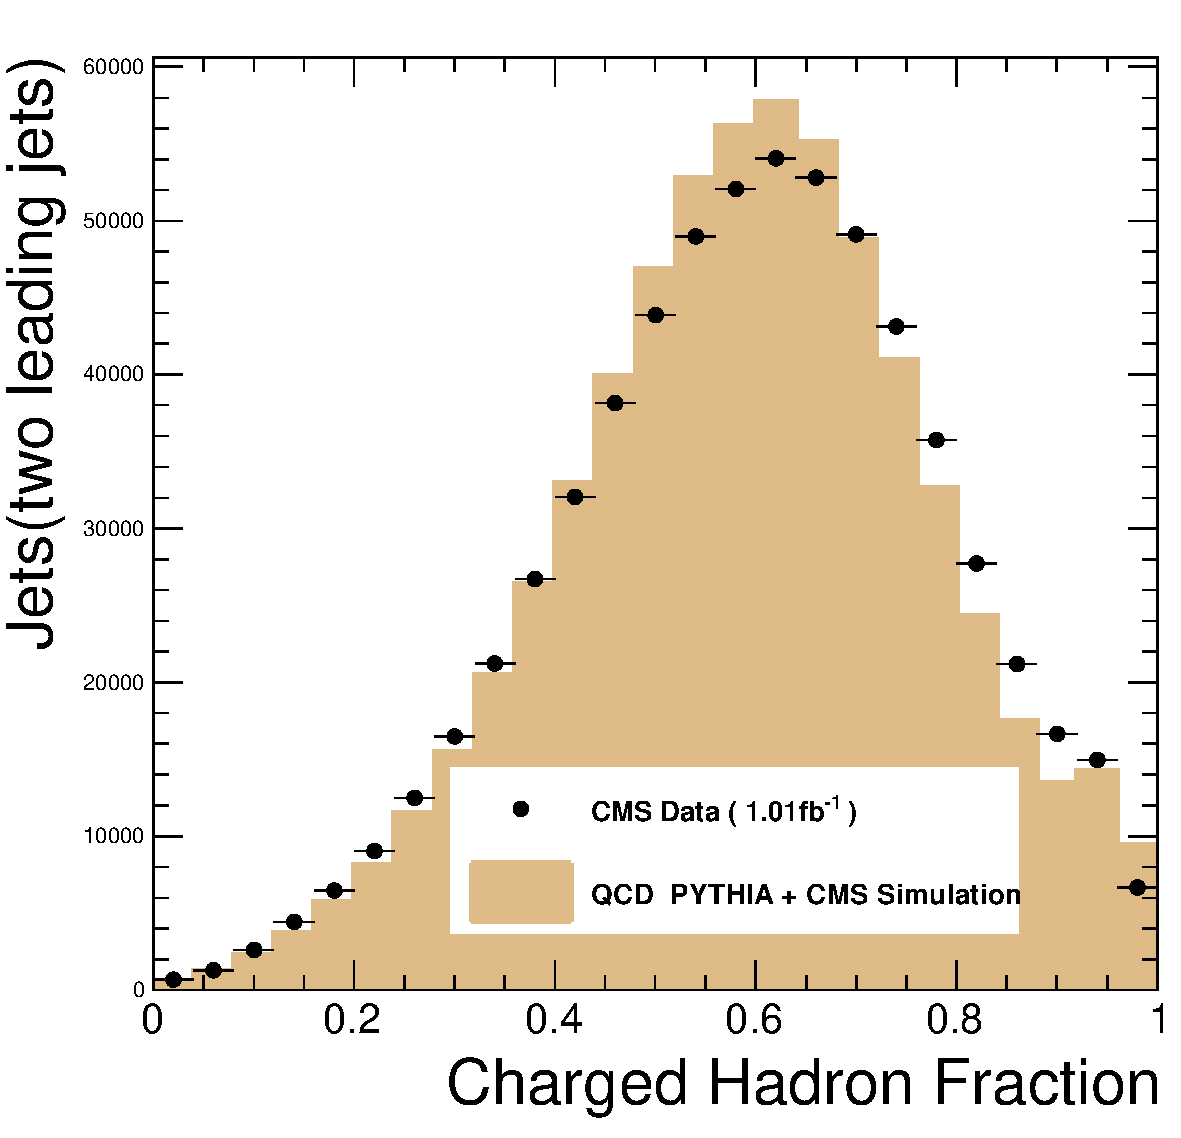
\includegraphics[width=0.45\textwidth]{Figures/c_fCh_fat.pdf}
    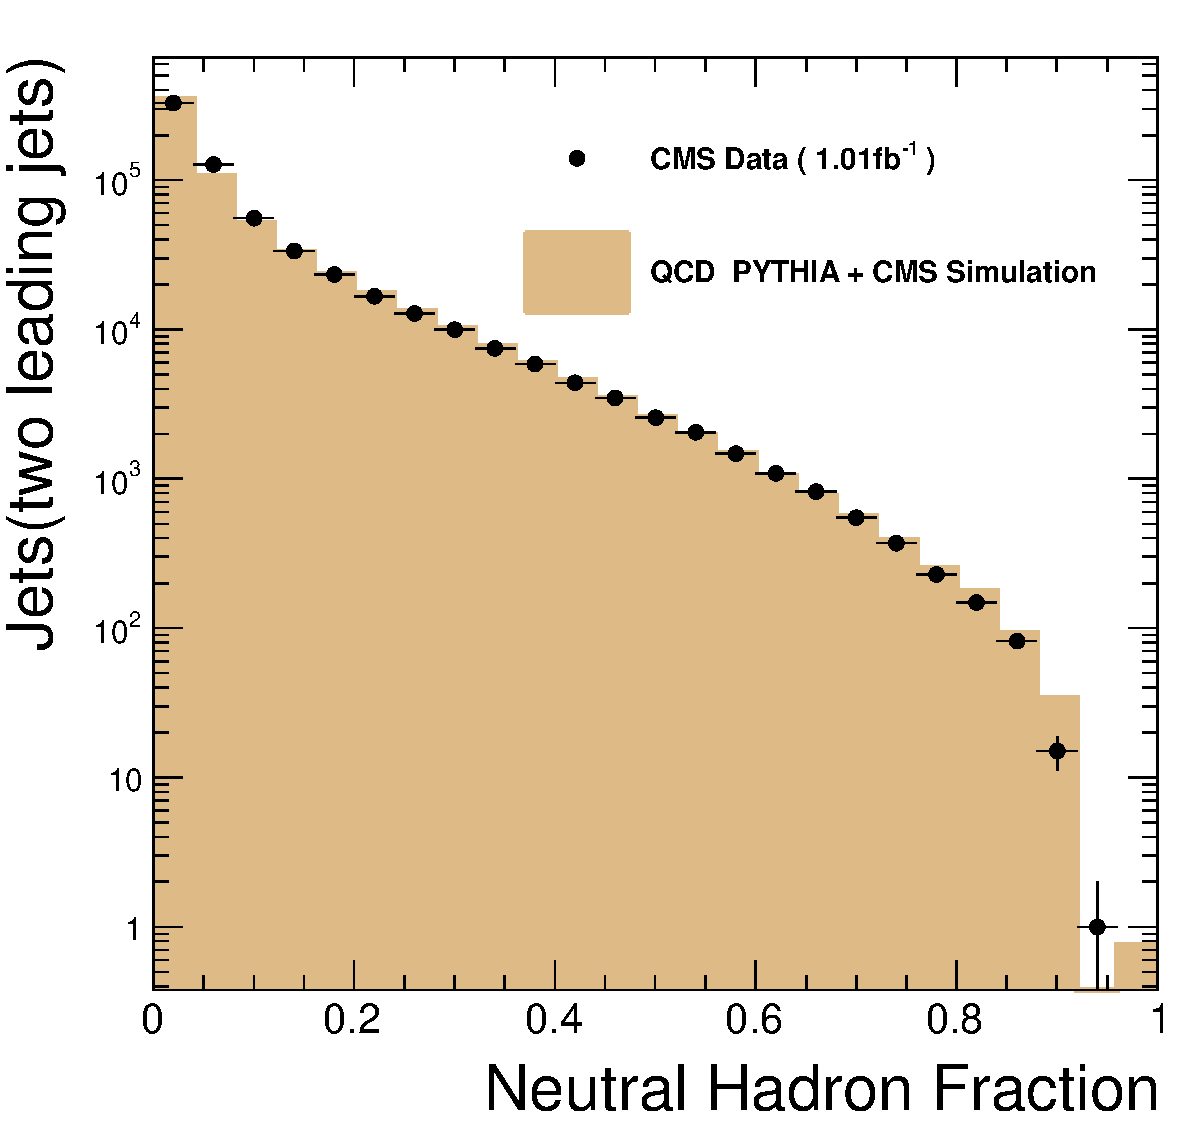
\includegraphics[width=0.45\textwidth]{Figures/c_fNh_fat.pdf}
    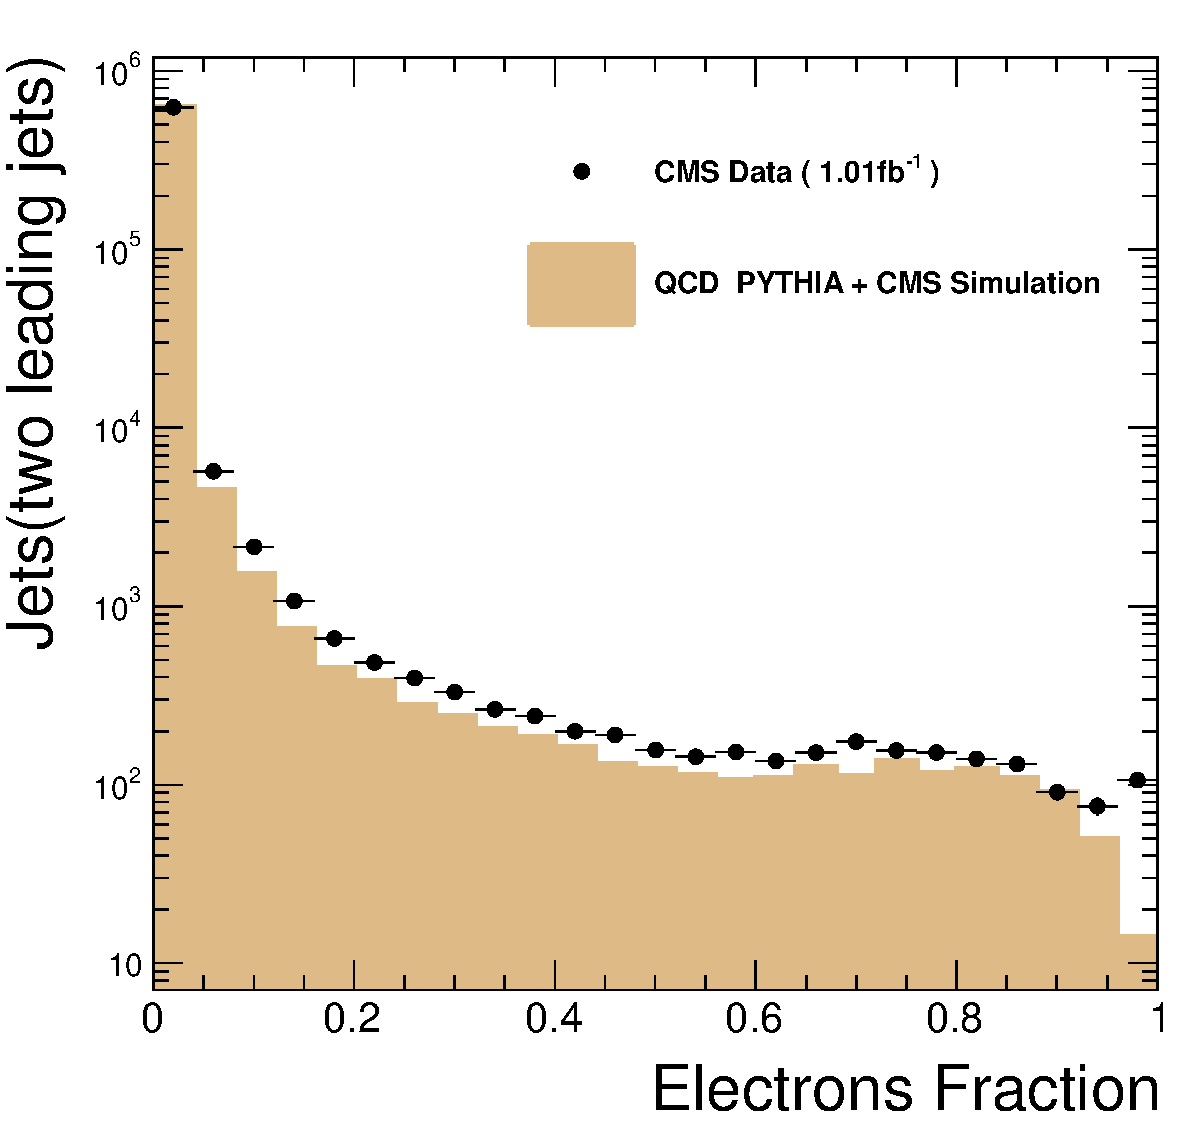
\includegraphics[width=0.45\textwidth]{Figures/c_fEl_fat.pdf}
    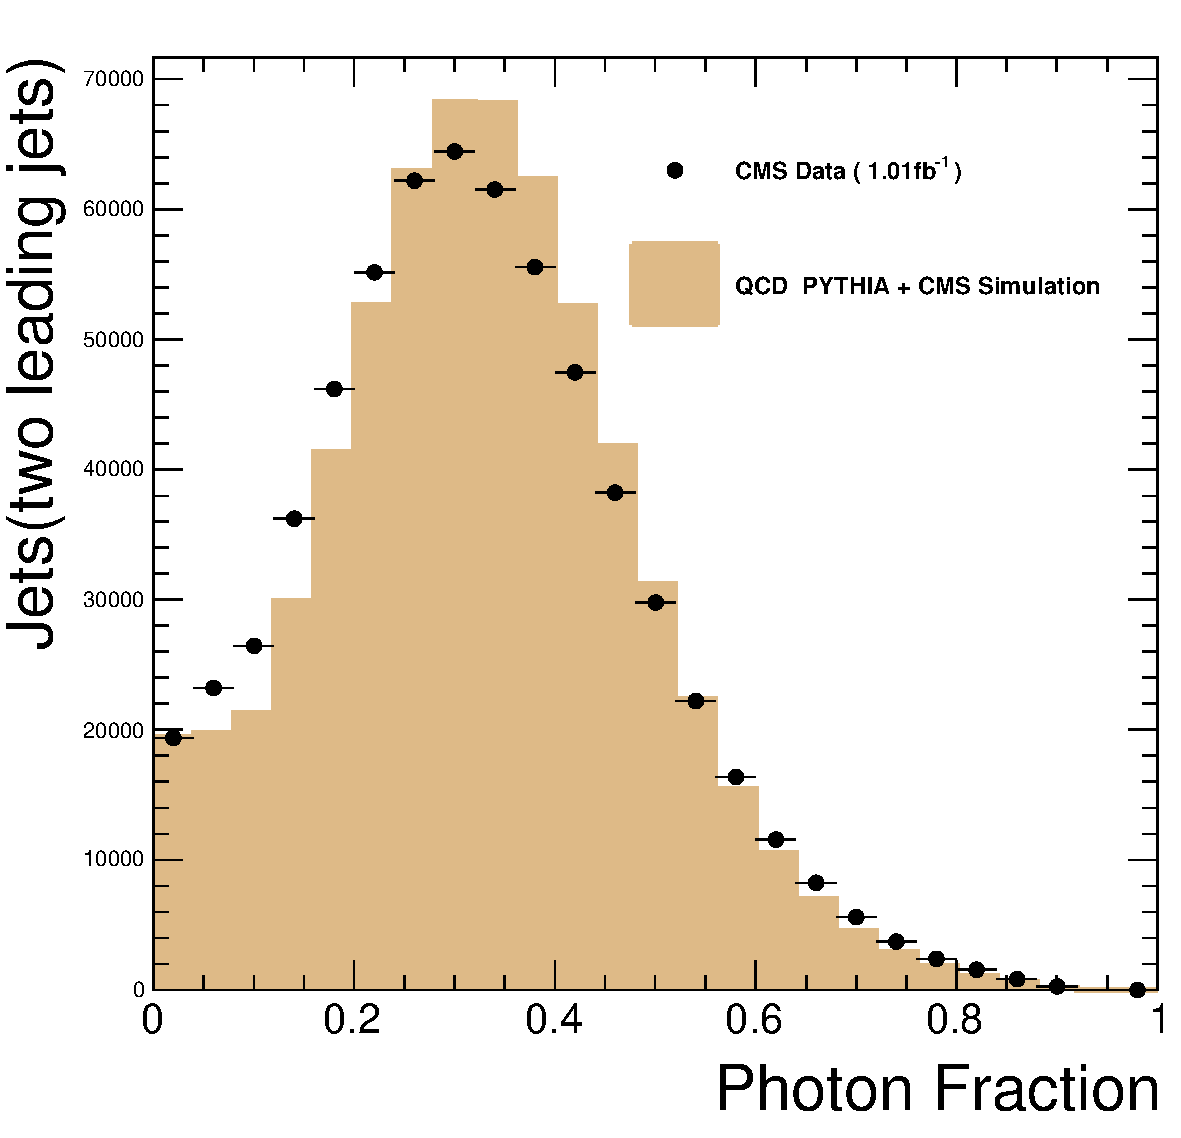
\includegraphics[width=0.45\textwidth]{Figures/c_fPh_fat.pdf}

    \caption{Jet ID Distributions(Wide).  The Charged Hadron fraction distribution
      (upper left), the Neutral Hadron Fraction distribution (upper right),
      the electrons fraction distribution in log scale(lower left) and the Photon
      fraction distribution(lower right). }
    \label{jet_id_wide}
  \end{center}
\end{figure}

\begin{figure}[!ht]
  \begin{center}
    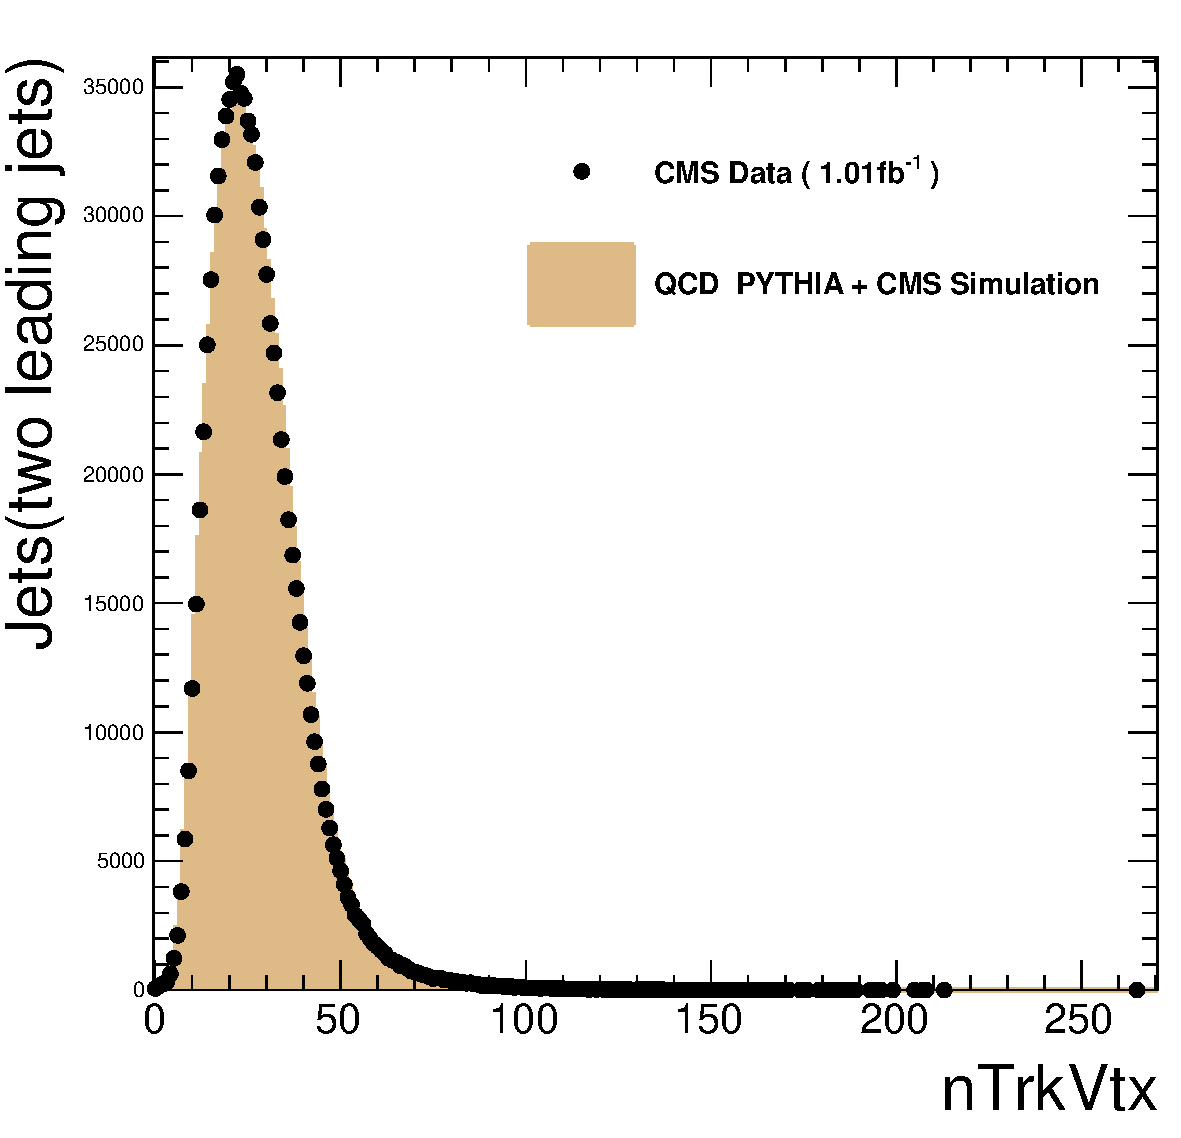
\includegraphics[width=0.45\textwidth]{Figures/c_nTrkVtx.pdf}
    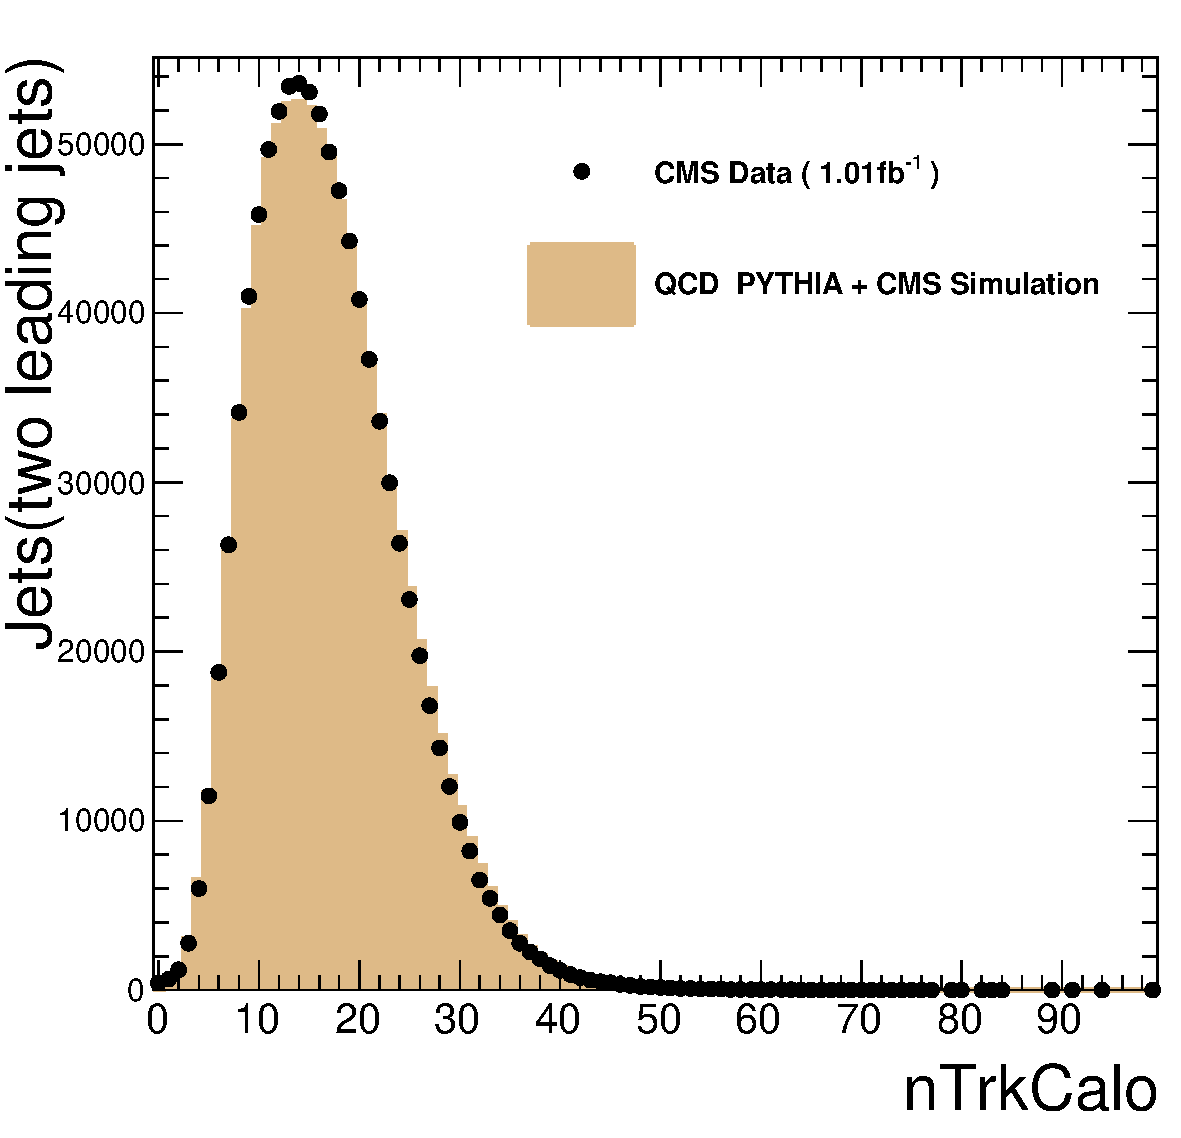
\includegraphics[width=0.45\textwidth]{Figures/c_nTrkCalo.pdf}
    \caption{ left) The multiplicity of tracks associated to two leading jets at the vertex right) The multiplicity of tracks associated to two leading jets at the calo face}
    \label{track_multiplicity}
  \end{center}
\end{figure}

\begin{figure}[!ht]
  \begin{center}
   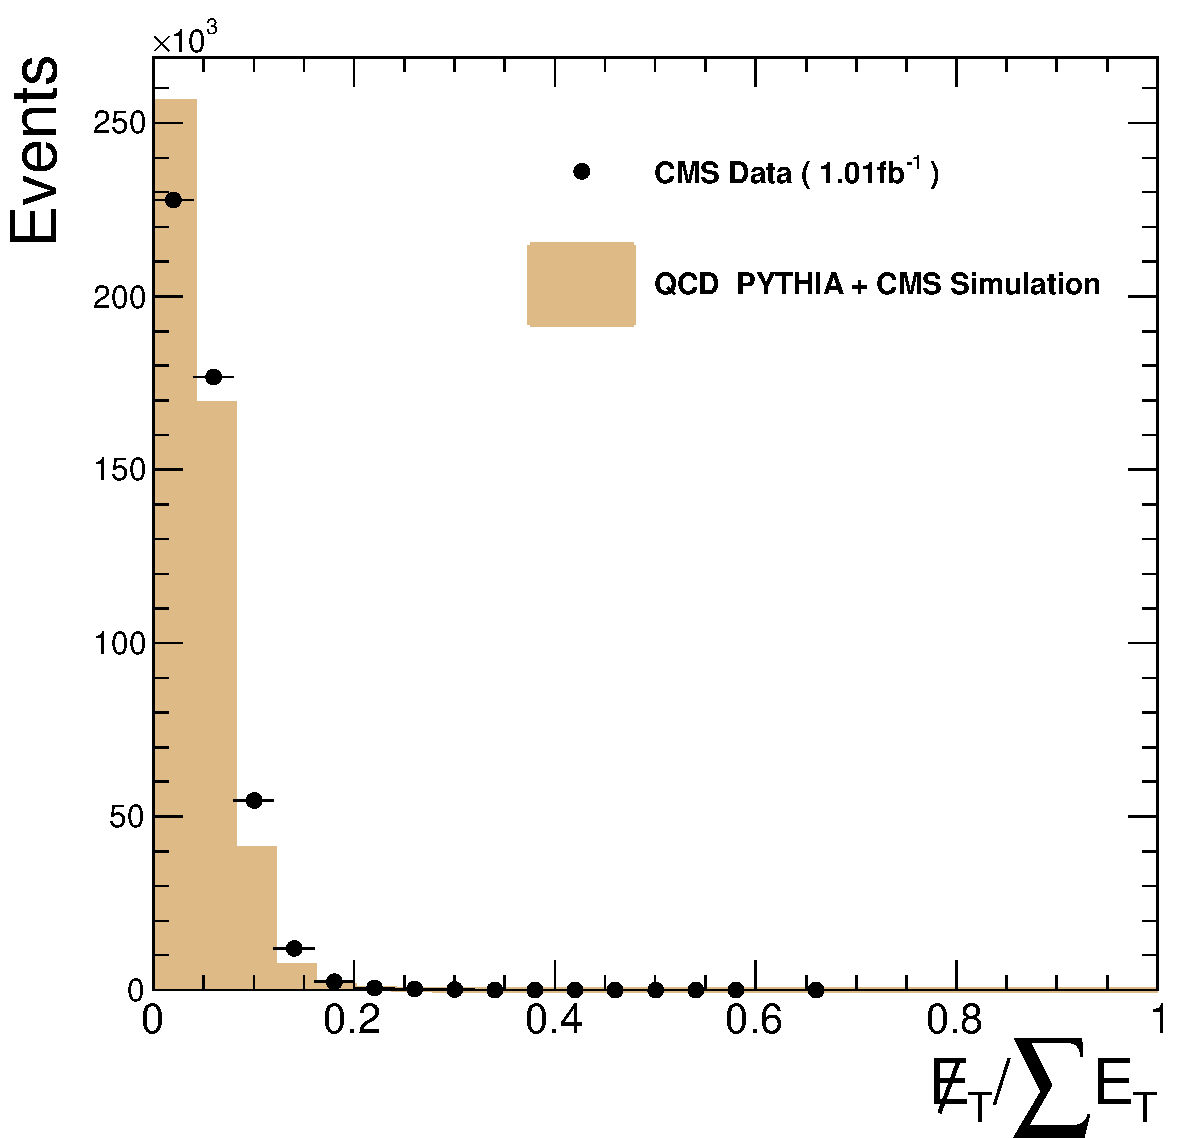
\includegraphics[width=0.45\textwidth]{Figures/c_MET_over_sumEt.pdf}
   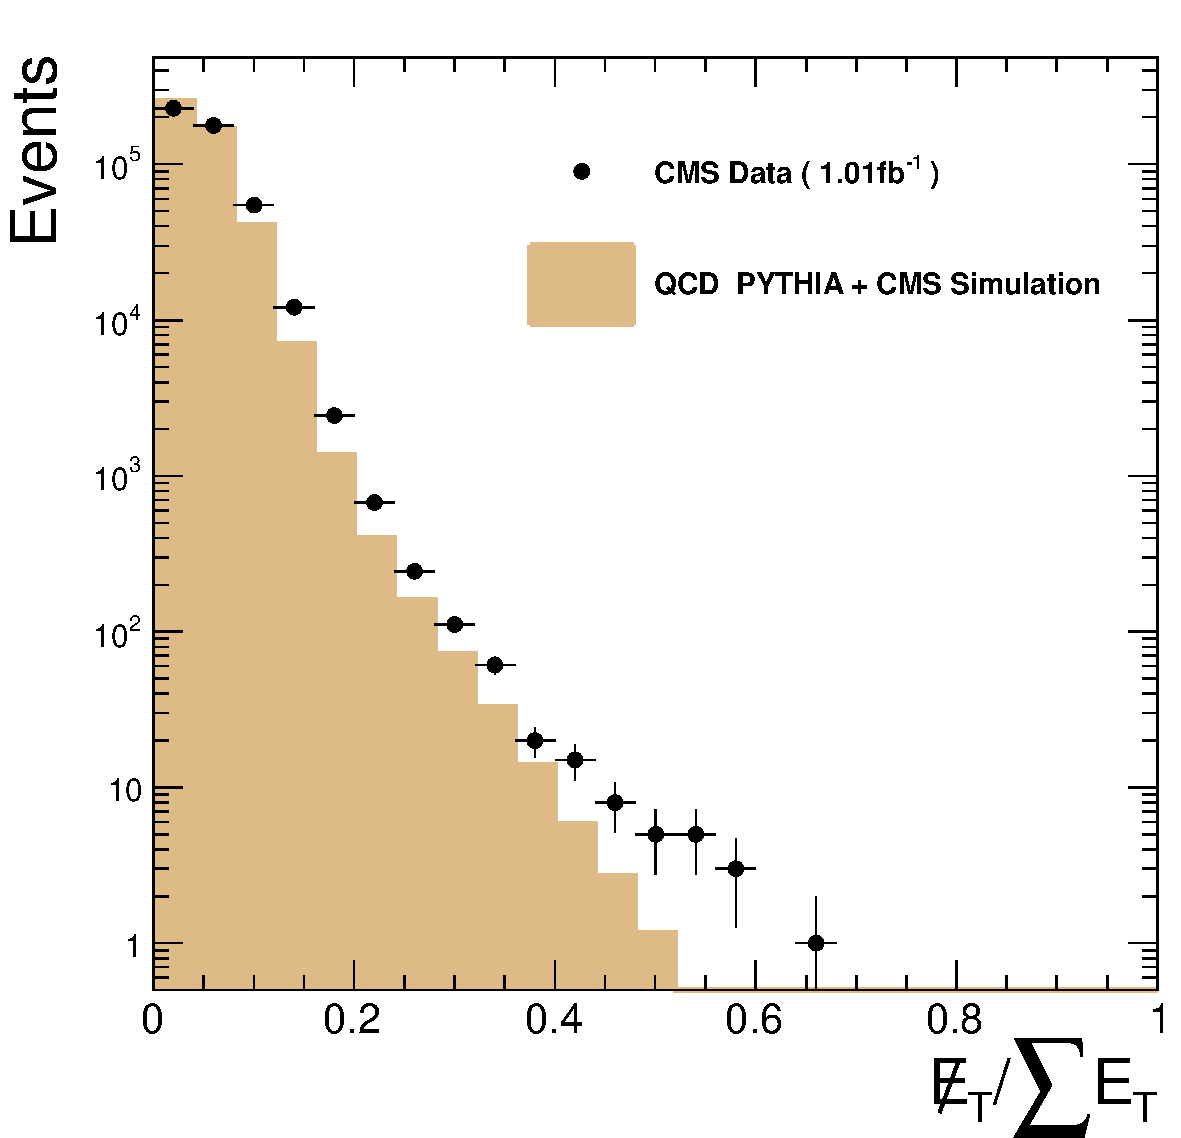
\includegraphics[width=0.45\textwidth]{Figures/c_MET_over_sumEt_log.pdf}
   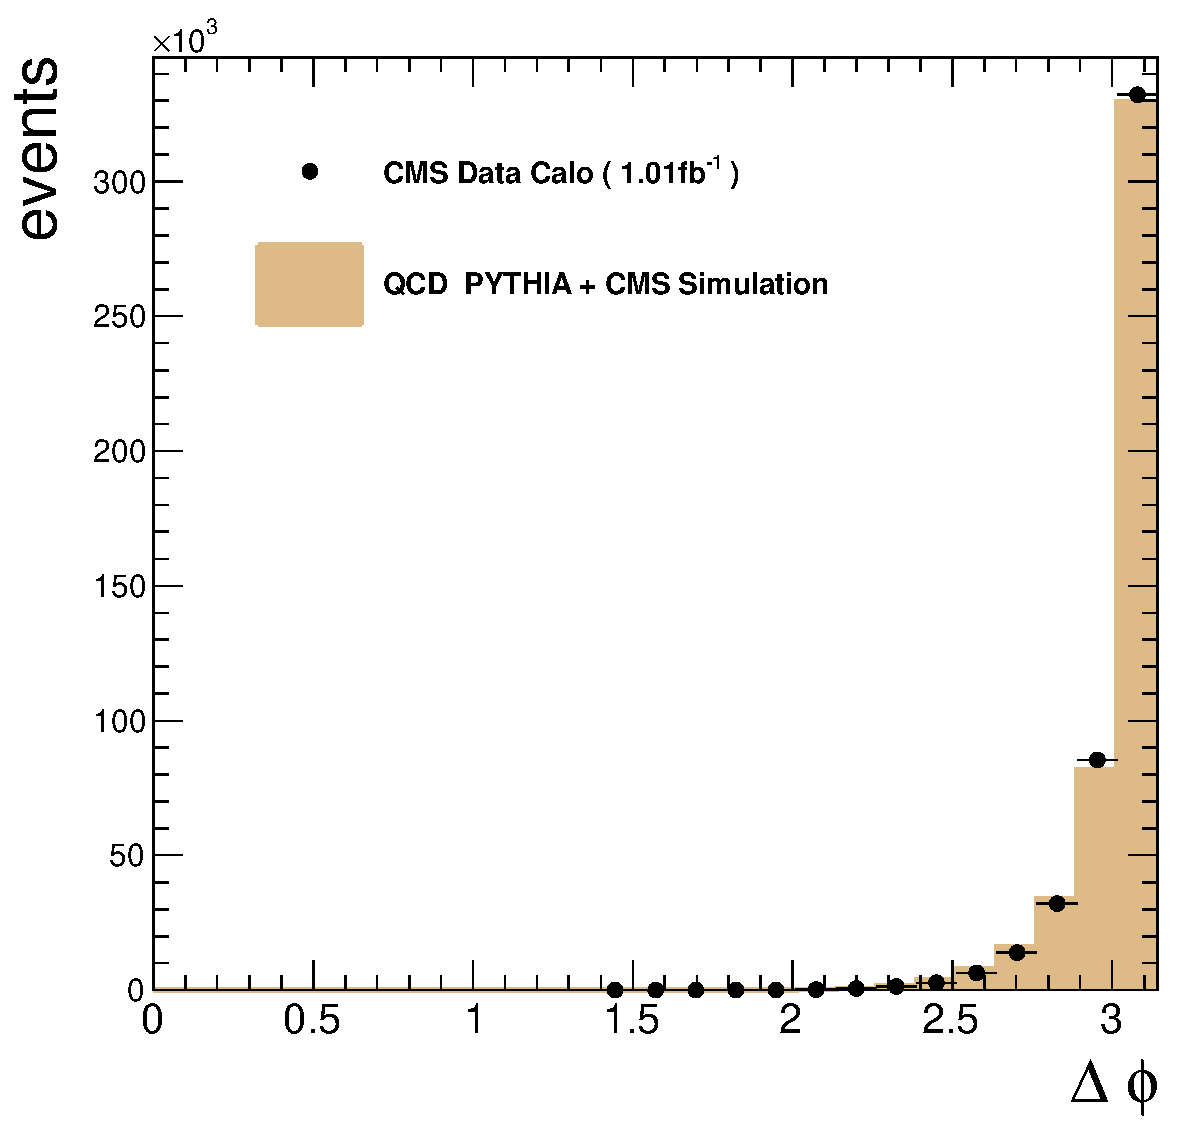
\includegraphics[width=0.45\textwidth]{Figures/c_DPhi.pdf}
   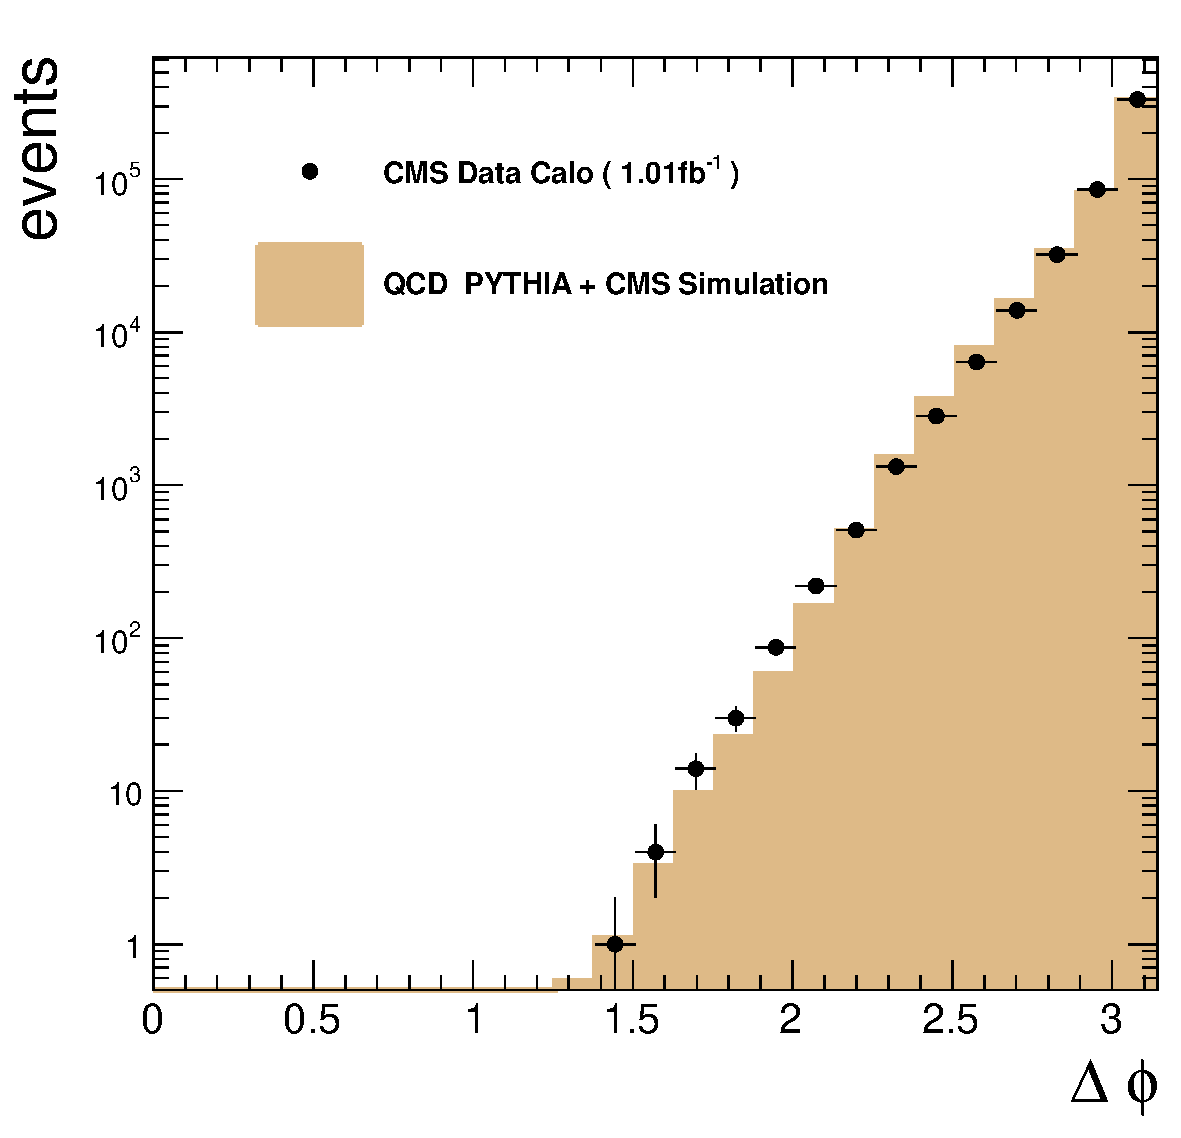
\includegraphics[width=0.45\textwidth]{Figures/c_DPhi_log.pdf}

   \caption{ Event balance distributions for calo jet.  Missing
    calorimeter $E_T$ divided by total calorimeter $E_T$ 
    (upper left) and the same in log scale (upper right).
    The $\phi$ difference of the two leading jets (lower left) 
    and the same in log scale (lower right).}
    \label{basic_event_calo}
  \end{center}
\end{figure}

\begin{figure}[!ht]
  \begin{center}
   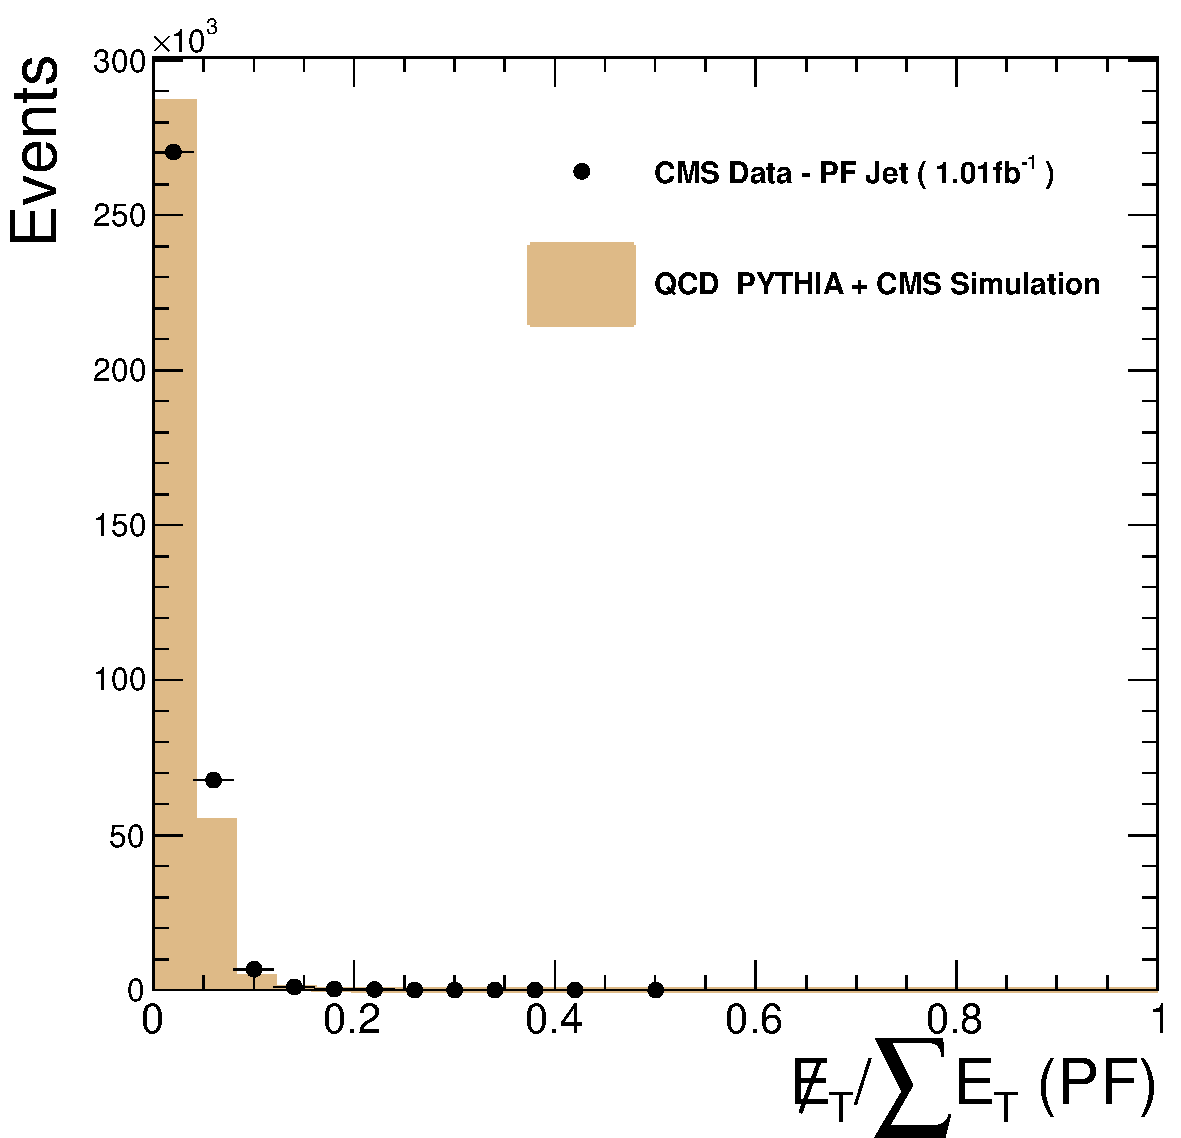
\includegraphics[width=0.45\textwidth]{Figures/c_MET_over_sumEt_pf.pdf}
   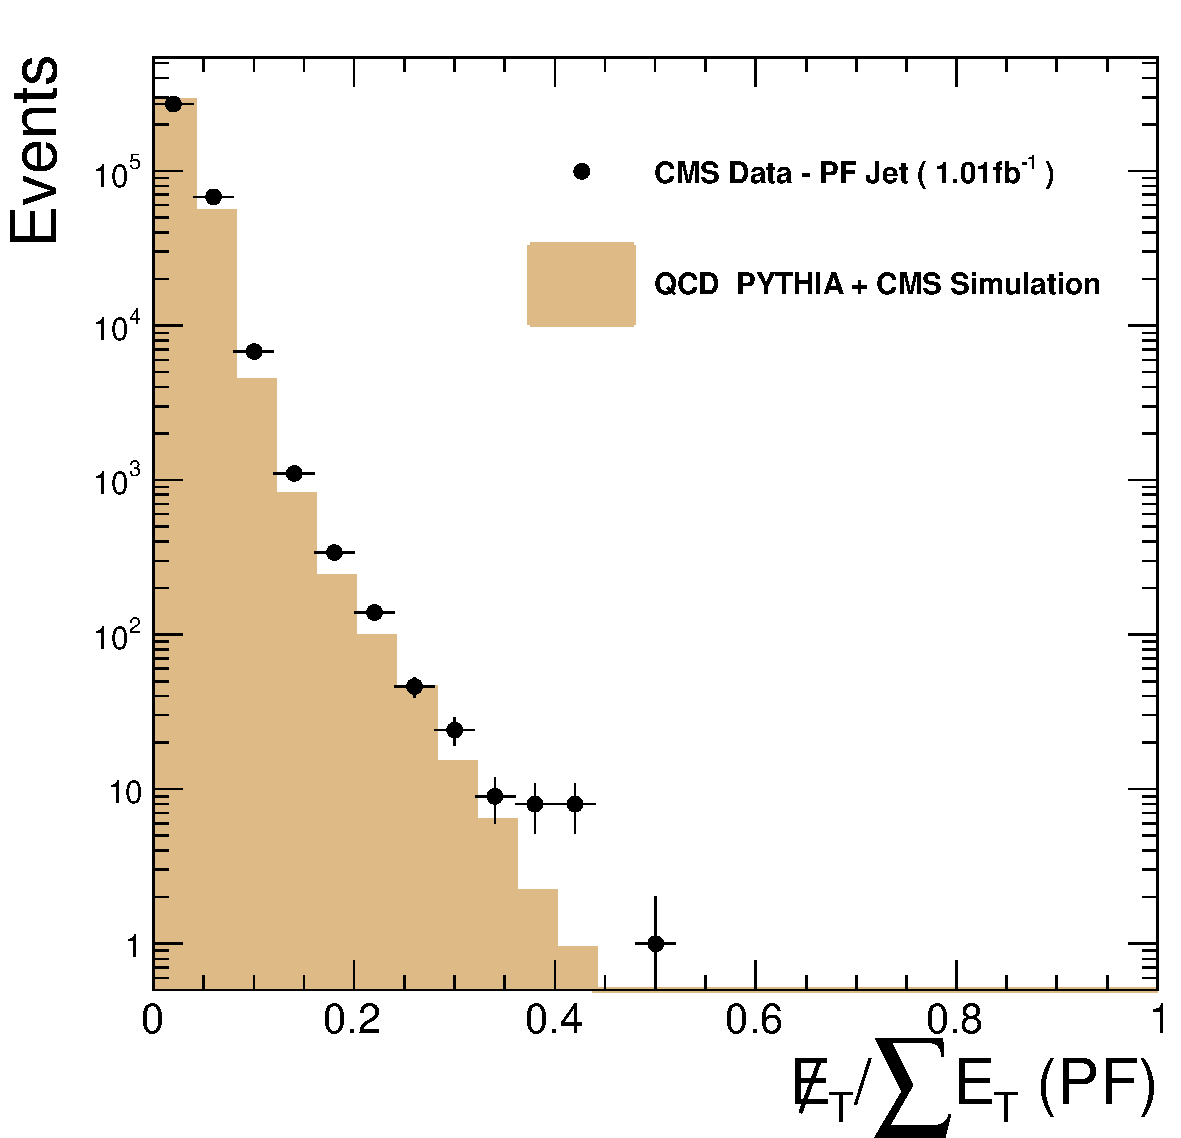
\includegraphics[width=0.45\textwidth]{Figures/c_MET_over_sumEt_pf_log.pdf}
   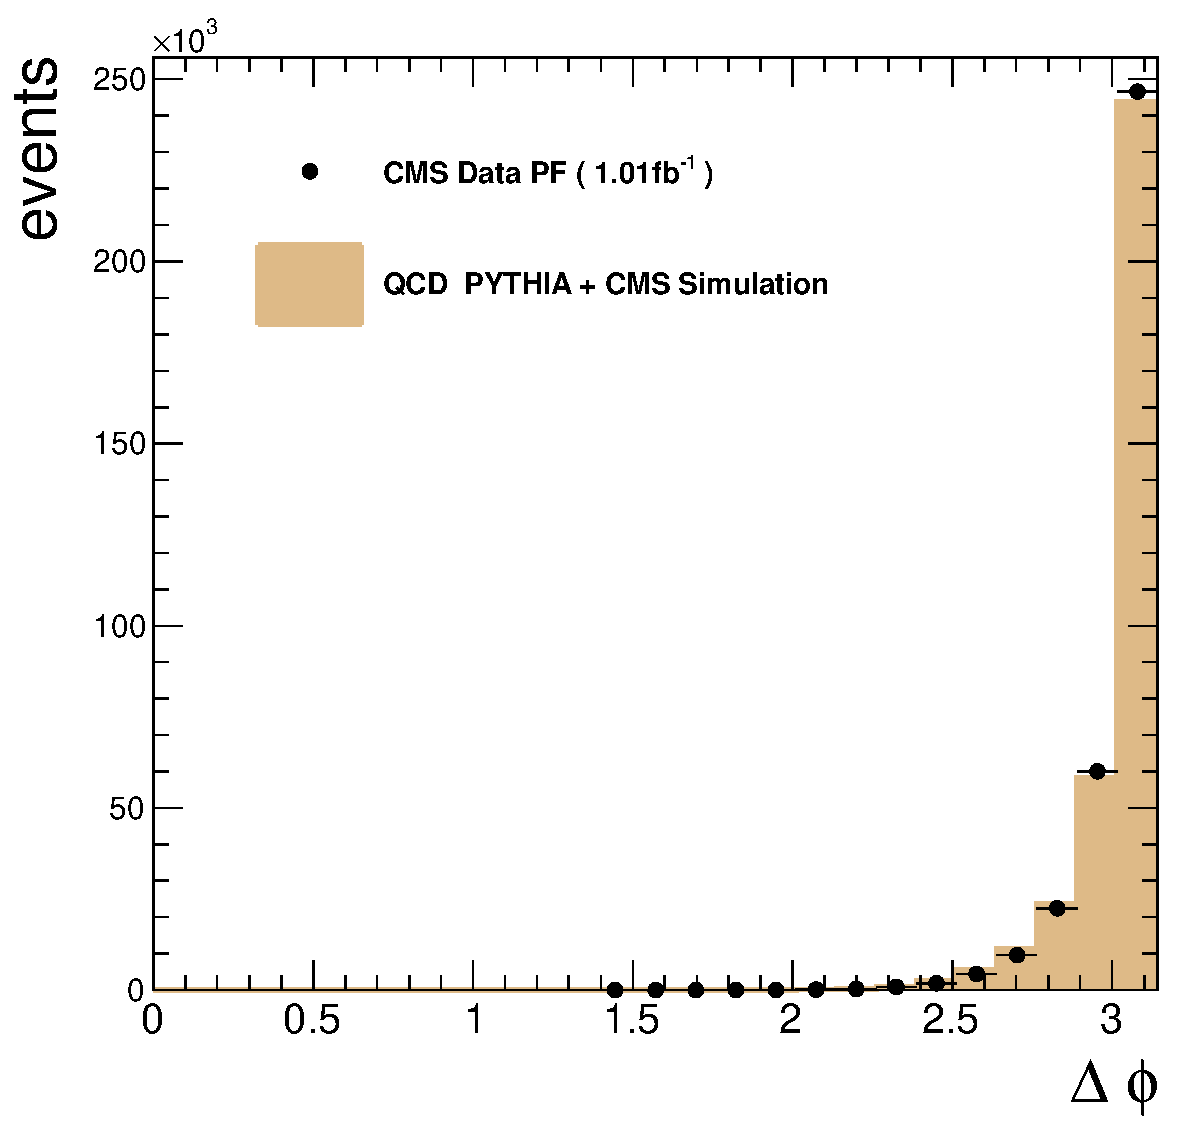
\includegraphics[width=0.45\textwidth]{Figures/c_DPhi_pf.pdf}
   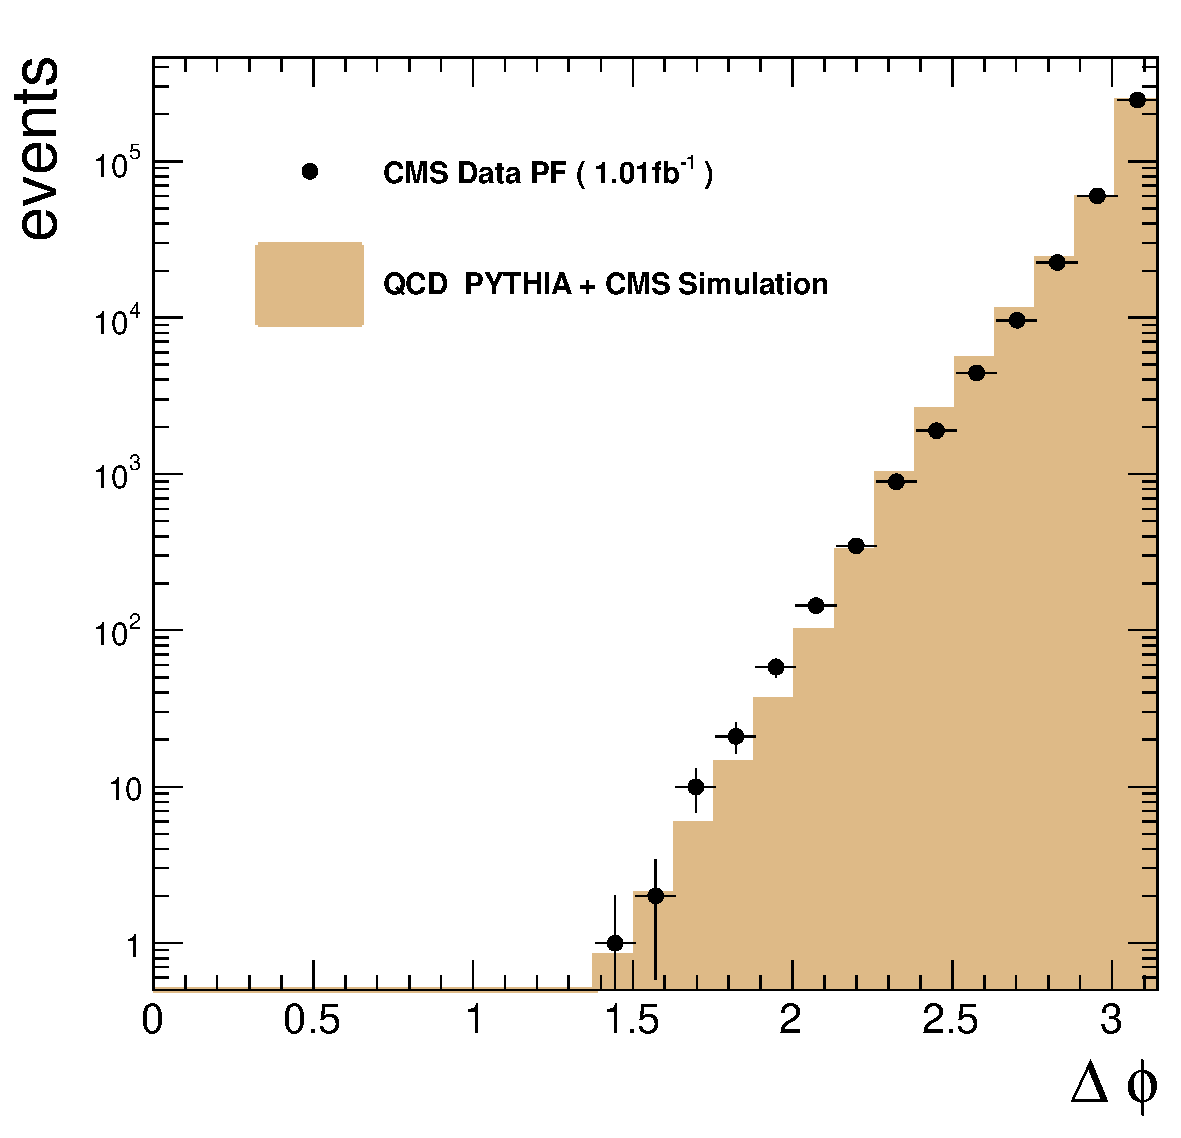
\includegraphics[width=0.45\textwidth]{Figures/c_DPhi_pf_log.pdf}

   \caption{ Event balance distributions for PF Jets.  Missing
    calorimeter $E_T$ divided by total calorimeter $E_T$ 
    (upper left) and the same in log scale (upper right).
    The $\phi$ difference of the two leading jets (lower left) 
    and the same in log scale (lower right).}
    \label{basic_event_pf}
  \end{center}
\end{figure}

\begin{figure}[!ht]
  \begin{center}
   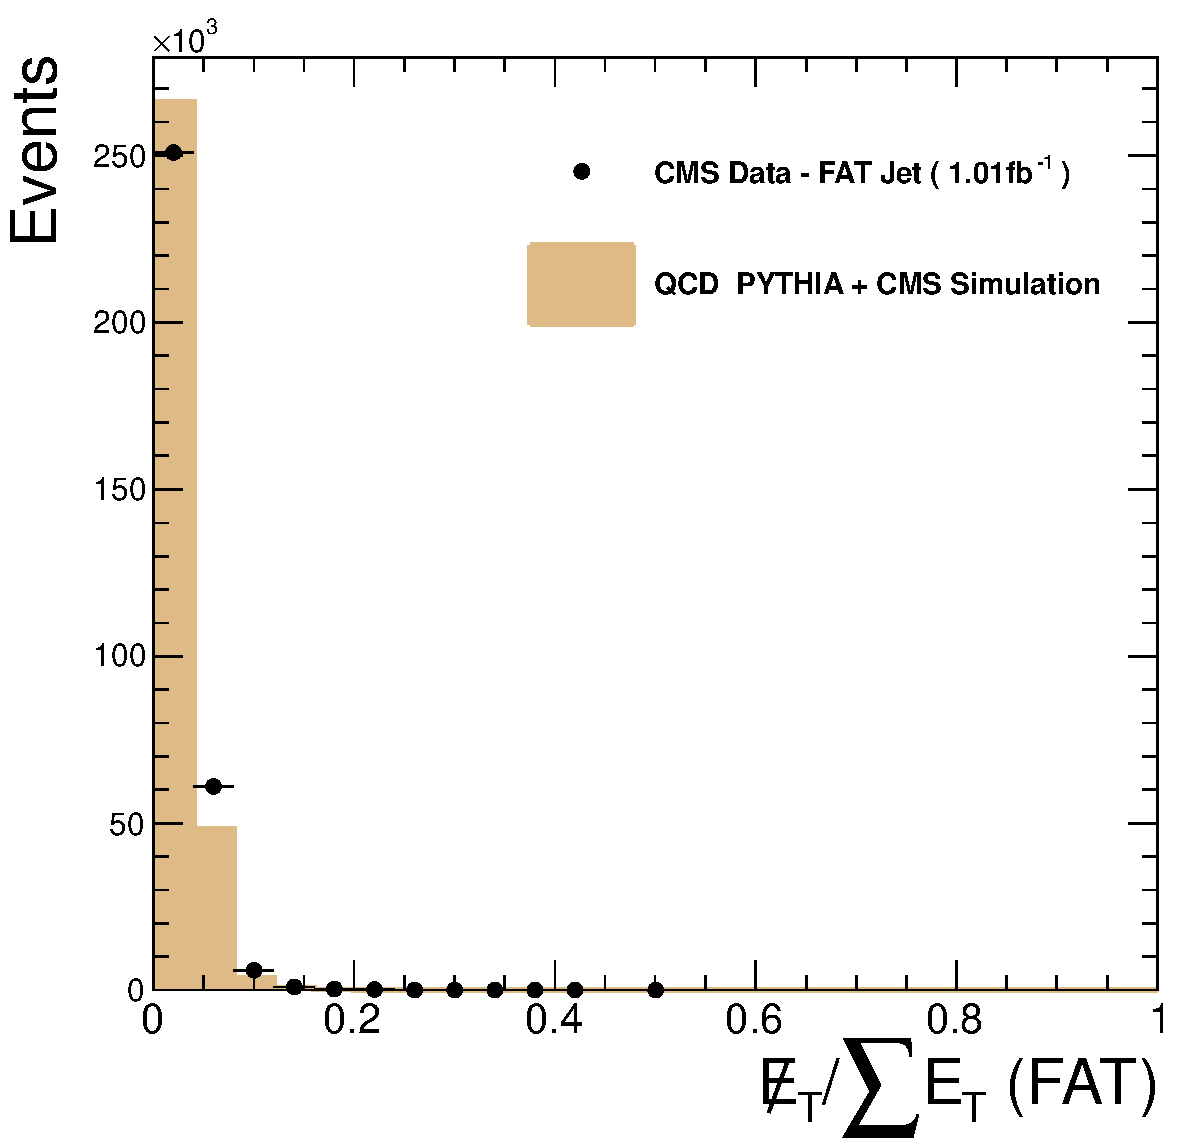
\includegraphics[width=0.45\textwidth]{Figures/c_MET_over_sumEt_fat.pdf}
   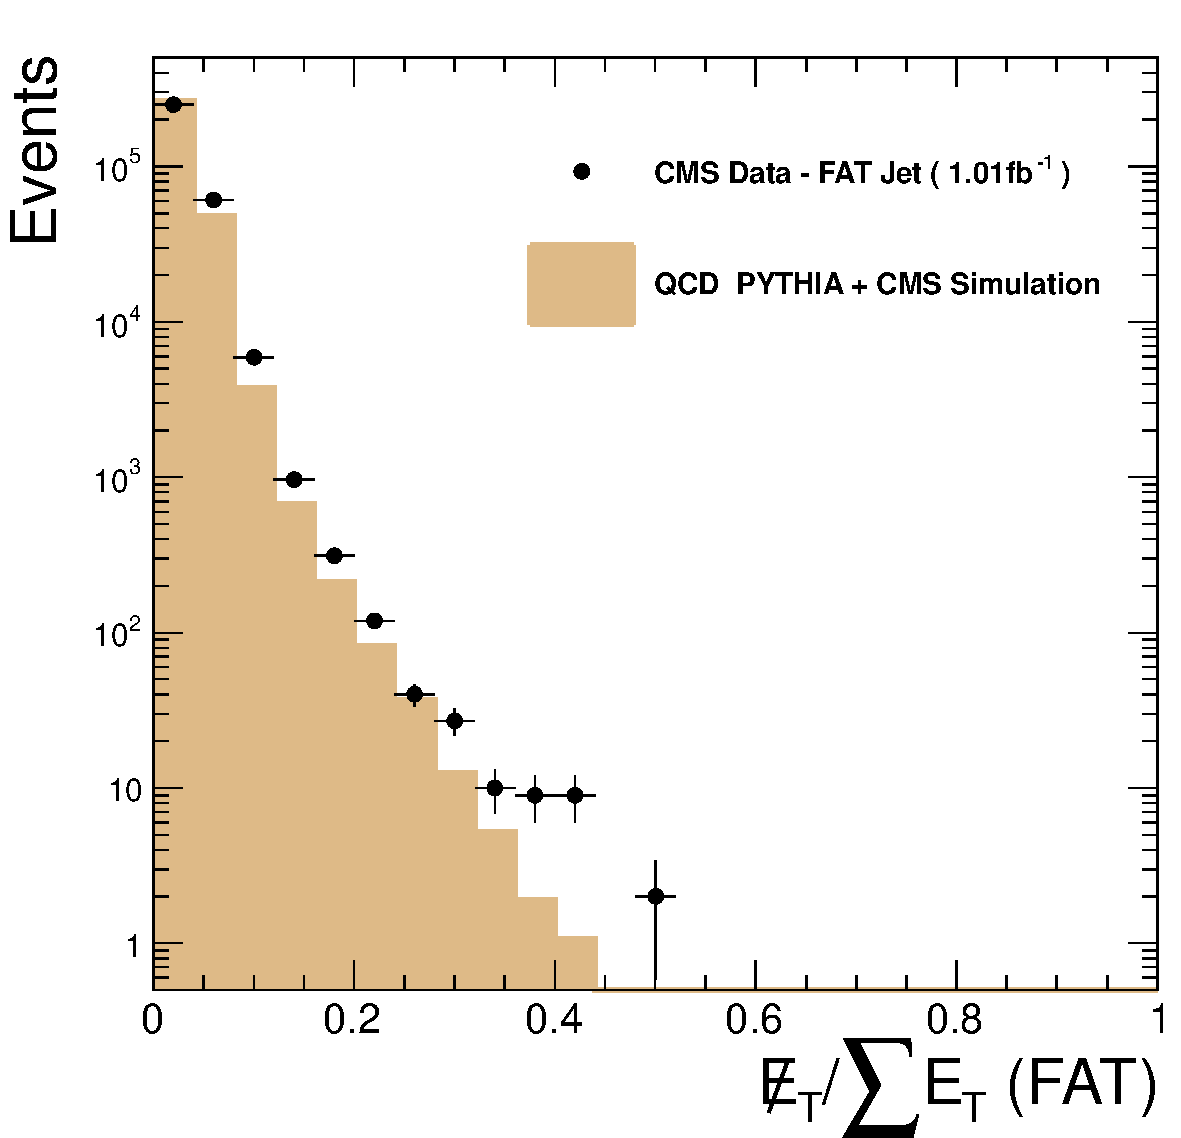
\includegraphics[width=0.45\textwidth]{Figures/c_MET_over_sumEt_fat_log.pdf}
   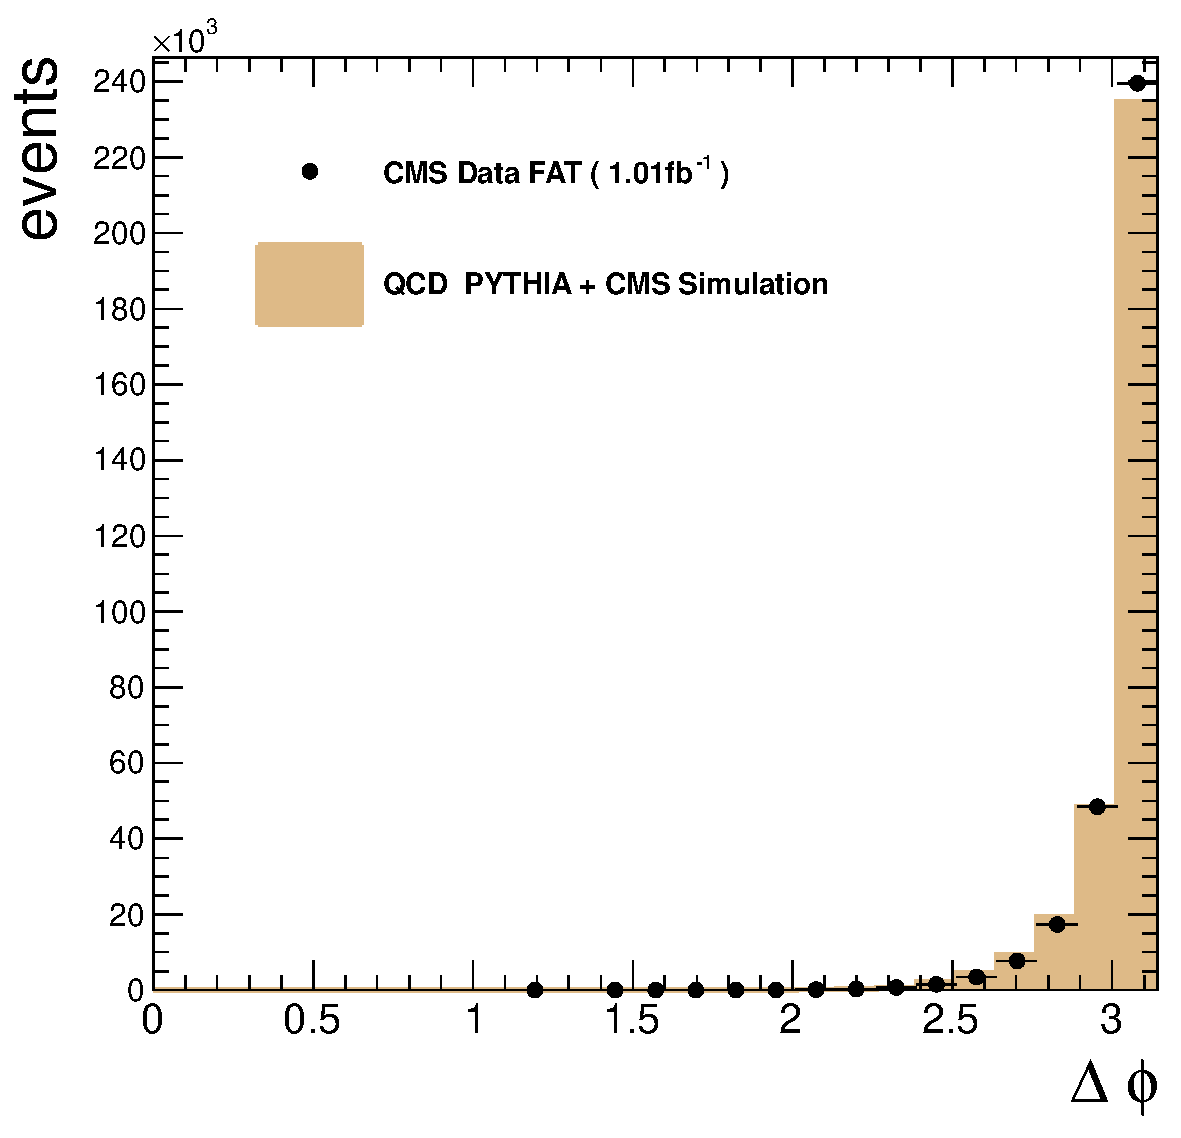
\includegraphics[width=0.45\textwidth]{Figures/c_DPhi_fat.pdf}
   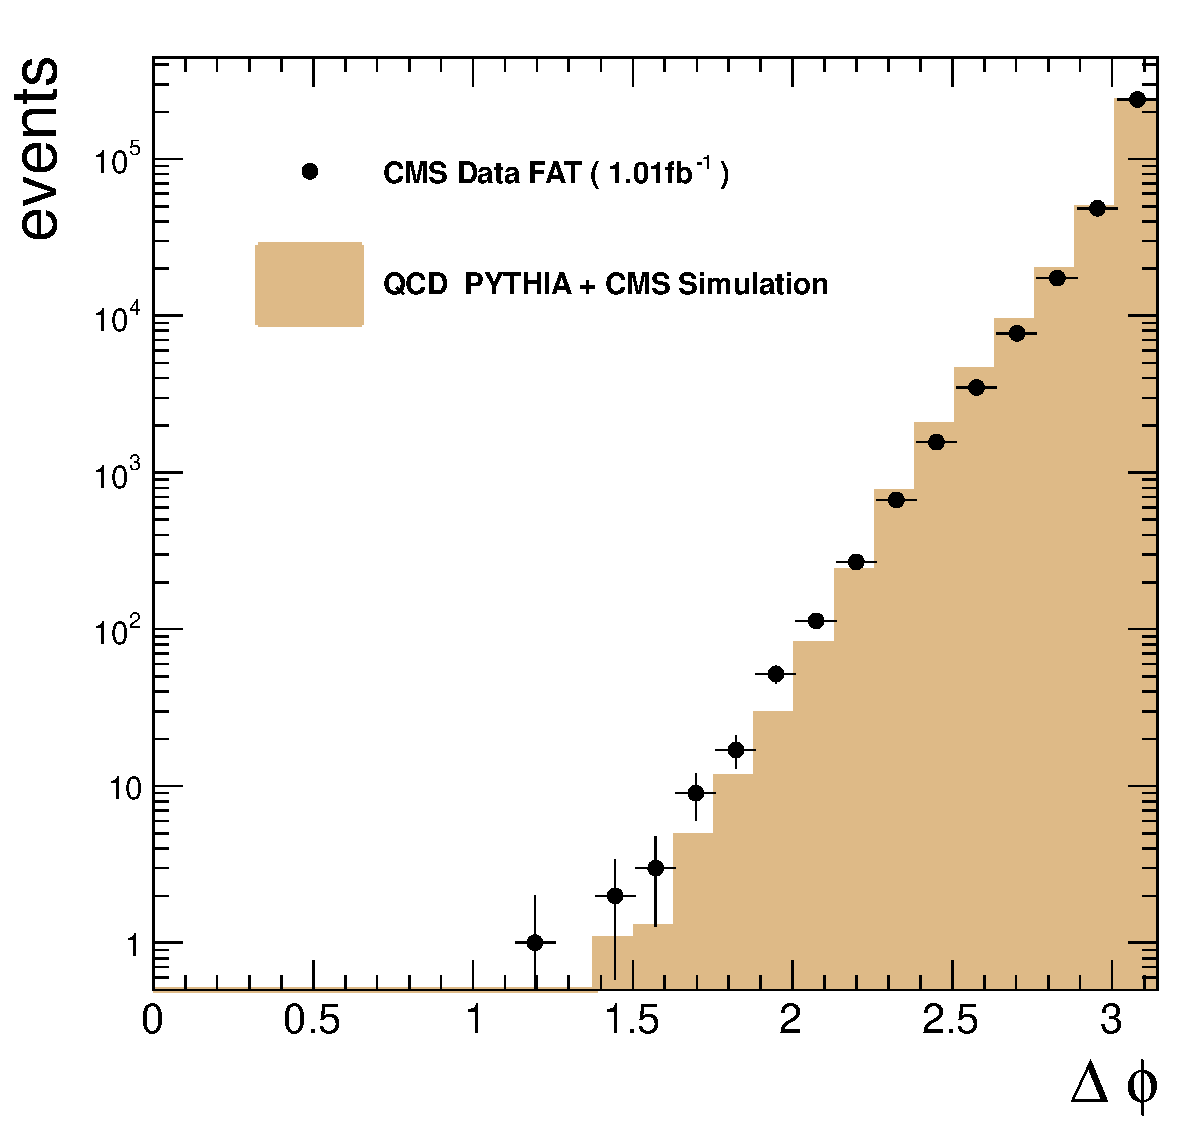
\includegraphics[width=0.45\textwidth]{Figures/c_DPhi_fat_log.pdf}

   \caption{ Event balance distributions for Wide Jets.  Missing
    calorimeter $E_T$ divided by total calorimeter $E_T$ 
    (upper left) and the same in log scale (upper right).
    The $\phi$ difference of the two leading jets (lower left) 
    and the same in log scale (lower right).}
    \label{basic_event_pf}
  \end{center}
\end{figure}

\begin{figure}[!ht]
  \begin{center}
    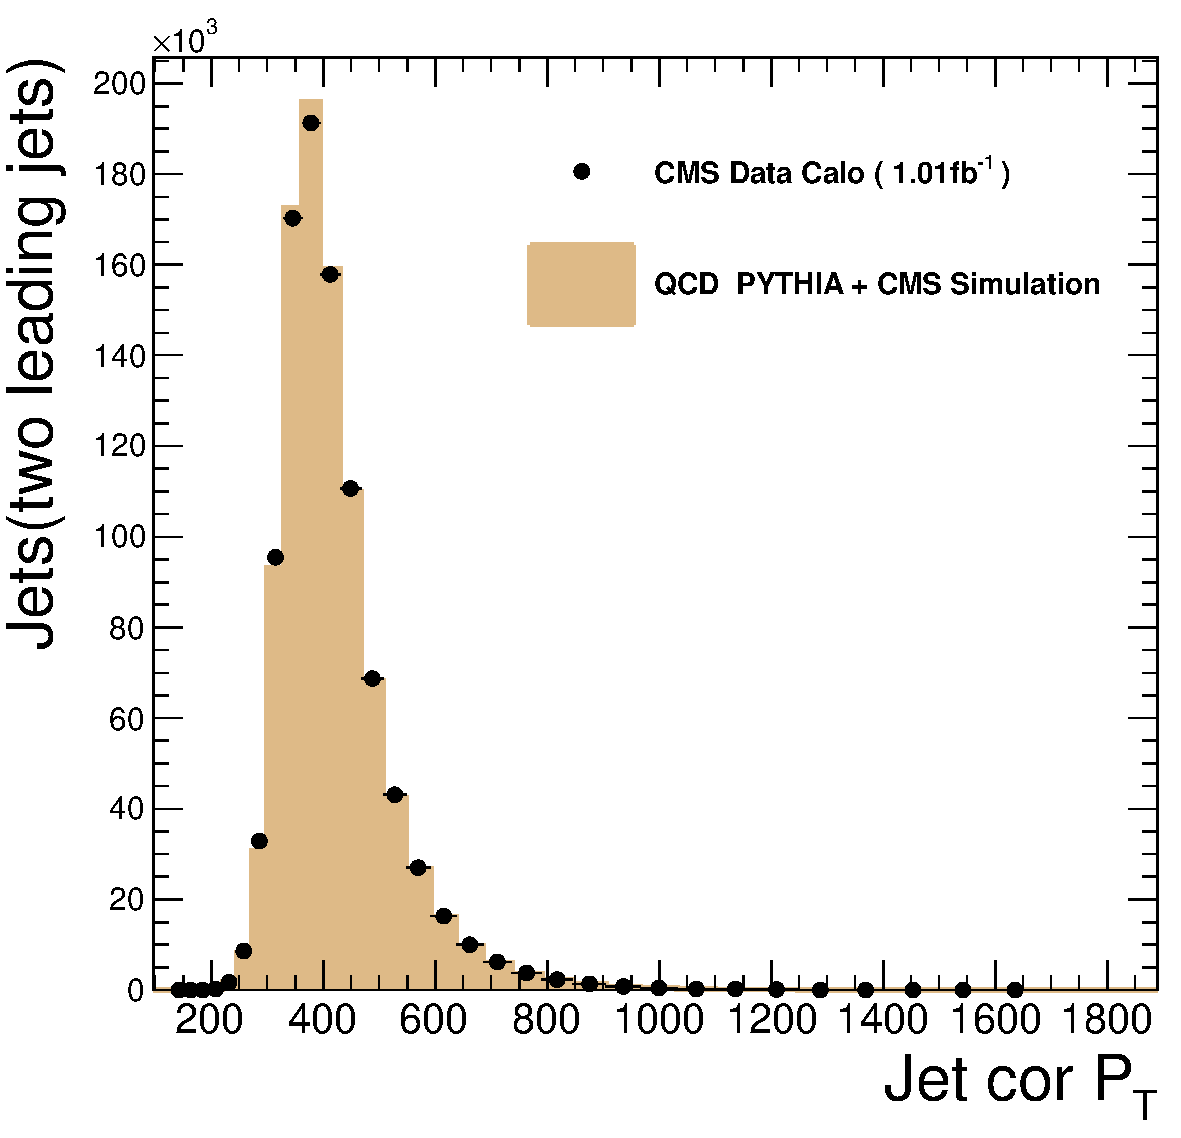
\includegraphics[width=0.45\textwidth]{Figures/c_corPt.pdf}
    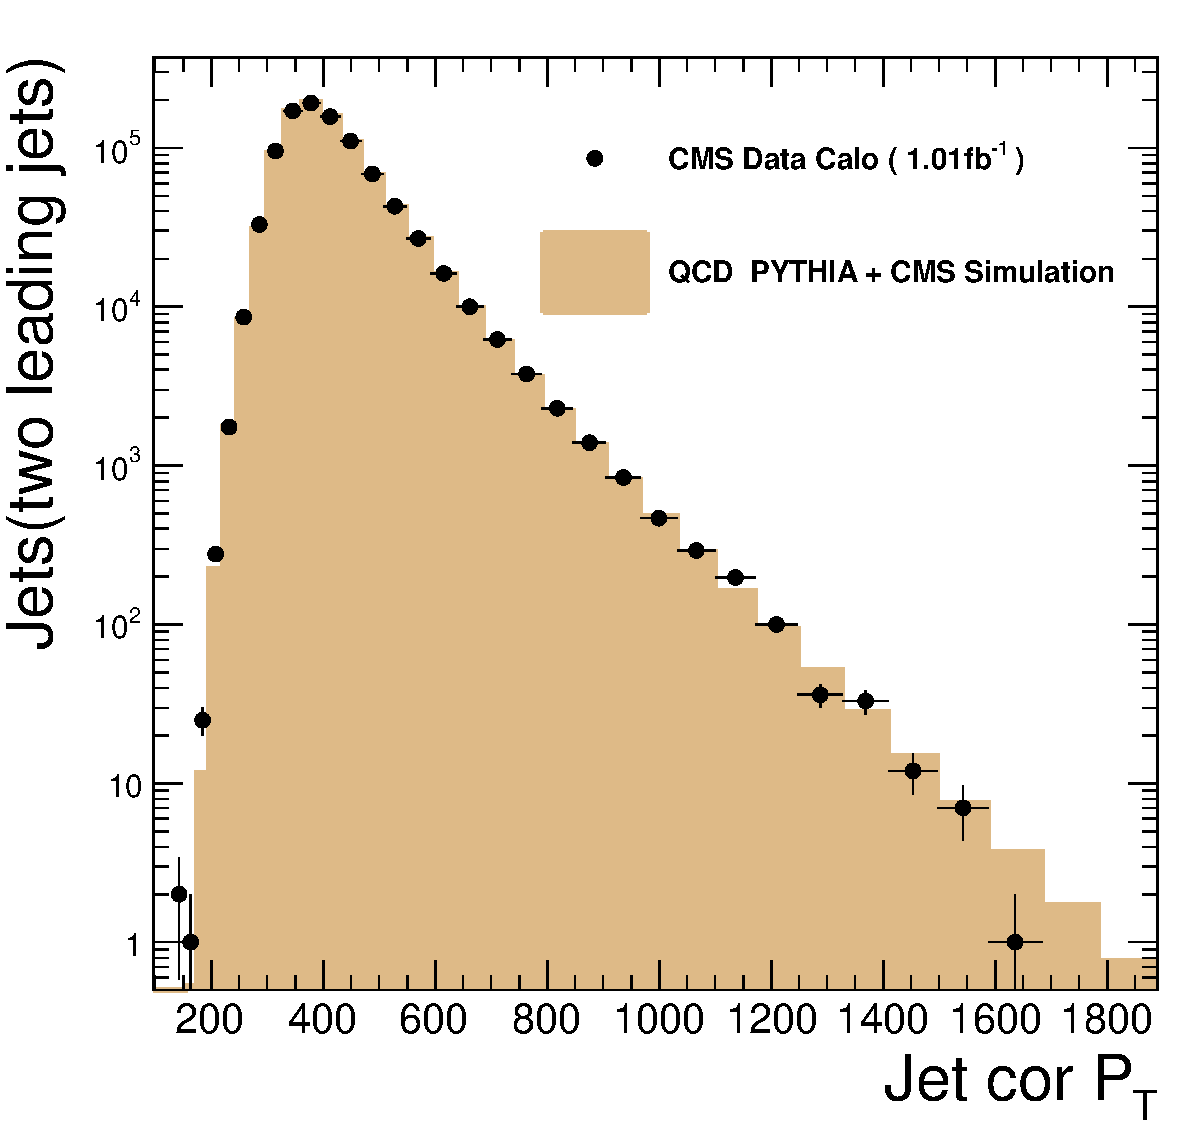
\includegraphics[width=0.45\textwidth]{Figures/c_corPt_log.pdf}
    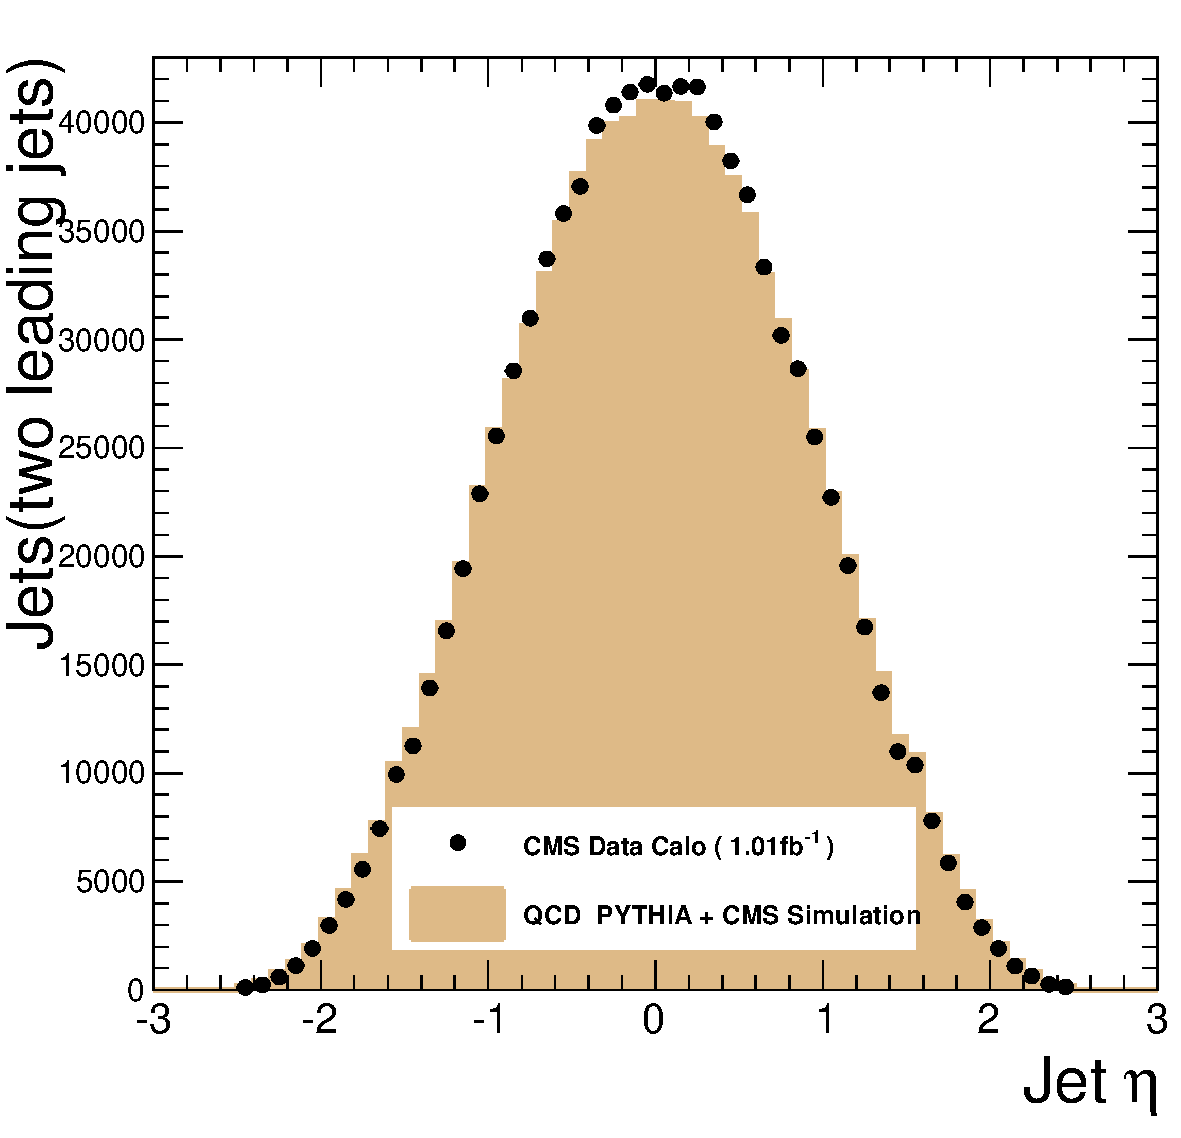
\includegraphics[width=0.45\textwidth]{Figures/c_Eta.pdf}
    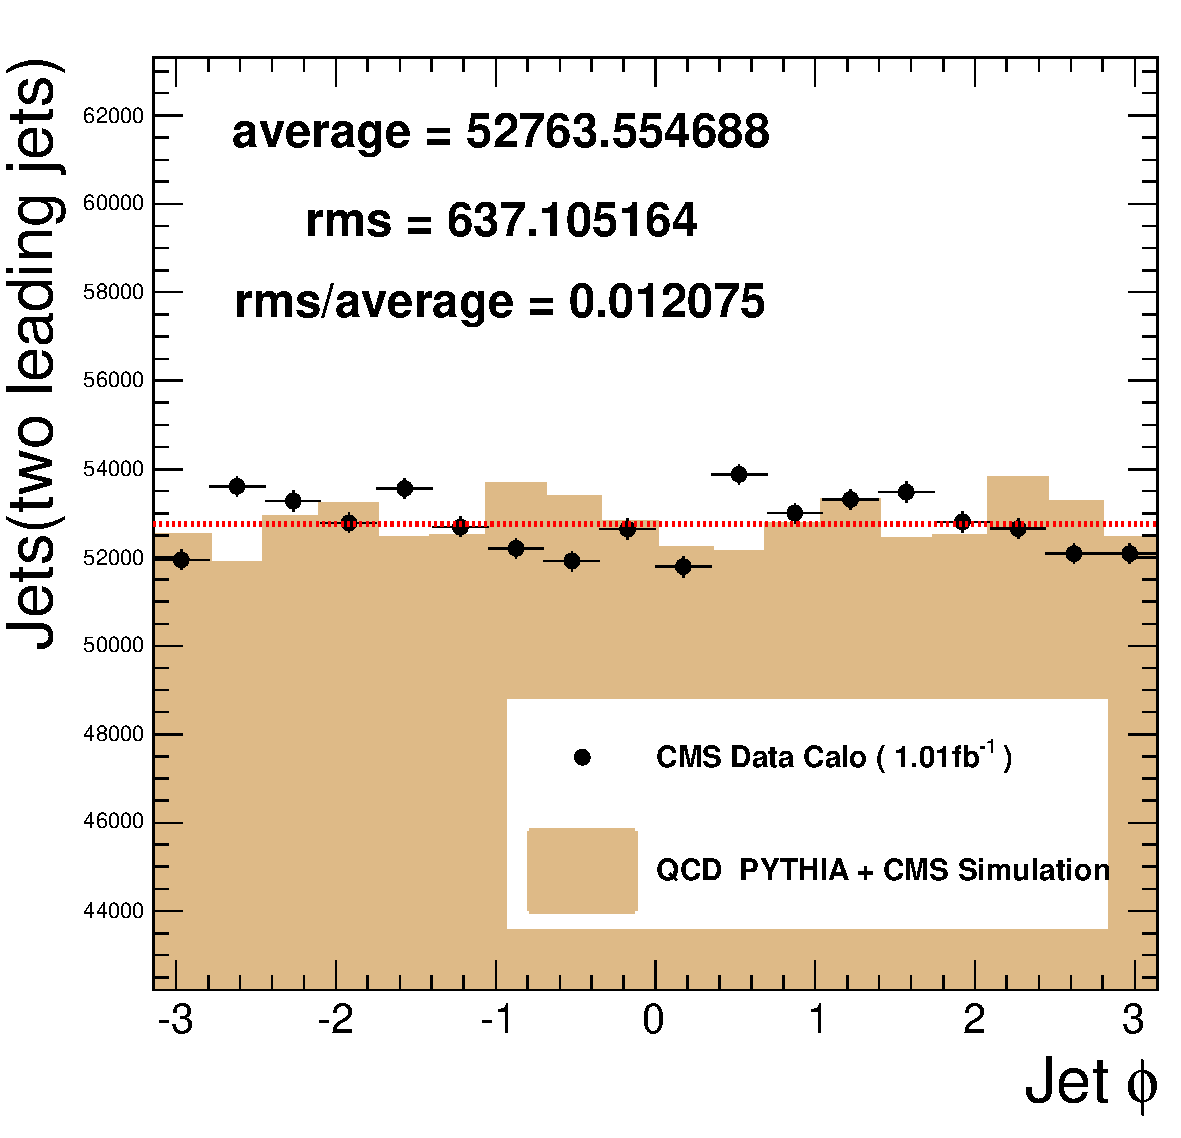
\includegraphics[width=0.45\textwidth]{Figures/c_Phi.pdf}
    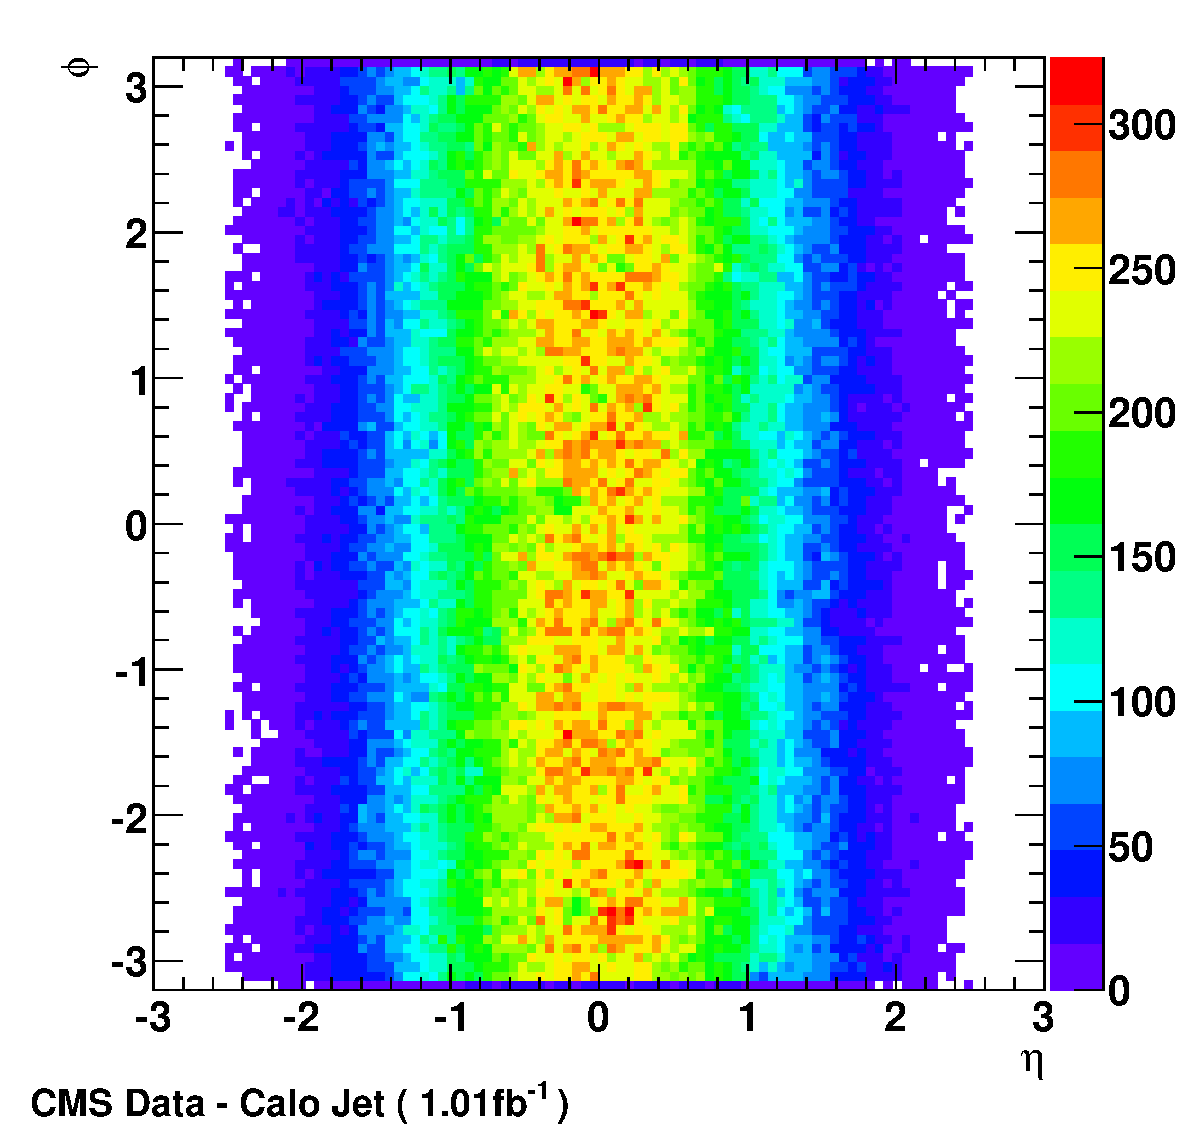
\includegraphics[width=0.45\textwidth]{Figures/c_Eta_Phi_Scatter.pdf}
    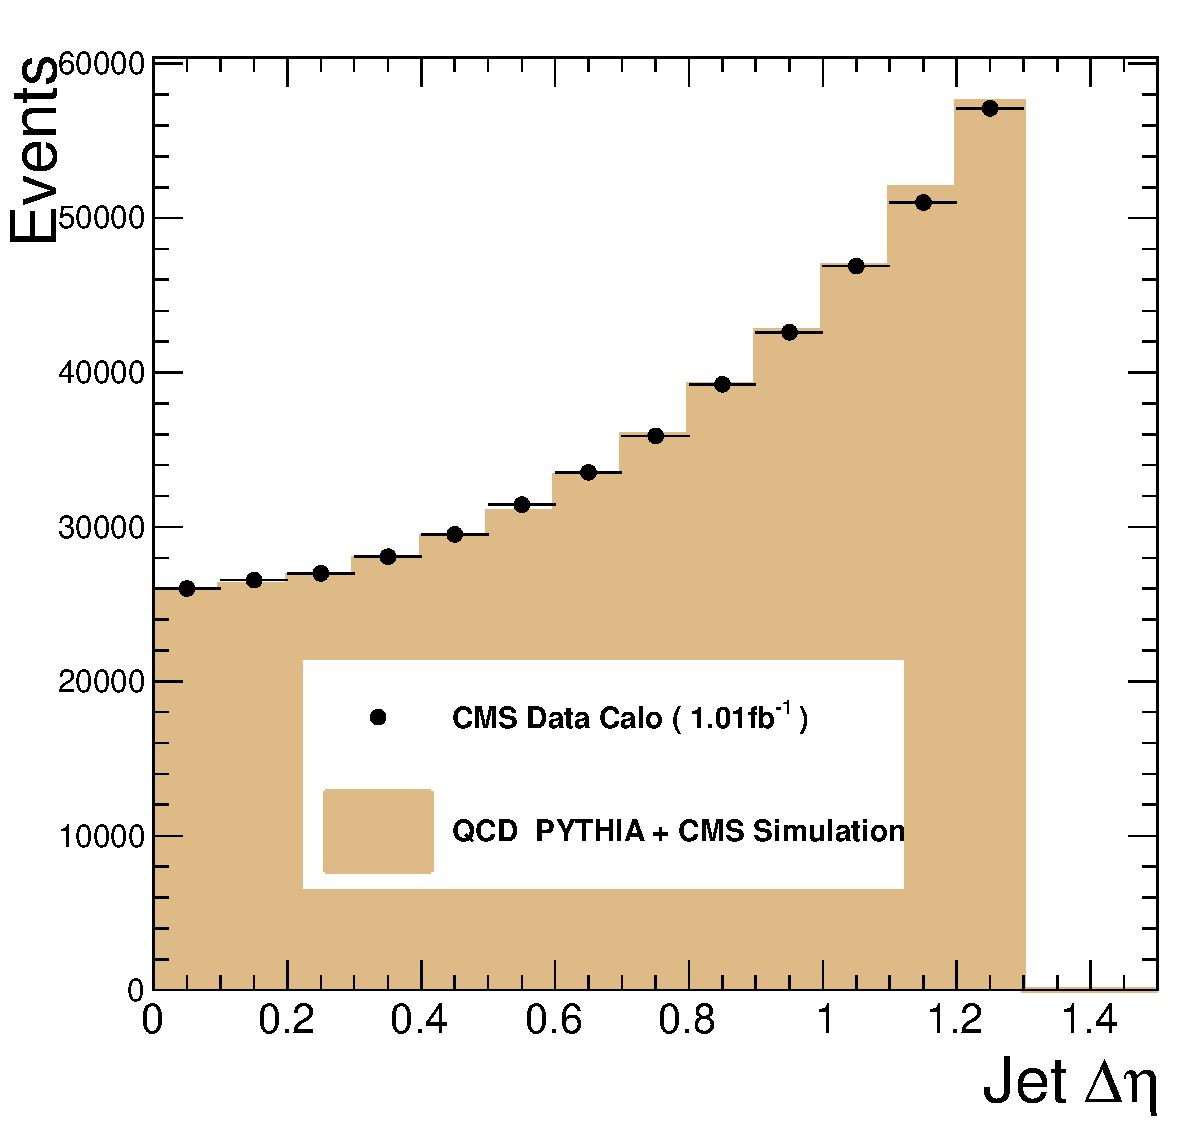
\includegraphics[width=0.45\textwidth]{Figures/c_DEta.pdf}

    \caption{ Jet kinematics distributions for calo jets.  The corrected $P_T$ of
      the two leading jets (upper left) and the same in log scale
      (upper right). The $\eta$ distribution for the two leading jets
      (middle left). The $\phi$ distribution for the two leading
      jets. (middle right) $\phi$ vs. $\eta$ (lower left) for the two
      leading jets. The $\Delta\eta$ distribution (lower right) }
    \label{jet_kinematics_calo}
  \end{center}
\end{figure}

\begin{figure}[!ht]
  \begin{center}
    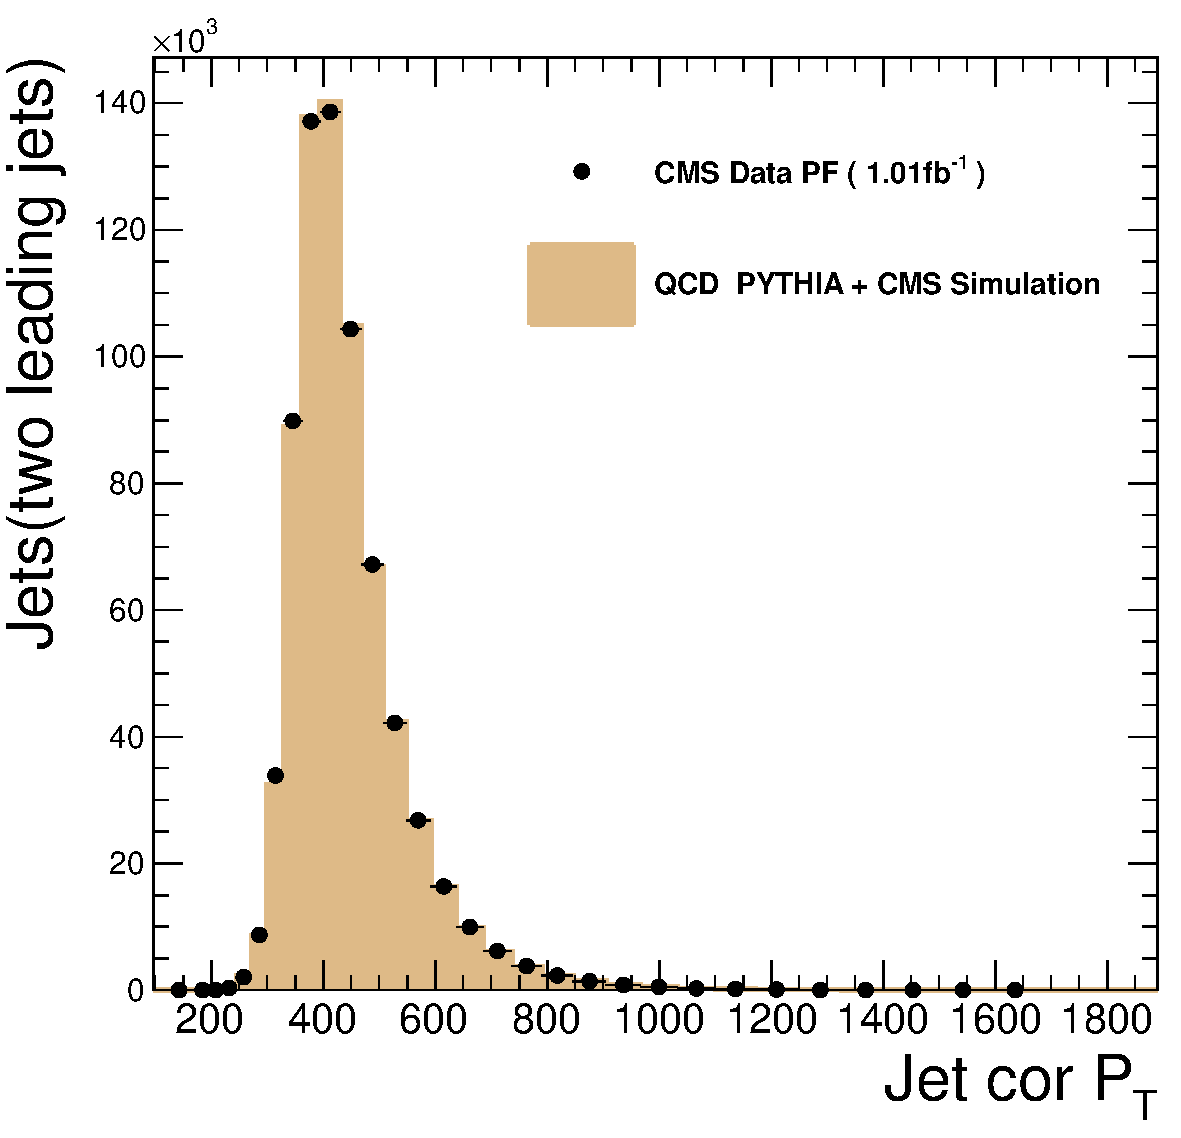
\includegraphics[width=0.45\textwidth]{Figures/c_corPt_pf.pdf}
    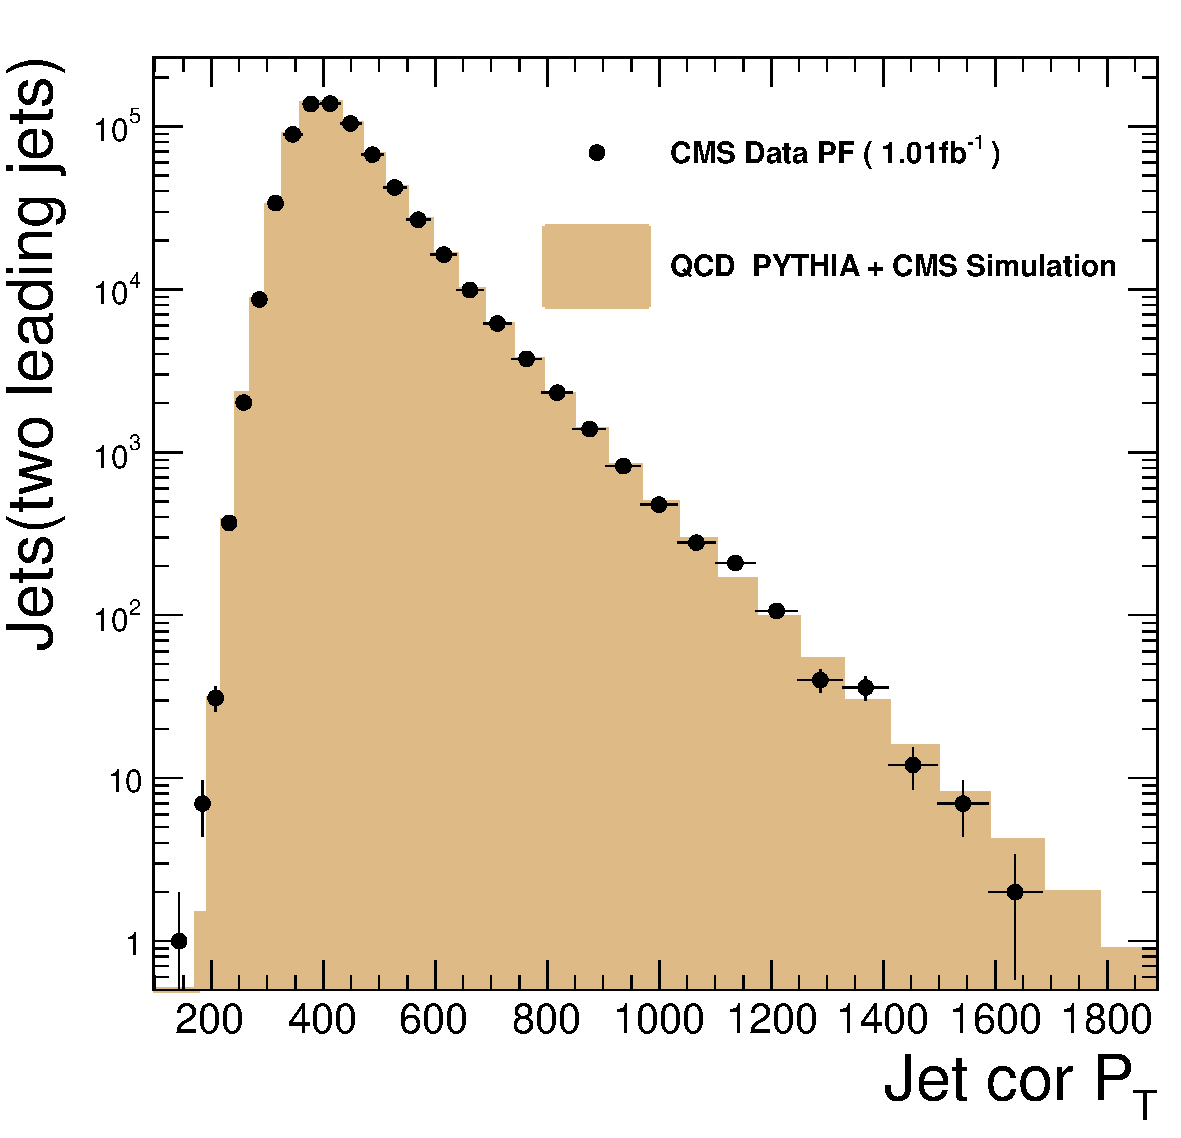
\includegraphics[width=0.45\textwidth]{Figures/c_corPt_pf_log.pdf}
    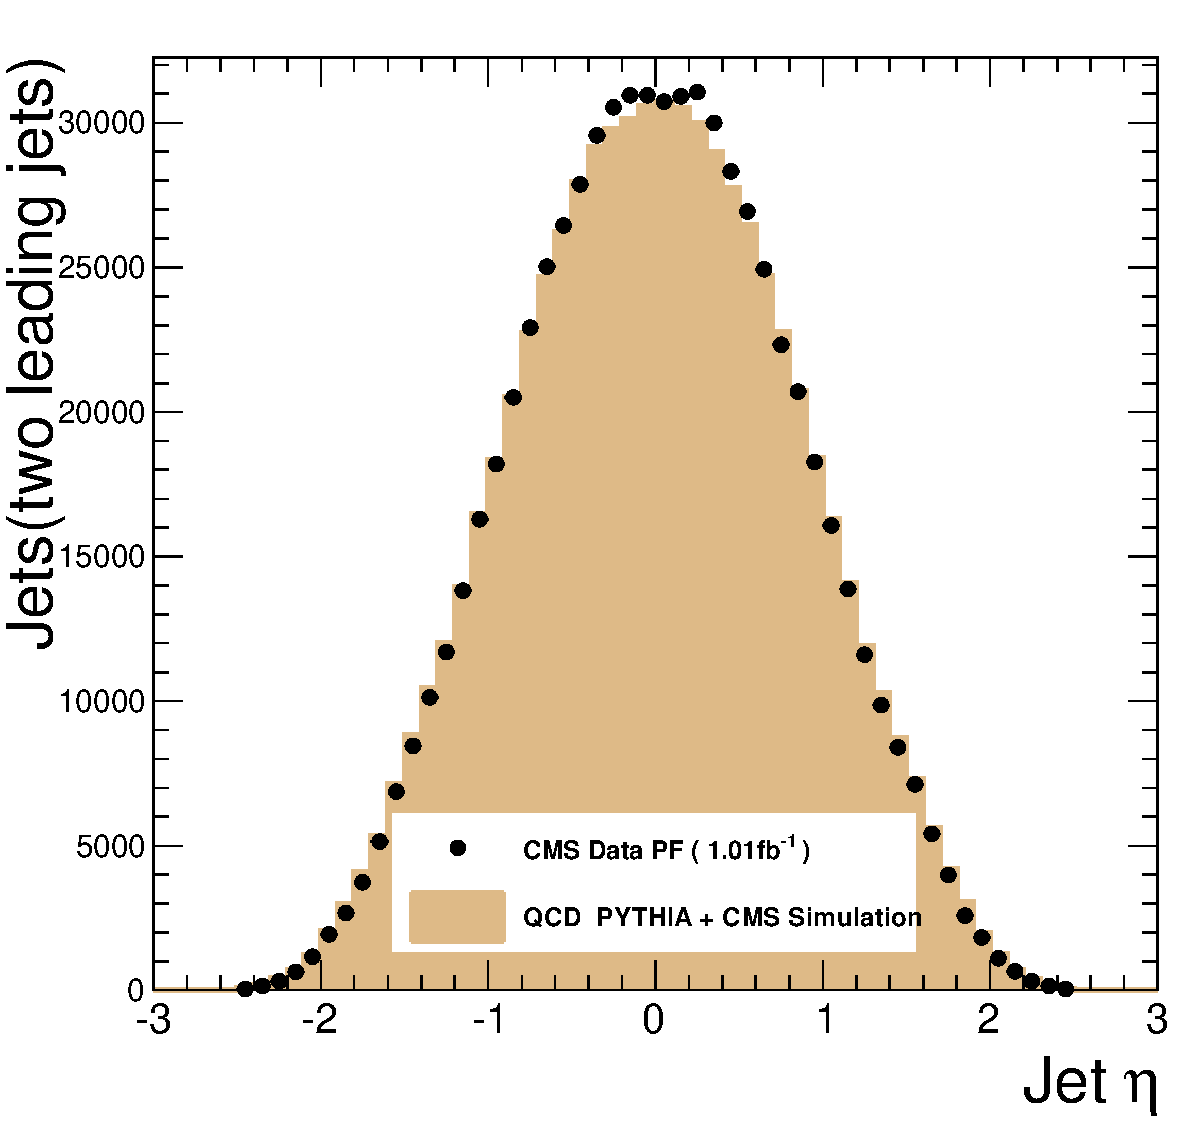
\includegraphics[width=0.45\textwidth]{Figures/c_Eta_pf.pdf}
    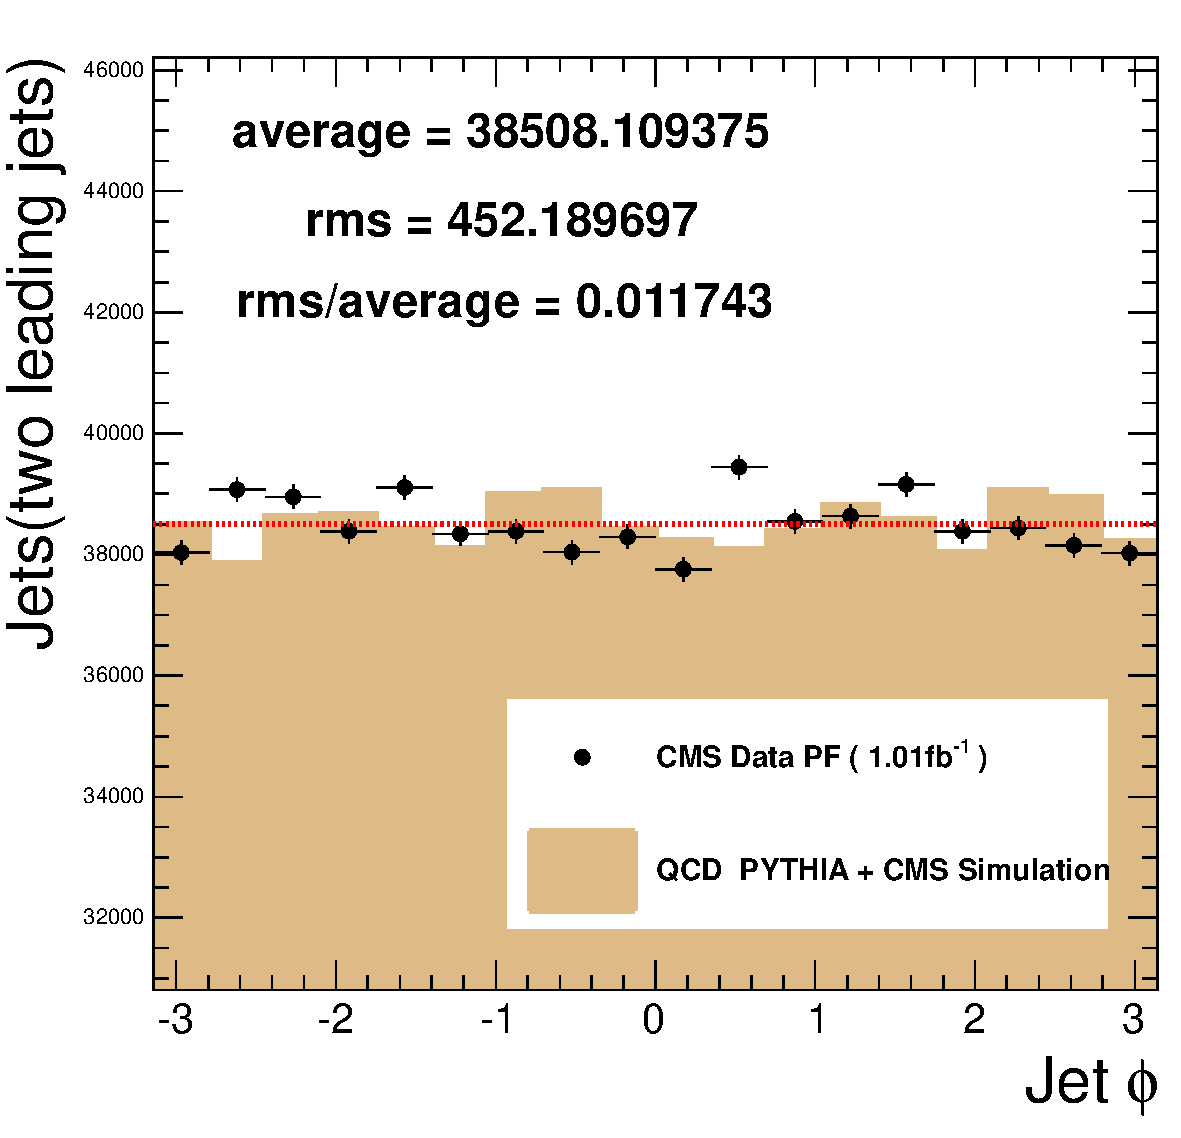
\includegraphics[width=0.45\textwidth]{Figures/c_Phi_pf.pdf}
    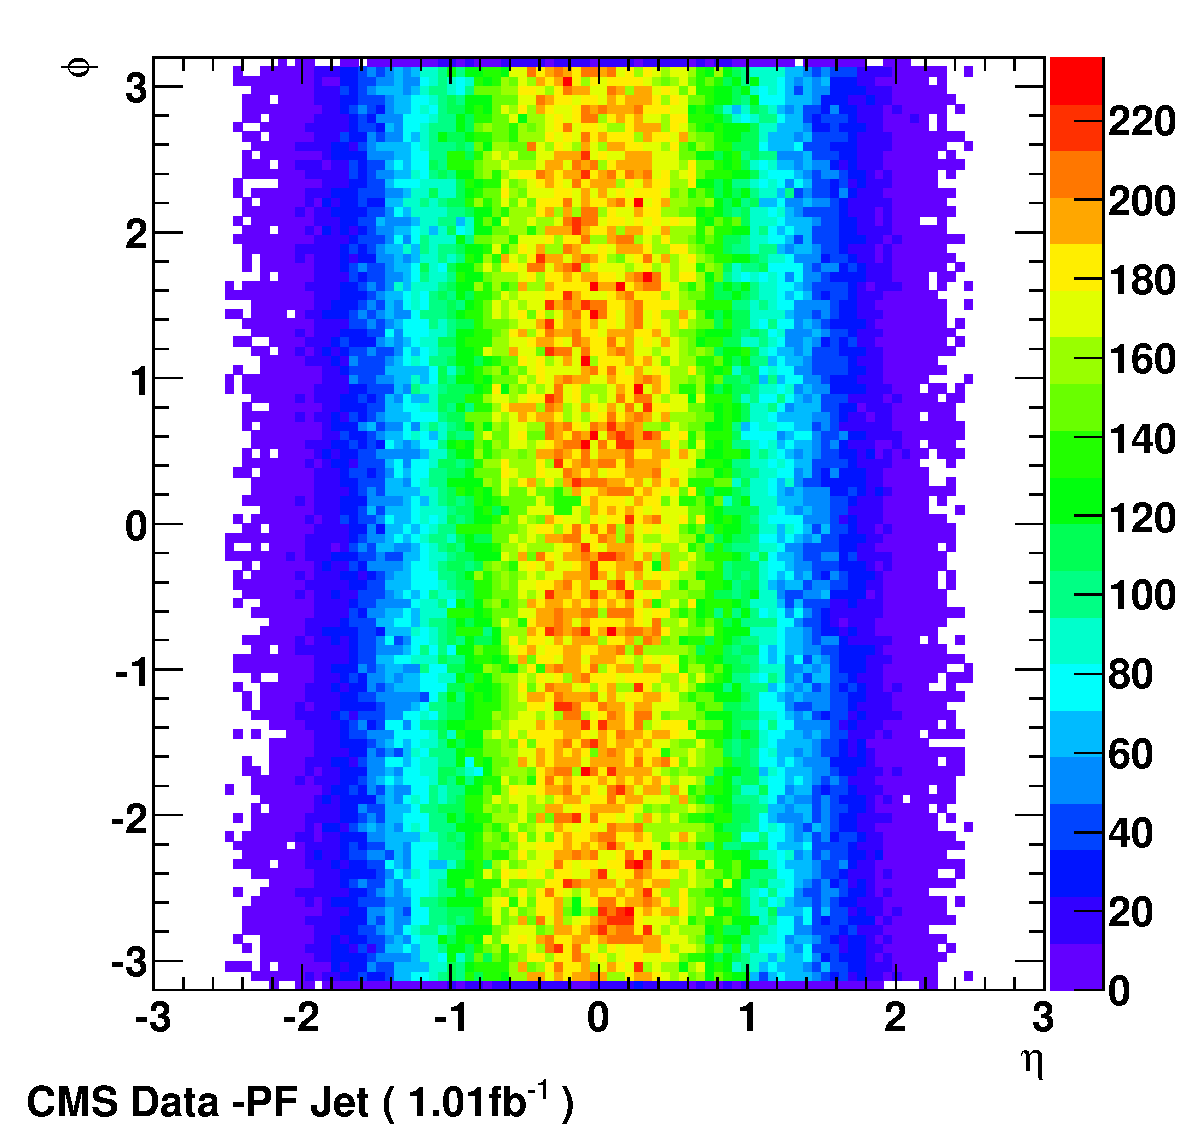
\includegraphics[width=0.45\textwidth]{Figures/c_Eta_Phi_Scatter_pf.pdf}
    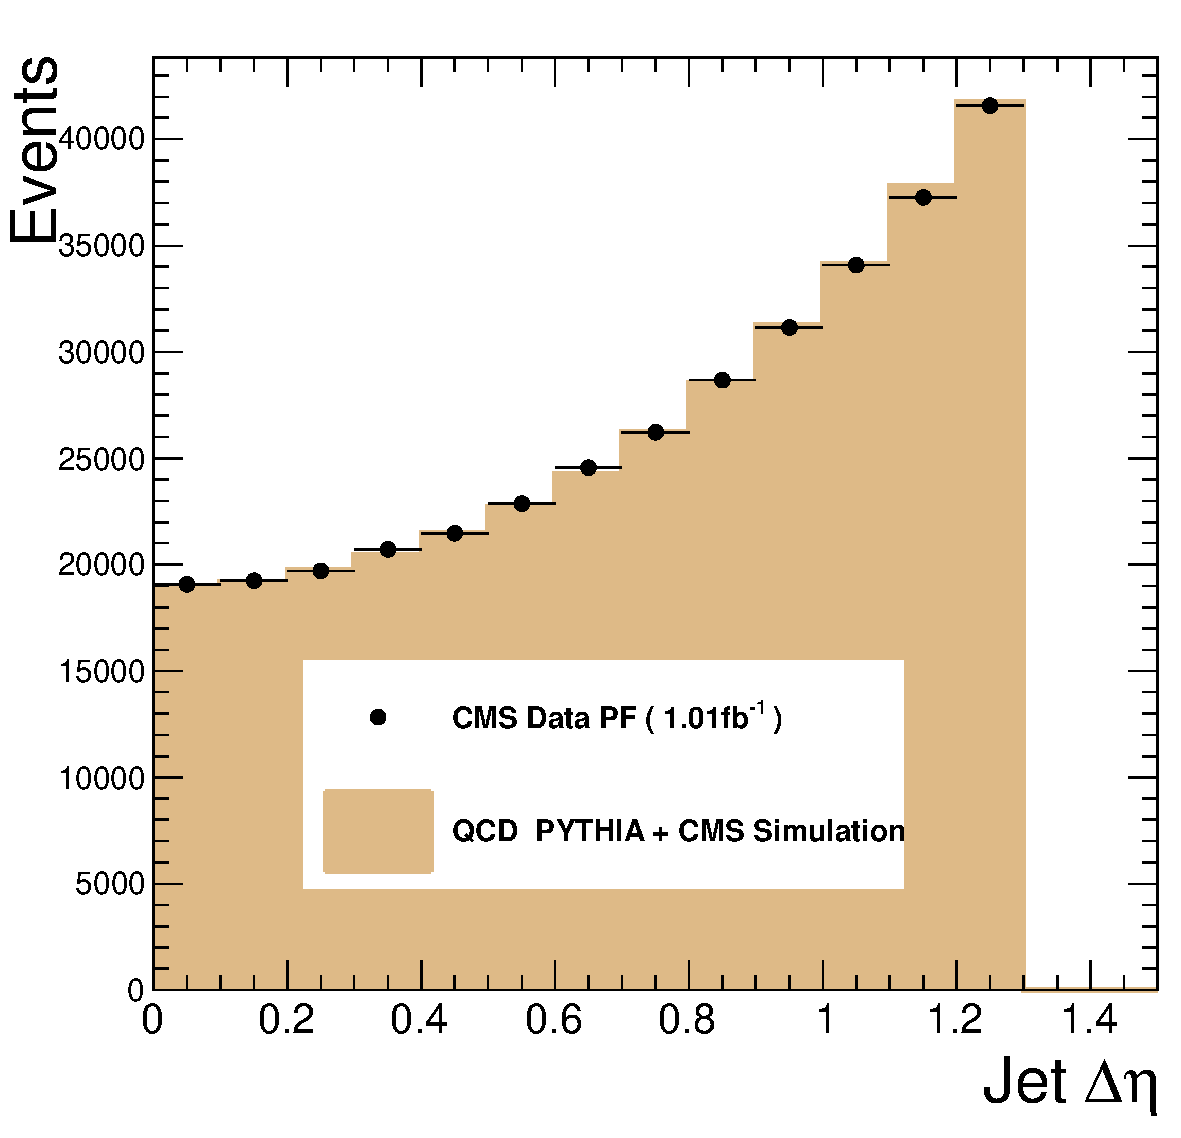
\includegraphics[width=0.45\textwidth]{Figures/c_DEta_pf.pdf}

    \caption{ Jet kinematics distributions for pf jets.  The corrected $P_T$ of
      the two leading jets (upper left) and the same in log scale
      (upper right). The $\eta$ distribution for the two leading jets
      (middle left). The $\phi$ distribution for the two leading
      jets. (middle right) $\phi$ vs. $\eta$ (lower left) for the two
      leading jets. The $\Delta\eta$ distribution (lower right) }
    \label{jet_kinematics_pf}
  \end{center}
\end{figure}

\begin{figure}[!ht]
  \begin{center}
    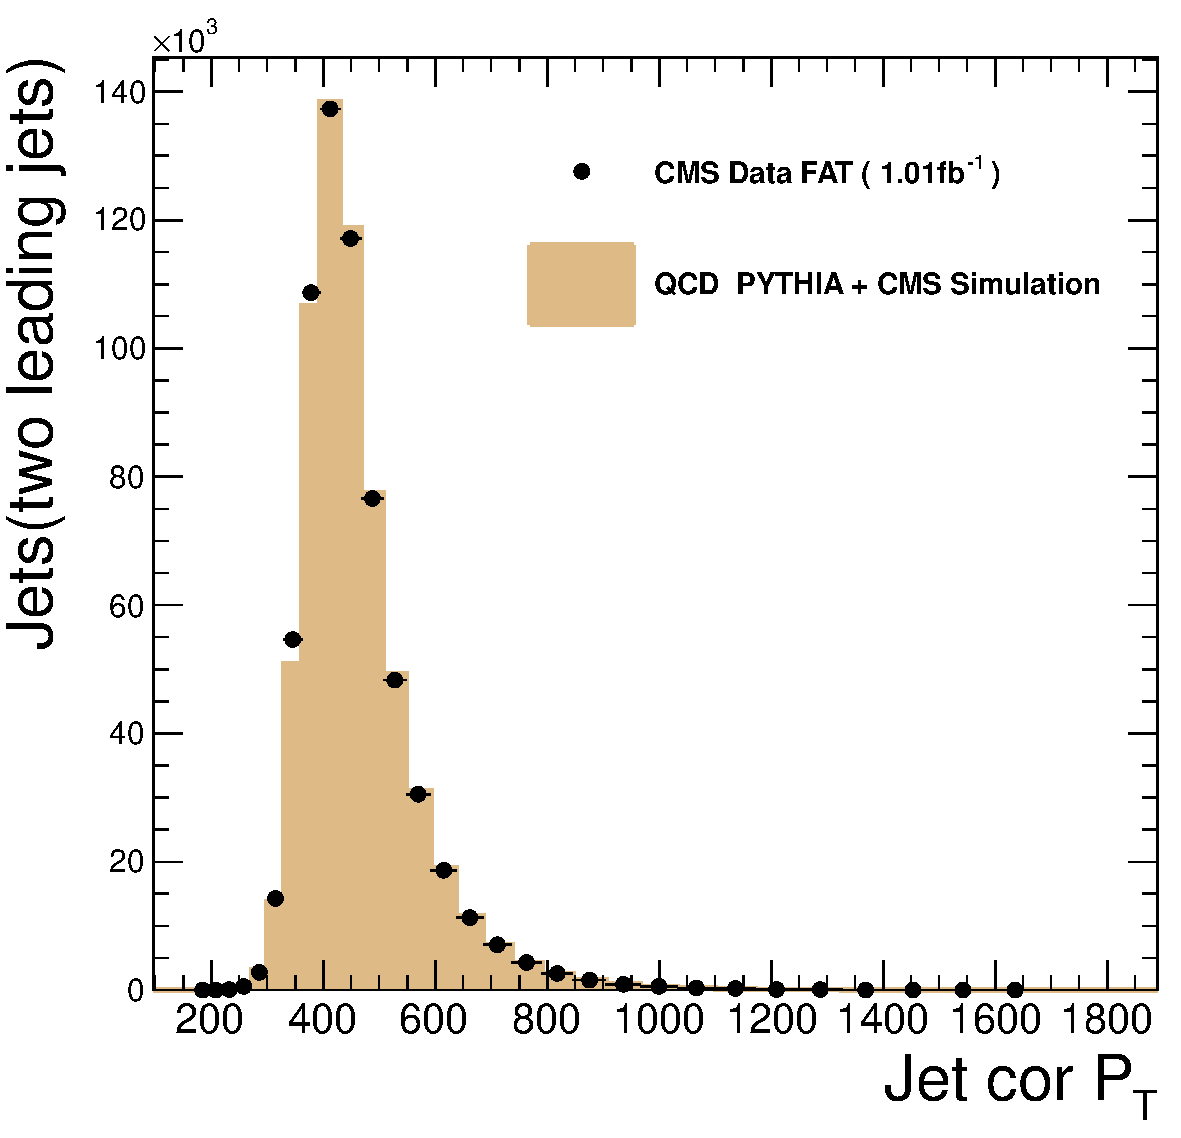
\includegraphics[width=0.45\textwidth]{Figures/c_corPt_fat.pdf}
    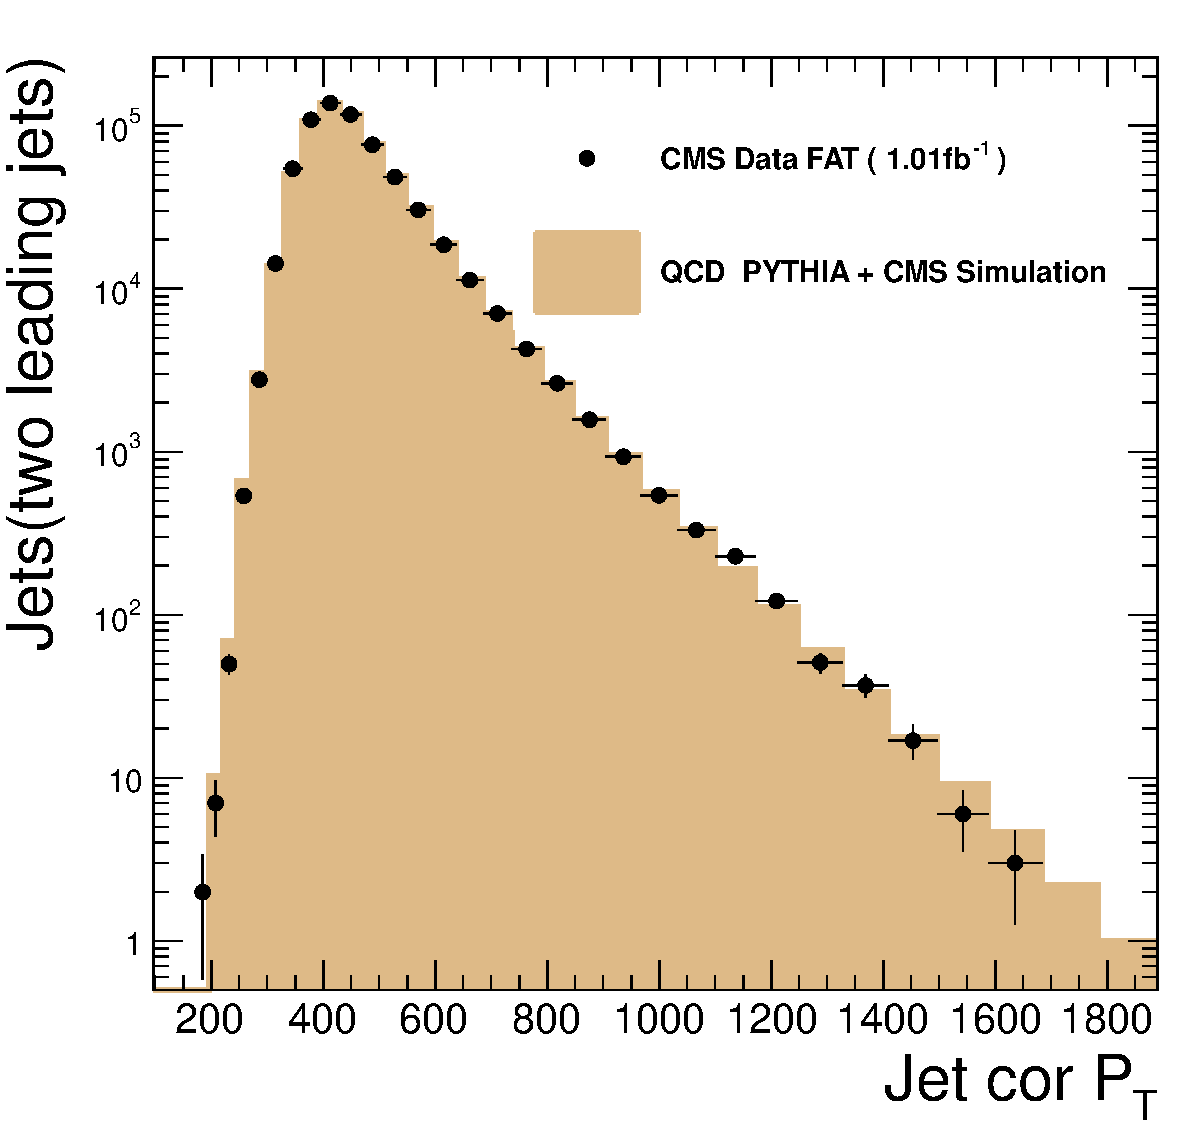
\includegraphics[width=0.45\textwidth]{Figures/c_corPt_fat_log.pdf}
    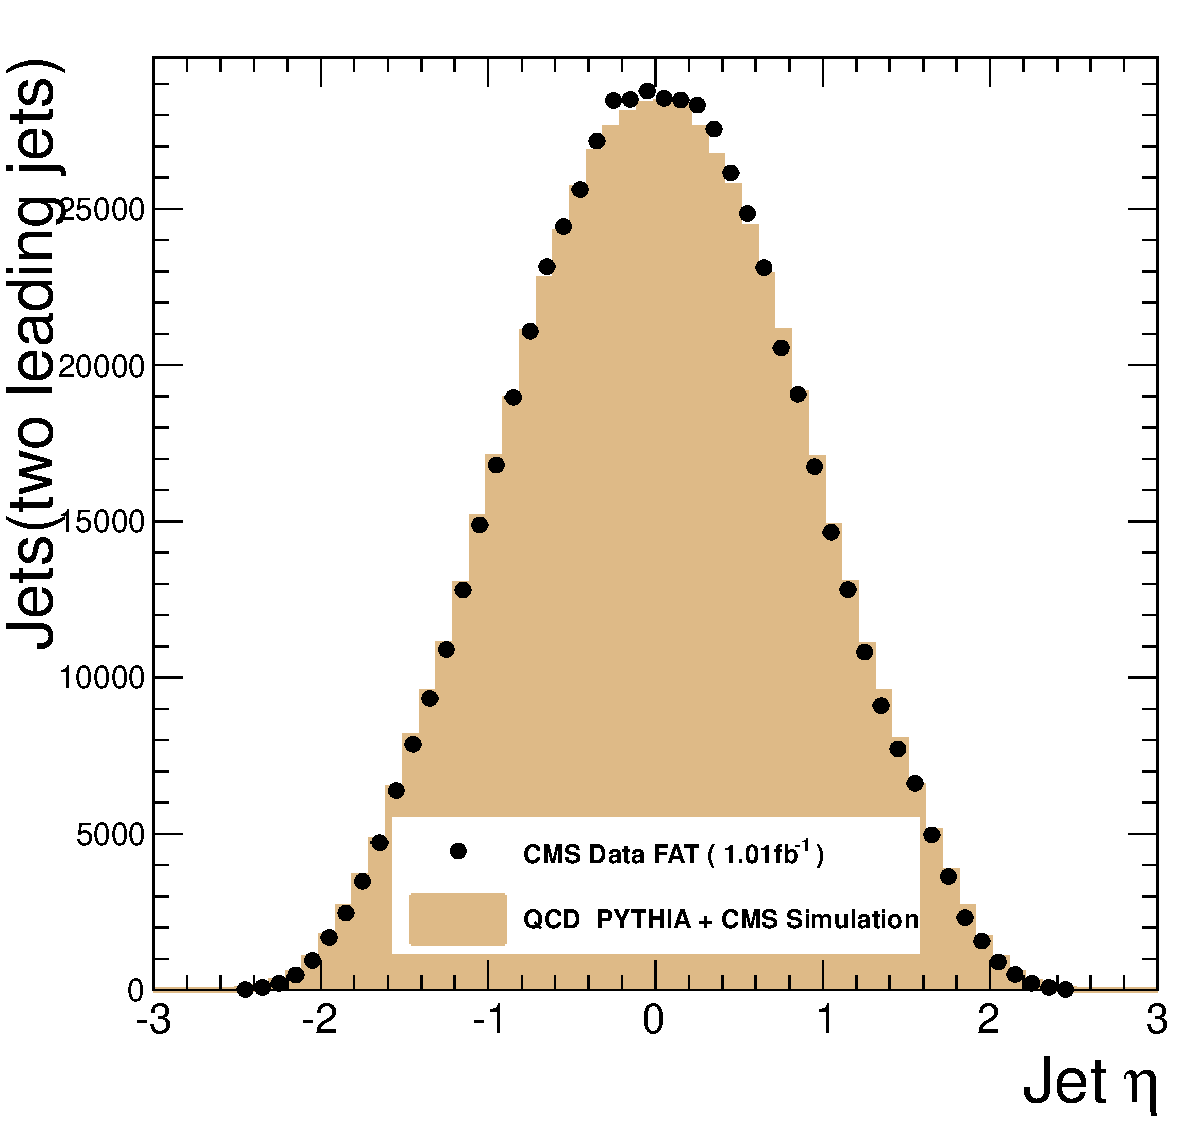
\includegraphics[width=0.45\textwidth]{Figures/c_Eta_fat.pdf}
    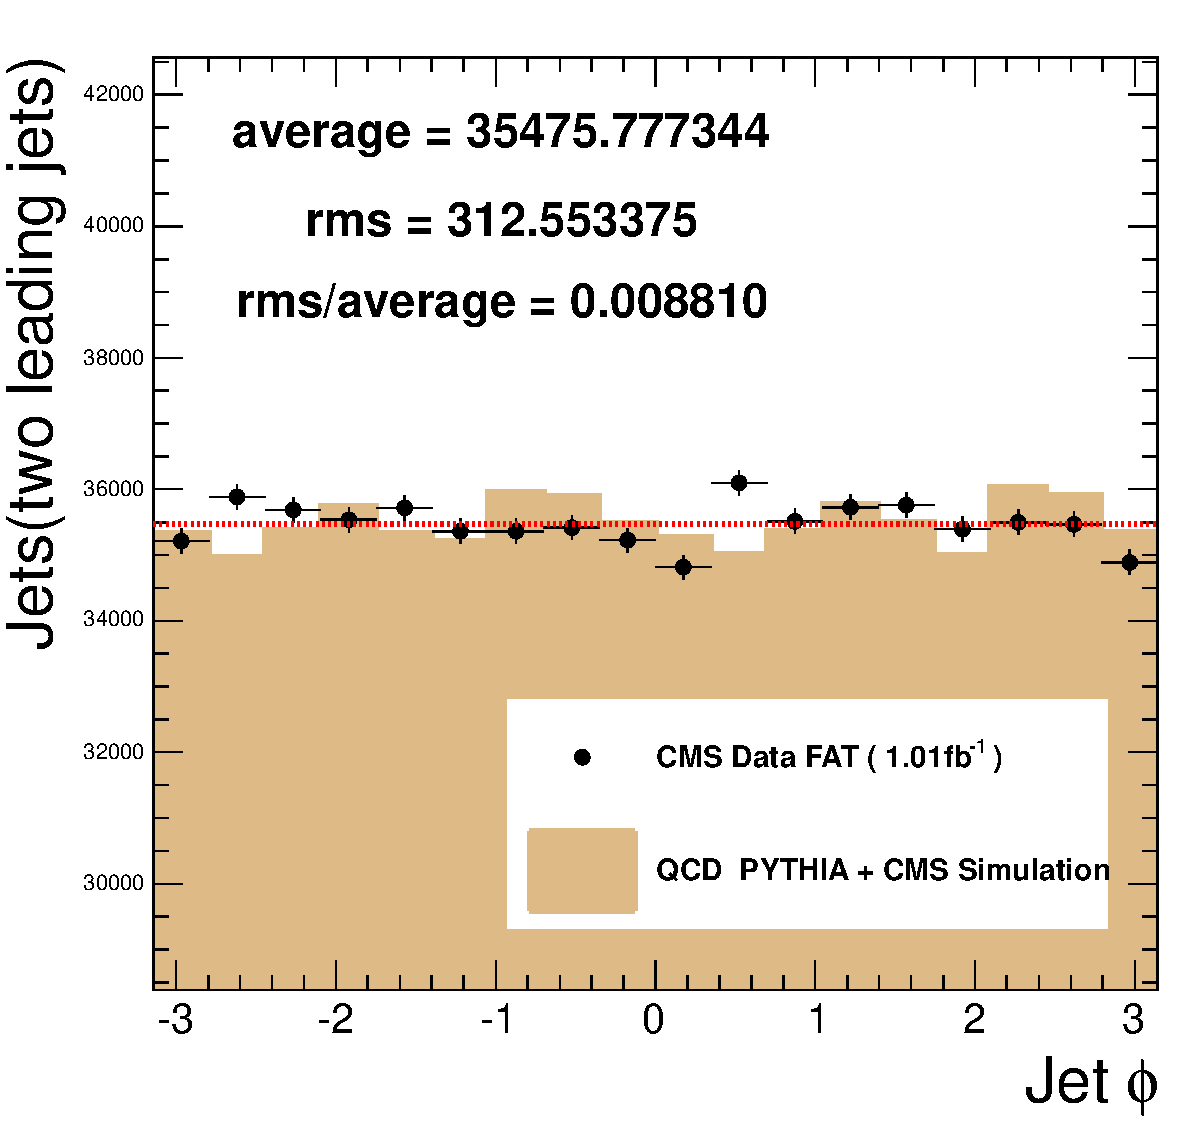
\includegraphics[width=0.45\textwidth]{Figures/c_Phi_fat.pdf}
    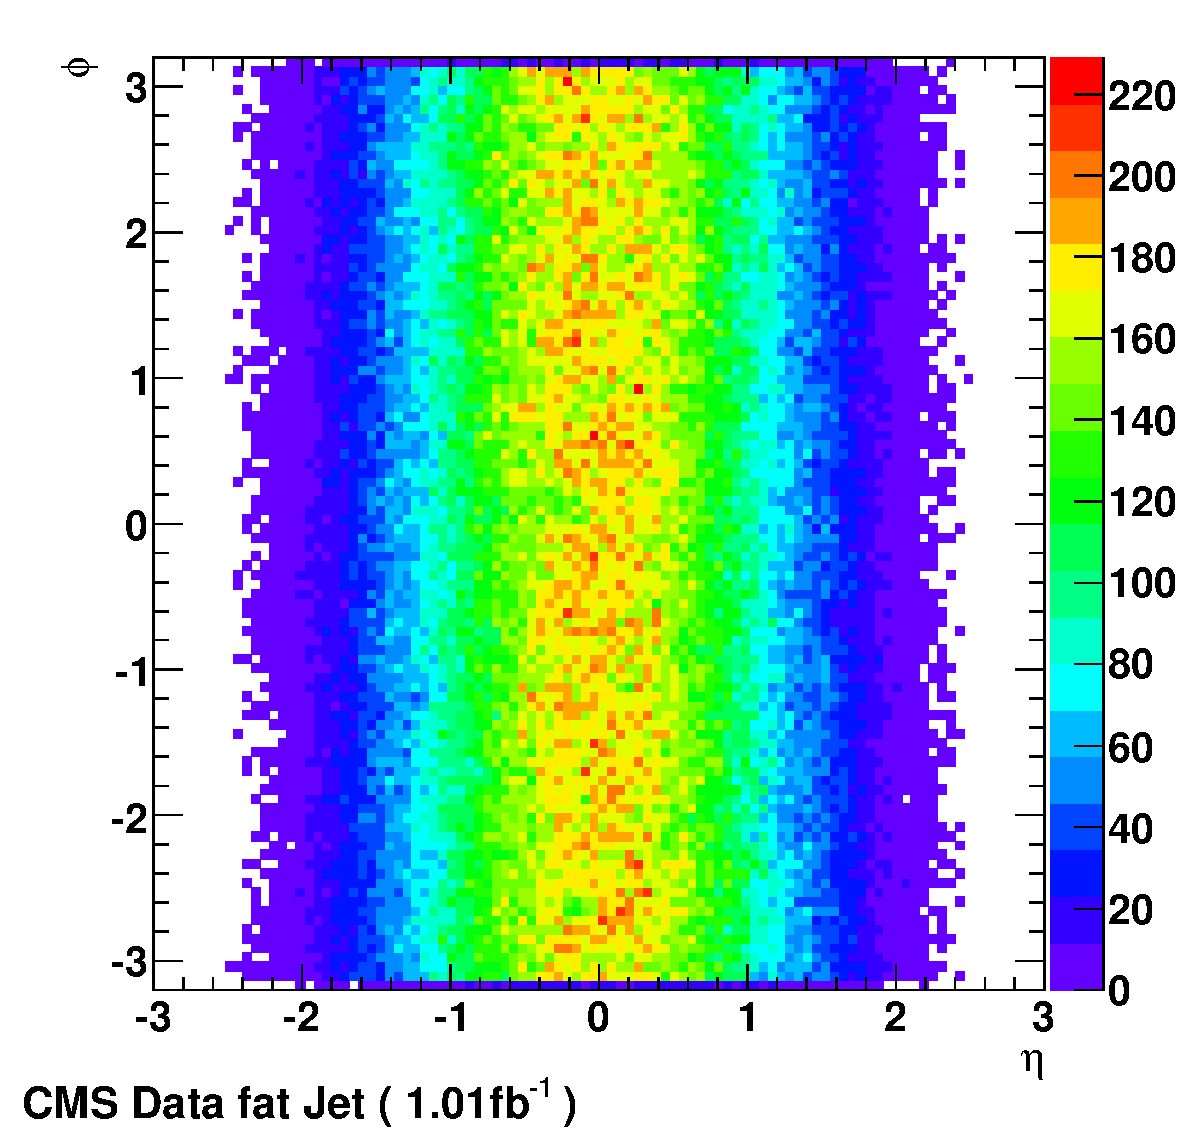
\includegraphics[width=0.45\textwidth]{Figures/c_Eta_Phi_Scatter_fat.pdf}
    \includegraphics[width=0.45\textwidth]{Figures/c_DEta_fat.pdf}

    \caption{ Jet kinematics distributions for wide jets.  The corrected $P_T$ of
      the two leading jets (upper left) and the same in log scale
      (upper right). The $\eta$ distribution for the two leading jets
      (middle left). The $\phi$ distribution for the two leading
      jets. (middle right) $\phi$ vs. $\eta$ (lower left) for the two
      leading jets. The $\Delta\eta$ distribution (lower right) }
    \label{jet_kinematics_wide}
  \end{center}
\end{figure}
%\subsubsection{Dijet Data Stability}
%
%In order to demonstrate the stability of our data as a function of
%run, we show various event and jet related quantities. In
%Fig.~\ref{MassVsRun} we show the number of dijet events surviving the
%full selection, for each run used in the analysis. We also show the
%mean dijet mass vs. run.  In Fig.~\ref{XsecVsRun}, we show the number
%of dijet events divided by the integrated luminosity of each run for
%each run. The observed cross section is well behaved and very stable
%with an RMS of only 2.4\%.
%%, with $\sim 20\%$ fluctuation around
%%the weighted average primarily due to low number of events per run; 
%A minimum luminosity of 1 nb$^{-1}$ in each run is required for the
%plot. The cross section as a function of run is very sensitive to the
%jet energy scale stability which in turn is sensitive to the the
%calibration of the calorimeter. A change of just 0.4\% in the jet
%energy scale between one run and the next would produce a change of
%around 2.4\% in the observed cross section.  In addition, the cross
%section is sensitive to the luminosity evaluation.  The observed
%stability of the cross section is an indication of a stable
%calorimeter energy scale and luminosity evaluation.
%
%In Fig.~\ref{JetPropertiesVsRun} we show the mean value of the basic jet properties (\pt, EMF, number of
%associated tracks), separately for the two leading jets, vs. run. Good stability is observed for all observables.
%
%\begin{figure}[!ht]
%  \begin{center}
%\includegraphics[width=0.9\textwidth]{Figures/MassVsRunNo.pdf} 
%%\includegraphics[width=0.9\textwidth]{Figures/Events.pdf}
%\caption{Mean dijet mass vs run for runs with integrated luminosity greater than $1 nb^{-1}$ .}
%    \label{MassVsRun}
%  \end{center}
%\end{figure}
%
%\begin{figure}[!ht]
%  \begin{center}
%\includegraphics[width=0.90\textwidth]{Figures/XsecVsRunNo_Jet50U.pdf}
%\caption{Number of dijet events passing the full selections, divided by the integrated luminosity of each run, vs. run.
%Only runs with integrated luminosity greater than 1 $nb^{-1}$ passing the analysis selection are shown.}
%    \label{XsecVsRun}
%  \end{center}
%\end{figure}
%
%\begin{figure}[!ht]
%  \begin{center}
%\includegraphics[width=0.49\textwidth]{Figures/PtVsRunNo.pdf}
%\includegraphics[width=0.49\textwidth]{Figures/EmfVsRunNo.pdf}
%\includegraphics[width=0.49\textwidth]{Figures/NtrkVtxVsRunNo.pdf}
%\includegraphics[width=0.49\textwidth]{Figures/NtrkCaloVsRunNo.pdf}
%\caption{Mean value of jet properties for the leading jet (solid circles) and the second jet (open squares) vs. run: 
%\pt (Top-Left), EMF (Top-Right), number of tracks associated with the jets at the vertex (Bottom-Left), number of tracks associated with the jets at the calorimater face (Bottom-Right). Only runs with integrated luminosity greater than $1 nb^{-1}$ are shown.}
%    \label{JetPropertiesVsRun}
%  \end{center}
%\end{figure}
%
\clearpage

\subsubsection{Calo, PF and wide Jet Comparison}

The dijet mass spectrum for Calo Jet Algorithm and PF Jet algorithm are shown
in Fig~\ref{DijetMass_for_Wide_PF_and_Calo}. The overall spectrum shows no big discrepancies
between two algoritms. In the Fig~\ref{DijetMass_compare_Wide_PF_Calo} PF dijet mass is
compared to Calo dijet mass event by event. The ratio distribution plot is also provided
for the events which has Calo dijet mass greater than 2.037TeV. The difference beween PF
and calo dijet mass is less than 0.6\%. Since the JEC uncertainty is bigger, PF and Calo
dijet mass is in reasonable agreement.

\begin{figure}[!ht]
  \begin{center}
   \includegraphics[width=0.45\textwidth]{Figures/c_DijetMass_calo_pf_fat_log.pdf}
    \caption{ The dijet mass spectrum from Wide Jets( black points) is compared to the dijet mass sepectrum from PF Jets (red box) and Calo Jets (blue X) }
    \label{DijetMass_for_Wide_PF_and_Calo}
  \end{center}
\end{figure}


\begin{figure}[!ht]
  \begin{center}
    \includegraphics[width=0.45\textwidth]{Figures/c_DijetMass_PF_wrt_Calo_ak5.pdf}
    \includegraphics[width=0.45\textwidth]{Figures/c_DijetMass_PF_wrt_Calo_2p3TeV_ak5.pdf}
    \includegraphics[width=0.45\textwidth]{Figures/c_DijetMass_PF_wrt_Calo_ak7.pdf}
    \includegraphics[width=0.45\textwidth]{Figures/c_DijetMass_PF_wrt_Calo_2p3TeV_ak7.pdf}
    \caption{ The ratio of corrected dijet mass from PF jets to corrected dijet mass
      from calo jets vs corrected dijet mass from calo jets event by event for ak5. (upper left)
      The ratio distribution for events which has calo dijet mass greater than 2.332 TeV for ak5.
      (upper right)  The ratio of corrected dijet mass from PF jets to corrected dijet mass
      from calo jets vs corrected dijet mass from calo jets event by event for ak7. (bottom left)
      The ratio distribution for events which has calo dijet mass greater than 2.332 TeV for ak7.
      (bottom right) }
    \label{DijetMass_compare_PF_Calo}
  \end{center}
\end{figure}

\subsubsection{Spectrum and QCD}
The measured dijet mass spectrum is shown in Fig~\ref{Spectrum}. The mass spectrum
is defined by 

\begin{equation}
\frac{d\sigma}{dm} = \frac{1}{\int Ldt} \frac{N_{i}}{\Delta m_i}
\label{eqXsec}
\end{equation}
where $m$ is the dijet mass, $N_i$ is the number of events in the
$i$-th dijet mass bin, and $\Delta m_i$ is the width of the $i$-th
dijet mass bin, and the integrated luminosity is $\int Ldt$.  This
data is also tabulated in Appendix~\ref{appData}.  The bin width is
approximately the dijet mass resolution, and gradually increases as a
function of mass.  The data are compared to a QCD prediction from the
PYTHIA MC and the full CMS simulation.  The 
mormalzation of the QCD prediction has been multiplied by a factor of
1.61 to match the data.  Also shown in Fig.~\ref{Spectrum} is the
sensitivity of the QCD + CMS simulation to the systematic uncertainty
in the jet energy scale~\cite{PAS_JME_10-010}. The vertical error bars
on the data are Poisson uncertainties, the horizontal bars are the bin
widths. Bins with zero events are indicated by a Poisson vertical error
bar extending up to 1.8 events.In Fig.~\ref{DataOverPythia_calo} we show the
ratio of the data to the PYTHIA prediction, which demonstrates at a fine
scale the level of agreement between data and PYTHIA. The PYTHIA QCD MC
prediction is in good agreement with the data. 

%This can be seen from summation of the differential plot Fig~\ref{Spectrum} to 
%give the integral plot from the lower bin edge to infinity in Fig~\ref{Integral}. Conservatively,
%we expected 1 event above 1.4 TeV, and we observed 1 event above 1.4 TeV, and it happened to 
%occur at 2.13 TeV.  More aggressively, we expected 0.05 events above 2.1 TeV and we observed 
%1 event, which has a Poisson probability of 5\% which is still only about a 2 $\sigma$ effect.



\begin{figure}[!ht]
  \begin{center}
   \includegraphics[width=\textwidth]{Figures/dijet_mass_Xsec.pdf}
    \caption{ The dijet mass spectrum data (points) is compared to a QCD MC prediction (histogram).
    The QCD prediction has been multiplied by a factor of 1.14 to normalize it to the data.
    The band shows the systematic uncertainty in the spectrum due to jet energy scale
    (conservatively set at 4\%-5\% until we have new JES systematic for 2011).}
    \label{Spectrum}
  \end{center}
\end{figure}

\begin{figure}[!ht]
  \begin{center}
   \includegraphics[width=\textwidth]{Figures/data_over_pythia_fat.pdf}
    \caption{ Ratio of the dijet mass spectrum divided by the QCD Pythia prediction for wide jets. The
    QCD prediction has been multiplied by a factor of 1.09 to normalize it to the data.
    The band showsthe systematic uncertainty in the spectrum due to jet energy
    scale (conservatively set at 4\%-5\% until we have new JES systematic for 2011). }
    \label{DataOverPythia_wide}
  \end{center}
\end{figure}

\begin{figure}[!ht]
  \begin{center}
   \includegraphics[width=\textwidth]{Figures/data_over_pythia_pf.pdf}
    \caption{ Ratio of the dijet mass spectrum divided by the QCD Pythia prediction for pf jets. The
    QCD prediction has been multiplied by a factor of 1.61 to normalize it to the data.
    The band showsthe systematic uncertainty in the spectrum due to jet energy
    scale (conservatively set at 4\%-5\% until we have new JES systematic for 2011). }
    \label{DataOverPythia_pf}
  \end{center}
\end{figure}

\begin{figure}[!ht]
  \begin{center}
   \includegraphics[width=\textwidth]{Figures/data_over_pythia_calo.pdf}
    \caption{ Ratio of the dijet mass spectrum divided by the QCD Pythia prediction for calo jets. The
    QCD prediction has been multiplied by a factor of 1.16 to normalize it to the data.
    The band showsthe systematic uncertainty in the spectrum due to jet energy
    scale (conservatively set at 4\%-5\% until we have new JES systematic for 2011). }
    \label{DataOverPythia_calo}
  \end{center}
\end{figure}

%\begin{figure}[!ht]
%  \begin{center}
%   \includegraphics[width=\textwidth]{Figures/EventIntegral.pdf}
%    \caption{ The integrated event rate above a dijet mass threshold for the data (points) and 
%    the PYTHIA QCD prediction (curve).  The thresholds correspond to the lower edge of the mass bins
%    used in Fig.~\ref{Spectrum} and \ref{DataOverPythia}. The statistical errors on the points are 
%    highly correlated, because each point contains all the other points with higher dijet mass threshold.}
%    \label{Integral}
%  \end{center}
%\end{figure}


%\subsection{Systematic Uncertainty on Jet Energy Scale}
%\label{JESerror}
%The jet energy systematic uncertainty band shown in
%Fig.~\ref{Spectrum} comes from the JetMET official systematics.  It is, the dominant uncertainty
%in the measurement of the dijet mass spectrum, and is also one of the
%largest uncertainties in the new particle search.  
%
%
%As of today we can already see from measurements of photon-plus-jet
%balance~\cite{PAS_JME_10-003, CMS_AN_2010/141} that the jet energy
%scale in the MC may very well be better than the 10\% currently being
%assigned.  The jet response measured with photon + jet balance in the
%data, is in good agreement with the same response measured with the
%MC~\cite{PAS_JME_10-003} and constrain any difference to be well
%within the quoted 10\%. Due to the low statistics and poorly
%understood calibration systematics at this early stage of the
%calibration analysis, JetMET is not quoting an error yet based on this
%data, but JetMET is confident that the data do indicate that 10\% is
%safe.
%
%
%At an even more fundamental level, we already see from measurements of
%single particle response~\cite{PAS_JME_10-008, CMS_AN_2010/179} that
%the barrel calorimeter is responding as expected to input charged
%particles to better than 3\%.  Since a jet is made up of particles the
%uncertainty in the jet response can be constrained by the uncertainty
%in the constituent particle response.  The most uncertain component is
%the charged pion response, as neutral pions are the other dominant
%contributor and they have well understood response in the barrel ECAL.
%The response of the ECAL plus HCAL to isolated charged particles
%measured in the barrel shows excellent agreement between data and
%MC. Further, the MC simulation was tuned on test beam measurements of
%charged pions over a wide range of momentum, and the tuning was quoted
%to be good to within 3\%.  Given these facts, it is highly unlikely
%that the jet energy scale could be off by more than 10\% in the
%barrel.
%
%We have also checked the energy scale of CaloJets against the energy
%scale of particle flow jets in Figure~\ref{PFresp}.  Starting with the
%two leading PF jets in the event with $|\eta|<1.3$, we find the
%matching CaloJets that are closest in $\Delta R$, plot the ratio of
%the corrected CaloJet to corrected PF jet $p_T$, and find the
%mean. The corrected CaloJet $p_T$ is in good agreement with the
%corrected PF jet $p_T$, well within 2\% at all $p_T$, demonstrating
%good agreement between the jet energy scale defined by calorimetry
%alone and the jet energy scale defined by tracking and calorimetry
%combined.
%\begin{figure}[!ht]
%  \begin{center}
%   \includegraphics[width=0.32\textwidth]{Figures/caloRsp_Pt70to84.pdf}
%   \includegraphics[width=0.32\textwidth]{Figures/caloRsp_Pt84to100.pdf}
%   \includegraphics[width=0.32\textwidth]{Figures/caloRsp_Pt100to150.pdf}
%   \includegraphics[width=0.32\textwidth]{Figures/caloRsp_Pt150to200.pdf}
%   \includegraphics[width=0.32\textwidth]{Figures/caloRsp_Pt200to300.pdf}
%   \includegraphics[width=0.32\textwidth]{Figures/caloRsp_Pt300to500.pdf}
%   \includegraphics[width=0.8\textwidth]{Figures/PFvsCalo.pdf}   
%    \caption{Distributions of Corrected CaloJet $p_T$ / Corrected PFJet $p_T$ 
%    for leading jets which have $|\eta|<1.3$ 
%    for six intervals of Corrected PF jet $p_T$ (top six plots) and the mean value of 
%    this relative response as a function of the mean Corrected PF jet $p_T$ 
%    (bottom plot).}
%    \label{PFresp}
%  \end{center}
%\end{figure}
%
%In situ data indicate that the 10\% guideline provided by JetMET on
%the jet energy scale uncertainty is a conservative (safe) estimate.

\subsection{Highest Mass Dijet Events}

Event displays of the three highest mass dijet events are shown in
Appendix~\ref{appEvents}.  They all look like good events, with
collimated calorimeter energy deposits and associated tracks.
Table~\ref{table_highmass2} in the Appendix lists the basic properties
of the calorimeter reconstrution for these events.  The highest dijet
mass observed is at 3.0 TeV as already mentioned.

%In Appendix~\ref{appEvents} in table~\ref{table_highmass3} we list the 
%$p_T$ and dijet mass for these events from particle flow reconstruction
%of the jets (PFjets), which employs tracking in addition to the calorimeter.
%The $p_T$ and dijet mass values are very similar.  Here the PFjets have been
%matched to the corresponding leading CaloJets and are shown in that order
%in table~\ref{table_highmass3}.

%In Fig.~\ref{PF}, we
%show the difference in corrected jet $p_T$ between the leading 
%CaloJets and particle flow jets.
%The mean difference is $\Delta p_T= -0.5$ GeV out of 
%about 300 GeV.  The RMS of the difference between CaloJets and
%PFJets is 15 GeV.  This is in good agreement with the expected RMS from the 
%MC of 18 GeV: this expected RMS takes into account significant correlations 
%between the two reconstruction techniques~\cite{refMikko}. The mean 
%difference of the dijet mass between the two techniques is $2\pm 10$ GeV, 
%and the RMS of the difference in dijet mass is 33 GeV, which makes sense compared
%to $p_T$, but we do not have 
%available an estimate of this RMS from MC that takes into account correlations.
%The good agreement
%between calorimeter and particle flow jet reconstruction techniques for 
%the 10 highest mass dijet events indicates that jet reconstruction with 
%tracking is confiriming our 
%calorimeter based reconstruction technique.


%\begin{figure}[!ht]
%  \begin{center}
%   \includegraphics[width=0.7\textwidth]{Figures/CaloPFCorrelation.pdf}
%    \caption{The difference in corrected jet $p_T$ between the leading CaloJets
%    and the leading matched particle flow jets (histogram) for the 10 highest dijet
%    mass events is compared with an estimate of the expected difference from MC (curve)
%    taking into account correlations. }
%    \label{PF}
%  \end{center}
%\end{figure}
\clearpage

\subsection{Dijet Mass Spectrum and Fit}

\begin{figure}[!ht]
  \begin{center}
   \includegraphics[width=\textwidth]{Figures/DijetMass_withFit_fat.pdf}
    \caption{The dijet mass distribution (points) compared to a smooth background fit wide jets (solid
curve). }
    \label{Fit_wide}
  \end{center}
\end{figure}

\begin{figure}[!ht]
  \begin{center}
   \includegraphics[width=\textwidth]{Figures/DijetMass_withFit_pf.pdf}
    \caption{The dijet mass distribution (points) compared to a smooth background fit PF jets (solid
curve). }
    \label{Fit_pf}
  \end{center}
\end{figure}

\begin{figure}[!ht]
  \begin{center}
   \includegraphics[width=\textwidth]{Figures/DijetMass_withFit_calo.pdf}
    \caption{The dijet mass distribution (points) compared to a smooth background fit for calo jets(solid
curve). }
    \label{Fit_calo}
  \end{center}
\end{figure}

Fig.~\ref{Fit_calo} shows the dijet mass spectrum from Fig.~\ref{Spectrum}
compared to a fit. Here we model the background to a dijet resonance
coming from standard model dijet production using a simple
parameterization. Our first test for whether there is a bump or other
local effect in the data is to simply see if we can get a good fit to
a smooth parameterization.  Fig.~\ref{Fit_calo} also shows the
parameterization fitted to the data. We get a $\chi^2$ of 25.67 for 23
degrees of freedom for the fit.  The parameterization chosen
is~\cite{Aaltonen:2008dn,ATLAS_Search}


\begin{equation}
\frac{{\rm d}\sigma}{{\rm d}m} = 
\frac{P_{0} (1 - m/\sqrt{s})^{P_{1}}}{(m/\sqrt{s})^{P_{2} + P_{3} ln
(m/\sqrt{s})}}
\label{eqParam}
\end{equation}

Fig~\ref{FracDiff_calo} shows the fractional differences between data and
the fit function, (data-fit)/fit, which show no significant evidence
of a peaks above the background fit. 
%The most significant upward
%fluctuation observed is studied in section~\ref{significance}.  
In the
fractional difference plot the error bars are in units of the fit in
the bin.  Fig.~\ref{FracDiff_calo} show the pulls, defined as \textit
{(Data-Fit)/Error}, which are consistent with statistical fluctuations
and are scattered around zero. In the pulls plot the error bars are
always exactly 1, because they are in units of the error in the bin.

\begin{figure}[!ht]
  \begin{center}
    \includegraphics[width=0.7\textwidth]{Figures/Fractional_Diff_fat.pdf}
    \includegraphics[width=0.7\textwidth]{Figures/Pulls_fat.pdf}
    \caption{ \textit{Top}) The fractional difference between the
dijet mass distribution (points) and a smooth background fit as a
function of dijet mass for wide jets. \textit{Bottom}) The pulls distribution
(Data-Fit)/Error as a function of dijet mass.}
    \label{FracDiff_wide}
  \end{center}
\end{figure}

\begin{figure}[!ht]
  \begin{center}
    \includegraphics[width=0.7\textwidth]{Figures/Fractional_Diff_pf.pdf}
    \includegraphics[width=0.7\textwidth]{Figures/Pulls_pf.pdf}
    \caption{ \textit{Top}) The fractional difference between the
dijet mass distribution (points) and a smooth background fit as a
function of dijet mass for pf jets. \textit{Bottom}) The pulls distribution
(Data-Fit)/Error as a function of dijet mass.}
    \label{FracDiff_pf}
  \end{center}
\end{figure}

\begin{figure}[!ht]
  \begin{center}
    \includegraphics[width=0.7\textwidth]{Figures/Fractional_Diff_calo.pdf}
    \includegraphics[width=0.7\textwidth]{Figures/Pulls_calo.pdf}
    \caption{ \textit{Top}) The fractional difference between the
dijet mass distribution (points) and a smooth background fit as a
function of dijet mass for calo jets. \textit{Bottom}) The pulls distribution
(Data-Fit)/Error as a function of dijet mass.}
    \label{FracDiff_calo}
  \end{center}
\end{figure}

\clearpage
%%%%%%%%%%%%%%%
\subsubsection{Fit to Dijet Mass Spectrum with Various Parameterizations}
\label{sectionParam}

 
In Fig.~\ref{dijetmassFitParams_calo} we show the dijet mass distribution,
$d\sigma/dm$, fit with three different parameterizations: our default
4 parameter fit and two alternate fits.
%%%%%%%%%%%%%%%%%%%%

\begin{figure}[!ht]
  \begin{center}
        \includegraphics[width=\textwidth]
                        {Figures/DijetMass_withFit_All_fat.pdf}
    \caption{ 
The dijet mass data (points) is compared to fits for wide jets(curves)
using our default fit function and three alternate fit functions.}
    \label{dijetmassFitParams_wide}
  \end{center}
\end{figure}

\begin{figure}[!ht]
  \begin{center}
        \includegraphics[width=\textwidth]
                        {Figures/DijetMass_withFit_All_pf.pdf}
    \caption{ 
The dijet mass data (points) is compared to fits for pf jets(curves)
using our default fit function and three alternate fit functions.}
    \label{dijetmassFitParams_pf}
  \end{center}
\end{figure}


\begin{figure}[!ht]
  \begin{center}
        \includegraphics[width=\textwidth]
                        {Figures/DijetMass_withFit_All_calo.pdf}
    \caption{ 
The dijet mass data (points) is compared to fits for calo jets(curves)
using our default fit function and three alternate fit functions.}
    \label{dijetmassFitParams_calo}
  \end{center}
\end{figure}


\clearpage
The parameterizations are listed in equation~\ref{eqVariousParams}.

%%%%
\begin{eqnarray}
{\frac{d\sigma}{dm}} 
 &=& {\frac{P_{0} \cdot (1 - m/\sqrt{s})^{p_{1}}}{(m/\sqrt{s})^{p_{2} + p_{3} ln(m/\sqrt{s})}}} \, \, \, \mbox{(Default Fitwith 4 parameters)}. \cr
 & & \cr
 &=& {\frac{P_{0} \cdot {\Big(1-m/\sqrt{s}+P_3\cdot(m/\sqrt{s})^2\Big)^{P_1}}}{m^{P_{2}}}} \, \, \,\mbox{ (Alternate Fit A with 4 parameters)}. \cr
 & & \cr
 &=& {\frac{P_{0} \cdot {(1-m/\sqrt{s}\,)^{P_1}} }{m^{P_{2}}}}, \, \, \, \mbox{(Alternate Fit B with 3 parameters)} \cr
\label{eqVariousParams}
\end{eqnarray}
%%%%


The default four-parameter function was used by CMS in the published
paper based on 3 pb$^{-1}$, CDF in run
II~\cite{Aaltonen:2008dn}, and is used by ATLAS~\cite{ATLAS_Search}. It
gives a good fit with $\chi^2/DF=25.67/23$.  We have also explored two
alternate parameterizations.  All parameterizations have a power law
in them, because without a power law we cannot get a good fit with
only 3 or 4 parameters.

Alternated fit B is a three-parameter fit that was used by CDF in run
IA~\cite{Abe:1995jz} and has the simplest QCD motivation, although
all the parameterizations are motivated in a similar fashion.  It was
used in much earlier versions of this CMS analysis with significantly
less luminosity.  It has a term in the numerator motivated by the
parton distribution fall off with fractional momentum, the same term
as in the numerator of our default fit.  It includes a power law fall
off with mass in the denominator, motivated by the QCD matrix
element. It also fits the data well.

Alternate fit A is a four-parameter function that was used by CDF in
run IB~\cite{Abe:1997hm}.
It similar to alternate fit B, except it has an additional term in the
numerator to give flexibility beyond the 3-parameter fit.
It also fits the data well.
Since this parameterization has the same number of
parameters as our default fit, we use it to evaluate systematics on
the background functional form. 

Figure~\ref{dijetmassFits_calo} shows the fractional 
differences between data and the fit function, (data-fit)/fit, 
and the pulls, (data-fit)/error, for all three fits.

%%
\begin{figure}[!ht]
  \begin{center}
        \includegraphics[width=0.7\textwidth]{Figures/Fractional_Diff_All_fat.pdf}
        \includegraphics[width=0.7\textwidth]{Figures/Pulls_All_fat.pdf}
    \caption{ Top) Fractional difference (points) between the dijet mass distribution 
data and four fits as a function of dijet mass for wide jets.
Bottom) Pulls for the data (points) compared to four fits as a function of dijet mass.}
    \label{dijetmassFits_wide}
  \end{center}
\end{figure}

\begin{figure}[!ht]
  \begin{center}
        \includegraphics[width=0.7\textwidth]{Figures/Fractional_Diff_All_pf.pdf}
        \includegraphics[width=0.7\textwidth]{Figures/Pulls_All_pf.pdf}
    \caption{ Top) Fractional difference (points) between the dijet mass distribution 
data and four fits as a function of dijet mass for PF jets.
Bottom) Pulls for the data (points) compared to four fits as a function of dijet mass.}
    \label{dijetmassFits_pf}
  \end{center}
\end{figure}

\begin{figure}[!ht]
  \begin{center}
        \includegraphics[width=0.7\textwidth]{Figures/Fractional_Diff_All_calo.pdf}
        \includegraphics[width=0.7\textwidth]{Figures/Pulls_All_calo.pdf}
    \caption{ Top) Fractional difference (points) between the dijet mass distribution 
data and four fits as a function of dijet mass for calo jets.
Bottom) Pulls for the data (points) compared to four fits as a function of dijet mass.}
    \label{dijetmassFits_calo}
  \end{center}
\end{figure}

%\begin{figure}[!ht]
%  \begin{center}
%        \includegraphics[width=0.8\textwidth]
%                        {Figures/dijet_mass_Fit_FracDiff_23params.pdf}
%    \caption{
%    Fractional difference between the dijet mass distribution 
%data points and the 2-parameter fit (left) and the 3 and 4 parameter fits (right).}
%    \label{dijetmassFractionalDiffFit23params}
%  \end{center}
%\end{figure}
%%%%%%%%%%%%%%%%%%%%

\clearpage
